
\chapter{Opponent Modelling}
\label{c:opponentmodelling}

After having outlined the algorithms necessary to make a decision based on the game context, there still stays an unresolved issue; how to determine the probability distribution of an opponents possible action and the hands he might hold.  Both in computer as in human poker, a good judgement of the opponent is required. A player must be able to predict the opponents actions, as well as figuring out what cards he might hold. Essentially, the target is to estimate the missing information in this game of imperfect information. 

To achieve this, a model of the opponent has to be created. This model could be very generic; based on historic averages or game-theoretic optima, both very static models.  But playing good poker also includes adapting to a specific player, learning his strengths and weaknesses and exploiting them. To achieve this, the opponent model can't be merely static, but has to adapt to the current opponent, or even the current style the current opponent is playing. ideally, a good opponent model would never reaches a stable conclusion, but continue to adapt to the current opponent as well as his style at every moment.

Little surprising, as \cite{Pena1999} has shown, specific (based on observations of the the current opponent) opponent modeling outperforms generic opponent modeling.

To predict actions and cards, there exist a multitude of methods. From basically non-modeling but calculating the game theoretic best actions (used in all basic game theoretic methods of \cite{Gilpin2006} \cite{Johanson2007} or \cite{Miltersen2007}, used in \cite{Billings2006b} and \cite{Schauenberg2006} as a default prior of the model), to neural networks and decision trees.


\section{Optimal versus Maximal Play}
\label{sec:optimalvsmaximal}

One important consequence of imperfect information is that a complete strategy for a game like poker must include a certain degree of deception. It can by very rewarding to bluff (betting or raising with a weak hand) or slow play (playing a strong hand as though it were weak), not only because it might lead to winning a hand with weak cards, but also to add some noise to the revealed information. As \cite{Billings2006} explains, the requirement for such deceptions was one of the earliest results in game theory \cite{Neumann1944}. Essentially, it's always best to reveal as little information as possible, to act as unpredictably as possible.

In Poker, the target of deception tactics is it to disguise the strength of a hand (information hiding), and to create uncertainty for the opponent. As \cite{Billings2006} explaines, the relative balance of these deceptive plays (and of responses to the opponent's actions) is of critical importance. Any inappropriate imbalances necessarily imply the existence of statistical biases, patterns, or other weaknesses that are vulnerable to exploitation. Since there may be many ways of obtaining the desired balance of plays in poker, the players have some discretion in how they actually achieve that balance. In essence, it might not matter if, in a specific situation, a player bluffs or doesn't, as long as a certain bluff frequency in this and similar situation is maintained. As a often stressed result, there is in general no single best move in a given poker situation  \cite{Sklansky1999} \cite{Chen2006} (but in theory, there might be a best distribution of moves). This is a huge difference to perfect information games, where a single move can be determined to lead to the game-theoretic maximum.

As \cite{Billings2006} notes, correct play in an imperfect information game requires probabilistic mixed strategies, where different moves are chosen some fraction of the time in identical circumstances. In a perfect information game though, a deterministic pure strategy (always playing one particular move in a given situation) is sufficient to obtain
the game-theoretic value although the player may choose randomly from a set of equally valued moves).

It's important to understand the difference between optimal and maximal play. Optimal play is a result of a equilibrium strategy. In games like poker, where weaknesses of an opponent be systematically exploited, an equilibrium strategy is only maximal against an equilibrium playing opponent (an opponent without any exploitability).

In a Nash equilibrium strategy, no player has an incentive to deviate from the strategy, because the alternatives only lead to equal or worse results. This simply maximizes the minimum outcome. In essence, this is a defensive strategy which assumes the opponent plays perfect, and the player only tries to not loose. In practice, outside of very simple games like tic-tac-toe, no such player exists, especially not in poker. Only a very small fraction of games have been game theoretically solved. And it's questionable if some of them ever will, since the search space for games like chess, go or larger poker games is just too enormous.

Not only might a Nash equilibrium player not play an optimal strategy, in certain situations he might not even defeat a non-optimal opponent.  For example, in the game of rock-paper-scissors, the equilibrium strategy is to select an action uniformly at random among the three choices. Using that strategy means that no one can defeat you in the long term, but it also means that you will not win, since the equilibrium player has an expected value of zero against any other strategy.

Unlike rock-paper-scissors, poker is a game in which some strategies are dominated, and could potentially lose to an equilibrium player. Nevertheless, even a relatively weak and simplistic strategy might break even against a Nash equilibrium opponent, or not lose by very much over the long term. 

In contrast, a maximal player can make deviate from an "optimal" strategy when it believes that such a move has a higher expected value.  \cite{Johanson2007} employs such a strategy in his approach for a best response strategy, based on different $\epsilon$-equilibria strategies.

Considering the case of rock-paper-scissors where a opponent has played "rock" 100 times in a row, a Nash equilibrium program is completely oblivious to the other player's tendencies, and does not attempt to punish predictable play in any way. A maximal player, on the other hand, will attempt to exploit perceived patterns or biases. This always incurs some risk (the opponent might have been setting a trap with the intention of deviating on the 101st game). A maximal player would normally accept this small risk, playing "paper" with a belief of positive expectation \cite{Billings2006}. Similarly, a poker program can profitably deviate from an equilibrium strategy by observing the opponent's play and biasing its decision-making process to exploit the perceived weaknesses.

If a poker algorithm were based on a true Nash equilibrium solution, then no human or computer player could expect to defeat it at all in the long run. However, all current poker programs are only an approximation of an equilibrium strategy (\cite{Johanson2007}, \cite{Gilpin2007} etc.), and it will not be feasible to compute a true Nash equilibrium solution for Texas Hold'em in the foreseeable future. There is also an important practical limitation to this approach.

Additionally, simple equilibrium approximations are unintentionally exploitable. Since they apply a fixed strategy, a strong human player can systematically explore various options, probing for weaknesses without fear of being punished for using a highly predictable style. Moreover, the key to defeating all human poker players is to exploit their highly
non-optimal play. 
When humans play games, especially at a more professional level, they analyze previous games played by their opponent to become familiar with the strategies used by the opponent, its strengths and weaknesses. Even when playing against
an unknown player, they will create, during the game, a model of the opponent, based on some features of the opponents behavior. To compete at such a level of skill, a computer poker program would also be required to be able to adapt to an opponents play and adapt to dynamically changing conditions. \cite{Billings2006}

\section{Challenges in Opponent Modelling}

As we have seen in the last chapter, for poker, we need our opponent model to predict two things in the game tree. First, what action a player might take, given a certain situation. Second, how strong his cards might be, given a certain situation. As we will see, this task faces challenges, shared with many other machine learning or data mining problems. \cite[p.36-37]{Davidson2002} summarizes them as follows:

\begin{itemize}
	\item \textbf{Uncertainty:} Thanks to the numerous unknown cards in a game, poker games always include a great deal of noise. Each hand of poker can be completely different to the previous one, simply because of the variance of cards dealt. Both to the hands as well as to the board. Because of this, a very large number of hands must be played bevor even very common situations are encountered several times.
	\item \textbf{Missing Information:} Only the player and his opponent play to the end of a hand, cards are actually shown. In heads-up only a very small percentage of hands are revealed. Because of this, the opponent model can only be verified on the very few hands the player as well as the opponent take to the showdown. Additionally, these hands are obviously heavily biased (players always try to avoid taking bad hands to a showdown - either by folding or by getting the opponent to fold).
	\item \textbf{Unknown Dimensions:} It's never completely known what variables, and how many of them affect how a player plays a hand. Some factors might be much more important than others, and some are not of concern for every player. One might put importance into their position in the betting round, while others only adapt lightly to their position. To find the appropriate correlations is important, but very difficult. 
	\item \textbf{Intuition:} Thanks to intuition and past experience, good human Players are able to form an elaborate model of the opponent based on only a small number of observations. If experienced, they can also challenge their model to test a theory about an opponent. In contract, most machine learning methods typically need a large number of observations. These methods are not only slow, but also passive.
	\item \textbf{Multiple Levels:} If we model an opponent based on how he plays against another player, we can't regress his behavior playing against us, at least not if he is also modeling his opponents. So we need find a "pure" model (the opponents behavior minus his adaptations to a certain player) as well as how he models opponents. (or how he models how we model, etc...)
	\item \textbf{Moving Targets:} To play good poker also means to constantly change once behaviour, simply to add noise to the opponents observations. This and the fact that the opponent might change his model about us, presents the problem that the opponent model has to be changed constantly, and that once we achieve a solid model, this model is already outdated.
\end{itemize}

To summarize, opponent modeling contains the typical characteristics of most machine learning problems;noise, uncertainty, unknown relations, and the need to quickly generalize from a small set of examples - often with wrong or misleading data.  


\section{Opponent Modelling Techniques}
\label{opponent-modelling-techniques}
As we don't know the hands of the opponent, we can't perfectly predict what an opponent play, but a distribution of actions. Considering machine learning, an opponent model is a predictor of the opponent. In the data mining approach outlined later, it's simply a matter of classifying a certain decision point or game situation into possible opponent action classes. \cite[p.37]{Davidson2002} outlines the basic methods of opponent modeling, which are shortly outlined hereby. Most of these techniques can also be used in the later introduced \textit{Weka Data Mining Framework} and can be applied to the algorithm described in chapter ~\ref{c:imperfectinformation}.

\subsection{Expert Systems}
Expert Systems are implementing a generic opponent model, crafted after human knowhow and implemented as a set of rules. One way would be to predict an opponent action based on our own betting strategy, or advice out of a poker strategy book. Expert Systems normally aren't very effective, since they scale very bad for complex problems, but they are a good start for a opponent model, per example before any knowhow about a specific opponent could be collected.

\subsection{Statistics}
\label{s:statistics}
Another rather obvious method of predicting an opponent is observing his past actions, assuming he would act the same or similar in the future. If he raised 10\% of our bets on the flop, after a lot of action already happened pre-flop, one might infer that the next time such a situation occurs, the possibility of our opponent to raise is 10\%.


\cite{Davidson2002}'s opponent modeling effort was based on a collection of simple statistic information. For example, a basic system distinguished only twelve different contexts a player might encounter. These twelve contexts differ only in the betting round (pre-flop, flop, turn, or river), and the betting level (zero, one, or two or more bets)

The resulting history table is essentially a set of conditional action probabilities such as \linebreak $P(OneBetToCall,stage=river)$ - describing the probability of a raise, given there was one bet this hand so far, and the decision will be made on the river. 

However, this is a very limited definition of distinct contexts, since it does not account for many relevant properties, such as the number of active opponents, the relative betting position, or the texture of the board cards (eg. whether or not many draws are possible). 

Establishing a suitable set of conditions for defining the various situations is not an easy task. There are
important trade-offs that determine how quickly the algorithm can learn and apply
its empirically discovered knowledge. If a context is defined too broadly, it will fail to
capture relevant information from very different circumstances. If it is too narrow,
it will take too long to experience enough examples for each scenario, and spotting
general trends becomes increasingly difficult. Equally important to deciding how
many equivalence classes to use is knowing what kinds of contextual information
are most relevant in practice.


One such model, is the histogram-based approach by \cite{Schauenberg2006} and \cite{Billings2006b}.  Essential for using such statistical modeling, it a good abstraction of the game context. 

In poker, two situations rarely happen twice, even after millions of hands, so the need for generalization arises. For their Miximax-based agents,  \cite{Schauenberg2006}  and \cite{Billings2006b} used a collection of histograms with different levels of generalization. To learn faster and base their inferences on more observations, \cite{Billings2006b} use various different context trees with different granulation, and combine multiple contexts with high mutual correlation.  This allows them to generalize the observations made, and apply that knowledge to other related situations.

The context tree they used is an explicit representation of the imperfect information game tree, having the same skeletal structure with respect to decision nodes. Chance nodes in the tree are represented implicitly (all possible chance outcomes are accounted for during the EV calculation).

A leaf node of the context tree corresponds to all of the leaves of the game tree with the same betting sequence (regardless of the preceding chance nodes).

Associated with this is an efficient data structure for maintaining the empirically observed action frequencies and showdown histograms for the opponent. For this they use a trie, based on the natural prefix structure of related betting sequences.
 
The finest level in the abstraction is the context tree itself, where every possible betting sequence is distinct, and a different histogram is used for each. This basically is a reproduction of all possible game situations.  The
opponent action frequencies are determined from the number of times each action was chosen at each decision node (they also used a decay factor, to strengthen recent observations). Unfortunately, having little data in each class will result in unreliable inferences.

With testing, they concluded, that the most coarse-grained abstraction would solely hold the sum of the total number of raises by both player (no longer distinguishing which player initiated the action) - in total only nine distinct classes. Despite the crudeness of this abstraction, the favorable effects of grouping the data is often more important than the lower expected correlations between those lines of play. Another similar type of coarse-grained abstraction considers only the final size of the pot, adjusting the resolution (i.e. the range of pot sizes) to provide whatever number of abstraction classes is desired.

A less coarse-grained abstraction groups all betting sequences where the opponent made an equal number of bets and raises throughout the hand, ignoring what stage of the hand they were made. A finer-grained version of the same idea maintains an ordered pair for the number of bets and raises by each player.

 One problem with a statistical approach to opponent modeling is the zero frequency problem, when there has not yet been any observations for a given context - and more generally, how to initialize the context tree with good default data. \cite{Billings2006b} depend on results from Nash equilibrium strategies, to devise default data based on the assumption of optimal play.

\cite{Schauenberg2006} and \cite{Billings2006b} use various different abstractions of situations and weights them differently before predicting a situation. One extreme would be the exactly same situation, another every other situation with the same amount of player actions in the hand so far. Based on this  \cite{Billings2006b}  specified 8 different abstractions which he averaged to calculate the action distribution of possible actions. \cite{Schauenberg2006}, \cite{Billings2006b} and \cite{Davidson2002} don't take the public board cards into consideration when looking for similar situations.

Establishing a suitable model on how broad or narrow a situation should be specified is no easy task. There's an obvious trade-off of being either to narrow, so there are not enough samples to base assumptions from, or being to broad, so estimations will be vulnerable to over-fitting. 

Furthermore, each player acts differently. One might be very affine to flush draws and play them very aggressively, another might put a lot of weight in his current chip stack before deciding how to act. To model this, a meta-model would have to be built of the player, to specify which parameters are weighted how much in the modeling process. 
Using data mining algorithms and a very large set of parameters might be a good approach for this problem, since figuring out the weight of the different parameters is a common problem in other classifying problem.

As the abstraction system of  \cite{Billings2006b} is hierarchical, there also has to be spent some consideration into the weight of the different tiers of abstraction. This is based on the number of actual observations covered at each level, striving for an effective balance, which will vary depending on the opponent.

Their method of combining different abstraction classes is based on an exponential mixing parameter (e.g. $m = 0.95$). With the lowest-level context tree (no abstraction) be called $A_0$, a fine-grained abstraction be called $A_1$, a cruder collection of those classes be called $A_2$, and the broadest classification (only pot-size or only count of bets) level be called $A_3$. 

Suppose the showdown situation in question has five data points (earlier observations) that match the context exactly, in $A_0$. This data is given a weight of $1-m^5 = 0.23$ of the total. If the next level of abstraction, $A_1$, has 20 data points (including those from $A_0$), it is assigned $1-m^20 = 0.64$ of the
remaining weight, or about $50\%$ of the total. The next abstraction level might
cover 75 data points, and be given $1-m^75 = 0.98$ of the remainder, or
$26\%$ of the total. The small remaining weight is given to the crudest level of
abstraction. Thus all levels contribute to the overall profile, depending on how
relevant each is to the current situation.

After each hand is finished, the observations made must be applied to the histograms in the context tree.  The action decisions made by the opponent are used to update the betting frequencies corresponding to the sequence of actions during the hand, while the shown cards (respectively, the hank rank of the cards) are used to update a leaf node histogram.

The context basically represents the imperfect information tree which is searched when looking for the correct action. It has the same decision nodes, but is lacking the explicit representation of the chance nodes. A leaf node of the context tree corresponds to all of the leaves of the game tree with the same betting sequence (regardless of the preceding chance nodes).

Since in poker a situation rarely occurs twice, many thousands of games may have to be observed before a reliable histogram of an opponents actions might be constructed. Worse, by the time enough observations have been made, the collected information might already by outdated.

As it's common for human players to often and quickly change their style of play, knowledge has to be accumulated very quickly, and possibly have a preference toward more recent observations. In the best case, the opponent model should adjust beginning with the first action of an opponent. 

As \cite{Billings2006b} highlights, this might be a more challenging learning task than most of the problems studied in the machine learning and artificial intelligence literature. Unlike
most Markov decision process (MDP) problems, the model isn't trying to learn a static property of a domain (we assume that the default model already fits a generally good poker player)  but rather the dynamic characteristics moving target.

In order to give a preference toward more recent data,  \cite{Billings2006b} use a factor to gradually "forget" old observations using an exponential history decay functions. Each time an observation is made in a given context, the previously accumulated data is diminished
by a history decay factor, and the new data is only added after this decay.

\subsection{Neural Networks}
\label{s:neural-networks}
Neural Networks can be used for a variety of classification tasks. The simple \textit{perceptron learning rule} can be used to learn the weights for a linear hyperplane - similar to regression models. 

Neural Networks are easy to build automatically without any domain-specific knowledge and tend to provide reasonable accuracy, especially in noisy domains. This ability suits well in problems with stochastic elements - such as poker or backgammon. As \cite{Davidson2002} mentions, Neural Networks have been used with success in backgammon programs (such as the already mentioned TD-Gammon by \cite{Tesauro2002}).


A neural network consists of neurons, or nodes, which are connected to each other
by weighted directed edges. Problem data is fed into input nodes, which are connected to internal (or "hidden") nodes, which themselves are connected to a set of output nodes (the solution data).

 The weighted connections between these nodes can be both of negative or positive weight. They transform the signal from the input nodes, through the the internal nodes to the output nodes. Similar to biological neurons, the internal nodes "fire", if the weighted sum of all connections entering reaches a certain threshold. If this threshold is reached, they send a signal to the connected nodes further down the network - either output nodes or another layer of internal nodes. The output of a node can be either discrete (they send a 1 if the threshold is reached, and a 0 if it isn't) or continuous if a sigmoid function is used to produce a smoother output. 

\begin{figure}[!ht]
\centering
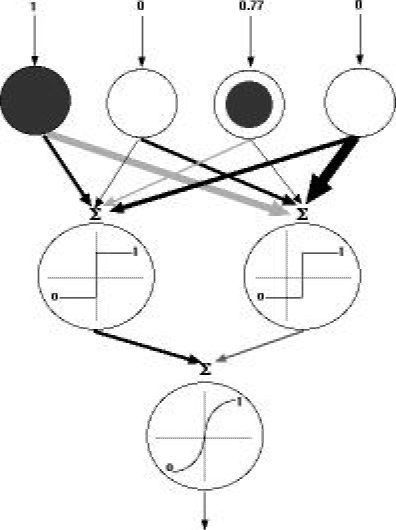
\includegraphics[width=0.55\linewidth]{section04-opponentmodel/figures/simple-neural-network}
\caption{Simple neural network example (from \cite{Davidson2002})}
\label{fig:simple-neural-network}
\end{figure}

Figure \ref{fig:simple-neural-network} shows a basic neural network, with the four input nodes on the top, two internal nodes (one hidden layer) in the middle, and the single output node on the bottom. Weights are represented by the thickness of the connection.

In this example, the internal neurons use a discrete threshold function to decide their outputs, but the output neuron uses a sigmoid function to decide its output. The two input neurons have different thresholds for firing. This is known as a bias, and each neuron can have a positive or negative bias affecting its behaviour.


\subsubsection{Backpropagation}
To "learn" these weights, a algorithm called back-propagation is used. With back-propagation, the correct answer of a training instance is worked backwards through the neural network, starting from the output and ending back at the input. The output on node $i$, $O_i$ is compared to the correct answer (the correct classification) to calculate the network's error $E_i$. Starting with the weights at the output nodes, the weights are adjusted until the error $E_i$ is minimized. Each weight is adjusted proportionally to its contribution to the error.

To calculate the contribution to the error for a connection $W_j,i$ from a internal node $j$ to an output node $i$, the error at the output node $E_i$ is multiplied by the derivative of the activation g along the input value $I_i$ to the node.

	\begin{equation}
	\Delta_i = E_i \ast g' I_i
	\end{equation}

This equation determines both the direction of the error, as well as the influence of a specific weight to the error. The weight is updated by adding $\Delta_i$ times the activation level ($O_j$ ). To adjust the amount of chance, a learning rate is applied to increase or decrease the amount of change made to the weight for each training example. The higher the learning rate, the faster the network adjusts, but the longer it takes to reach a stable condition.

	\begin{equation}
	W_{j,i} \Leftarrow W_{j,i} + \alpha  \ast O_j  \ast \Delta_i
	\end{equation}

After updating the weights at the output layer, the error is propagated further up the network. To calculate the error at an internal node connection, the following equation is applied.


	\begin{equation}
	\Delta_j = g' I_j \sum_i W_{j,i} \Delta_i
	\end{equation}

With each additional training example, the error in the network is determined and the
weights are modified using this  method. After several training iterations, the network starts to converge to a set of weights that minimize the error over all examples in the
training set. To additionally stabilize the back-propagation progress, most algorithms additionally try to minimize the error over multiple samples by reseting the network to a earlier state, should the new weights result in a weaker accuracy.

Further refinements for back-propagation algorithms are explained in in \cite{Russell2003}, \cite{Witten2005} and \cite{Rumelhart1986}. 

\subsubsection{Poker Neural Nets}
\cite{Davidson2002} trained a standard multi-layer perceptron (also known as feed-forward neural net) on contextual data collected from online games against human opponents. His network contain a set of eighteen inputs corresponding to properties of the game context, such as number of active player (his program - \texttt{Poki} - was built for ring games), texture of the board, opponent's position, the full list is shown in table \ref{fig:poki-input-nodes}.

\begin{table}[!ht]
  \begin{tabular}{ l|c | l}
\textbf{\#} & \textbf{Type}�& \textbf{Description}�\\
 \hline
 0  & real & immediate pot odds\\
 1 & real & bet ratio: \textit{bets/(bets+calls)} \\
 2 & boolean & committed (has put money in the put this round) \\
 3 & boolean & one bet to call \\
 4 & boolean & two or more bets to call \\
 5 & boolean & betting round = turn \\
 6 & boolean & betting round = river \\
 7 & boolean & last bets called by player > 0  \\
 8 & boolean & player's last action was a bet or raise \\
 9 & real & 0.1*numPlayers \\
 10 &boolean & active players is 2 (heads-up) \\
 11 & boolean & player is first to act \\
 12 & boolean & player is last to act \\
 13 & real & estimated Hand Strength for opponent \\
 14 & real & estimated Hand Potential for opponent \\
 15 & boolean & expert predictor says they would call \\
 16 & boolean & expert predictor says they would raise \\
 17 & boolean & Poki is in the hand \\

 \end{tabular}
 
\caption{Poki neural network input nodes \cite{Davidson2002}}

\label{fig:poki-input-nodes}
\end{table}

The output layer consists of the possible actions an opponent might take (this version of \texttt{Poki} was built for limit-poker, so theres only three possible actions: fold, call or raise). By graphically displaying the relative connection strengths, it's possible to determine which input parameters have the largest effects on the output. After observing networks trained on many different opponents, it is clear that certain factors are dominant in predicting the actions of most opponents, while other variables are almost completely irrelevant (\cite{Davidson2002}).

The inputs encode the knowledge of the player about the game context. All inputs are encoded to values between zero and one. The current betting round for example is encoded using two boolean input. On the flop, both inputs \#5 and \#6 are zero, if it is the turn, \#5 is set to one, and so on. \cite{Davidson2002} has also included additional expert information about the current context. Input \#13 and \#14 are the estimated hand strength - something which isn't necessairy to know with the miximax-algorithm explained in chapter \ref{c:imperfectinformation}. Inputs \#15 and \#16 indicate what an expert-buildet formula based system would do in this context. 

Figure \ref{fig:poki-neural-network} shows a resulting neural network from \cite{Davidson2002} after a few hundred hands trained from plays by a particular opponent. 


\begin{figure}[!ht]
\centering
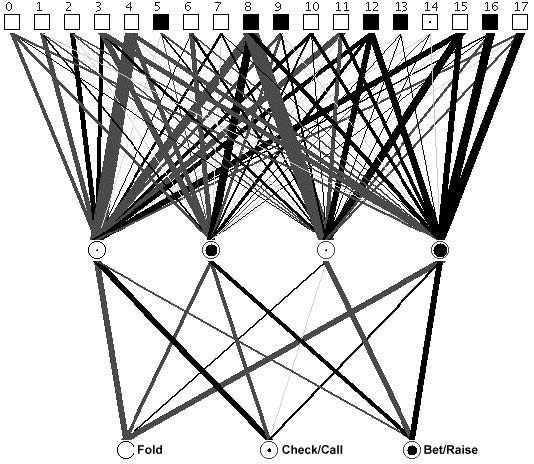
\includegraphics[width=0.7\linewidth]{section04-opponentmodel/figures/poki-neural-network}
\caption{The resulting neural network for Poki \cite{Davidson2002}}

\label{fig:poki-neural-network}
\end{figure}

The inputs are on the top, with the activation level painted as black dots, ranging from zero to one and the thickness of the lines representing the weights (black being positive, grey being negative). In this example, as \cite{Davidson2002}  explains, the connections from the input for representing a raise as the last action can be seen as very heavy, indicating a high correlation between a raise and what the opponent will do next. The outputs show that the network is predicting that the opponent will most likely bet again, with a small probability of checking. This makes intuitive sense - if a player has just bet, there is a very small chance they will fold, and a much larger chance that they will call or raise. 
Examining the graphical representations of neural networks reveal the features that have the highest correlations with the opponents actions. \cite{Davidson2002} mentions that very strong correlations could differ significantly between specific opponents. Some might be more tempted to continuation bets, putting significance on a stringent betting line, while other players actions correlate more with the texture of the public board.

Later on, \cite{Davidson2002}  used these insights to add the player's last
action to the context of the action frequency statistics. This reportedly improved
the accuracy of the statistics by an additonal 10-to-20\%.

Overall, \cite{Davidson2002} came to the conclusion, that the biggest drawback with neural networks is that they aren't trained on a proper probability distribution, but the actual event. For this reason, they don't output a distribution which is skewed to the most possible outcome and not the most accurate distribution. Nevertheless, they allow a much deeper evaluation, since the underlying logic can be graphically illustrated and analyzed. Wrong learning tendencies can be recognized and avoided this way. 


\subsection{Decision Trees}
Decision trees are another well known way to solve classification problems. Nodes in a decision tree involve testing a particular attribute. In general, the test at a node compares an attribute value with a constant. Leaf nodes give a classification that applies to all instances that reach the leaf, or more suitable for poker, a probability distribution over all possible classifications. A unknown instance is routed down the tree according to the values of the attributes tested in successive nodes, and when a leaf node is reached, the sample (or instance in the data mining framework explained later on) classified according to the class assigned to that specific leaf. 

\begin{figure}[!ht]
\centering
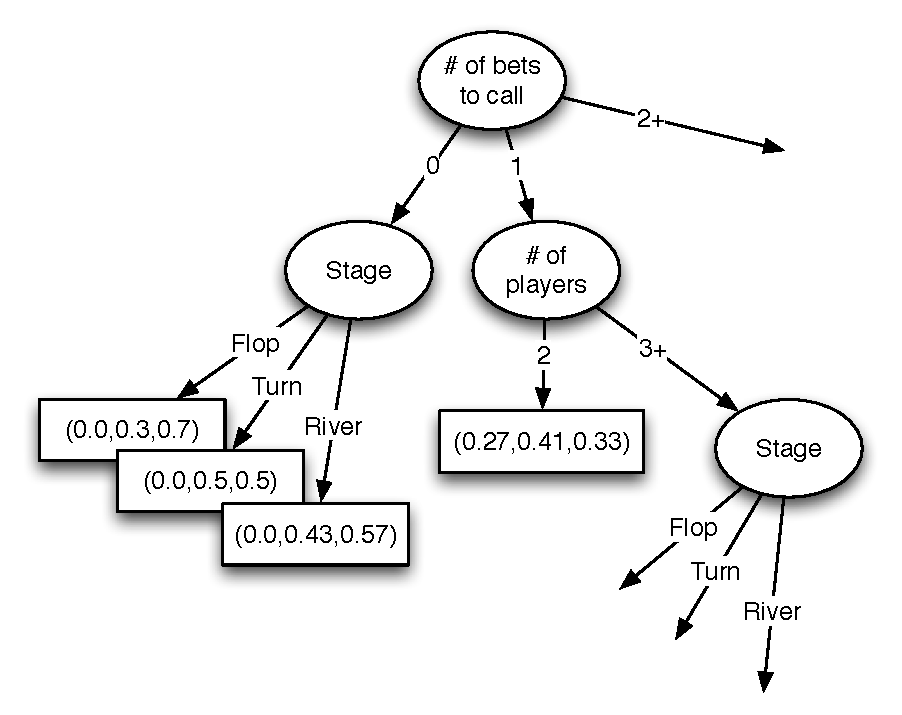
\includegraphics[width=\linewidth]{section04-opponentmodel/figures/decision-tree}
\caption{A possible decision tree example (used in \cite{Davidson2002})}
\label{fig:decision-tree}
\end{figure}

\cite{Davidson2002} used a Decision Tree Induction software \cite{Utgoff1989} to study decision trees for action prediction. Due to the high amount of noise in poker, they opted to train with tree pruning. Unfortunately, even trees with pruning activated were not as noise-tolerant as neural networks. Still, they have shown several benefits. They can output accurate probability distributions over the available choices, something neural networks can't do (as seen in the last chapter, neural networks are much better predicting the correct action than producing an accurate distribution).
Decision trees share the benefit of human readability with neural networks. They easily be represented in a very human-understandable format, although in poker this might only be of use in the debugging stage and isn't of much use once the abstraction of the contexts and the learning parameters have been fixed.

\cite{Davidson2002} concludes, that decision trees are not as accurate as neural networks, but are still a interesting avenue for further exploration.

\subsection{Alternative opponent models}

 \cite{Ponsen2008} explored an interesting bayes-relational opponent modeling system that predicts both actions and outcomes for human players in the game of No-Limit Texas Hold�em poker. His approach uses two models.  One model - the prior - is trained offline, based either on past games or some optimal values derived from equilibria calculations. 

Then, during a game, instead of updating this prior during the game, his systems learns a second model during the game, which specifies a distance function to the prior.

An action in \cite{Ponsen2008}�is viewed as an example consisting of tuple $(i,p,a_i,r_p,H_{i-1},B_i)$ of the action $a_i$ performed at stage $i$ by a player $p$, together with the outcome $r_p$ (outcomes can either be a fold before the end of the hand, a win without showing hands or showing a certain pair of cards), the the board $B_i$ and the betting history $H_{i-1}$.

He then considers the mixture $D_{p+\ast}$ of two distributions: the distribution $D_\ast$ of randomly drawn tuples from all players (the data available to the prior) and the distribution $D_p$ of randomly drawn examples from a specific opponent (say the observations in the game so far).

A theoretic learning problem then is to predict whether a randomly drawn tuple $x$ originated from $D_\ast$ (the general observations) or from $D_p$ (the distribution of the current opponent).  For a given learning setting (either predicting actions from outcomes or predicting outcomes from actions), according to \cite{Ponsen2008}�it then is easy to generate examples from $D_\ast$ and $D_p$, labeling them with $\ast$ or $p$ and learning the function $P(D_p|x)$, giving for each example the probability the observation originates from the distribution of the current opponent. 

With such a learned differentiating model, \cite{Ponsen2008}�is able (after some transformations) to formulate the final predictor 
\begin{equation}
	 P(x|D_p) = \frac{P(x|D_*) \cdot P(D_p|x)}{1-P(D_p|x)}
\end{equation}

$P(x|D_{\ast})$ being the learning prior and $P(D_p|x)$ the differentiating function. To predict a distribution of actions, one would simply create the possible tuples at the current game context and calculate the probability for each of them being part of the players set of action tuples.

To calculate the prior $P(x|D_{\ast})$ \cite{Ponsen2008}�also applies this approach to learning a differentiating function between a uniform function and the distribution formed by all examples from all players in a generic dataset.

Unfortunately, common data mining frameworks like \textit{Weka} do not support such algorithms, and the relational probability learning used by \cite{Ponsen2008}�isn't freely available. Reportetly, this approach showed impressive learning speed which already started to improve prediction rates after as little as 200 games, which is much faster than other methods, like the ones used in \cite{Billings2006b} and \cite{Schauenberg2006} which required thousands of hands to improve.

\section{Choosing the parameters and attributes}
Before learning a classification scheme with a machine learning algorithm, the data has to be preprocessed and abstract. 
As mentioned before, no-limit poker holds virtually unlimited combinations of game factor - the same context rarely occurs twice. Two ways to represent abstracted game contexts have been shown. \cite{Billings2006b} and \cite{Schauenberg2006} use multiple context trees - or trie - to store various abstractions of the current game context. Their two extrema are the not-abstracted game context with the exact action sequence leading to the current situation, and the game context simply represented by the number of actions that have happened so far.

For more conventional classifiers as used in the \textit{Weka}�Data Mining Framework, the game context have to be represented as a dataset (specifically a relation) of tuples called instances. 
Fortunately, to build the structure of such instances, much of what had been proposed by \cite{Davidson2000} and \cite{Davidson2002} as attributes of a game context in a neural network (see  \ref{fig:poki-input-nodes}) can be reused as a basis for my own abstraction of a game context.Nevertheless, the basic abstractions can be used for our own abstraction of a game context.

The model from \cite{Davidson2002} was built be used in ring poker, includes some expert knowledge (like a prediction from an additional expert system) and is used in a different game solving algorithm, so not all attributes are usable for our model. 

After experimentation, the following attributes have shown to be a solid approximation of a game context in Heads-Up No-Limit Texas Hold'em.

\begin{itemize}
\item Obviously, the observed (or to be predicted) \textbf{Action} �or \textbf{Hand Strength} �has to be part of each instance.
\item �\textbf{Bet counts}  for both players are added as an attribute, providing a measurement of aggression so far.
\item Since, unlike in Limit Poker, the \textbf{pot size} does not necessarily correlate with the number of bets and calls, it has to be added. In Models for limit poker, this wasn't necessary, as the number of bets is already an attribute. 
\item As mentioned in the section about neural networks, there is a strong correlation between the  \textbf{previous actions} and what is done next, so they have to be part of an abstracted game context. I opted to add both the action of the acting player, as well as the now observing player which did the last action. This allows the model to learn the basic poker rules (checking isn't allowed after a bet, folding after a check is a bad move in any case).
\item To take the importance of position into consideration, there is also a boolean attribute for the fact if the acting player is currently playing on the \textbf{button position}. 
\item Obviously, the \textbf{stage of the game}� has a great influence on the actions a opponent might conduct. Since cards are always shown at the river, this attribute is redundant when predicting the hand strength of a player.
\end{itemize}�
 \cite{Billings2006b}�achieved strong playing performance without taking the board into consideration. Nevertheless, I still regarded the lack of such information a great disadvantage and added three attributes which account for the structure of the public board: 

\begin{itemize}
\item The \textbf{number of face cards} �dealt for a general assessment of the strength of the board. I initially used the hand strength (how strong a hand would be if it only played with the public cards) for this, but datasets with a count of face cards have shown better prediciton accuracy for an opponents hand strength (without any influence on the action prediction) in initial experiments.
\item The \textbf{number of cards with the same suit} �and the \textbf{number of connectors}�(hands usable to build a straight)  assess the possibility of a draw for a straight or a flush.
\end{itemize}�

\chapter{Building the opponent model}
After exploring the fundamental principles and techniques for opponent modeling and specifying a set of attributes for an abstraction of a game context, this chapter now focuses on the implementation of such opponent models.

As a basic starting point, the \textit{Weka Datamining Framework} (\cite{Hall2009}) was used. \textit{Weka} is a collection of machine learning algorithms for a variety data mining tasks. The algorithms can either be used in the accompanied application, or reused directly in a java program. \textit{Weka} also contains the necessary interfaces and data types to develop new or custom machine learning schemes.

It already includes a variety of Decision Tree and Neural Network Algorithms, which allow experimentation with the techniques outlined in the previous chapter.  And can be reused in Java programs like the final implementation of a poker agent in  chapter \ref{chap:implementation}.

\section{Aquiring a Training Dataset}
Before focusing on the algorithms, a training dataset has to be acquired. I have chosen to use the large (and free) dataset of the past matches in the \textit{The Annual Computer Poker Competition}. \textit{The Annual Computer Poker Competition} is a recurring competition of the current state of the art achievements in computer poker. Each year held during a artificial intelligence conference, it's objective is to "\textit{is to benefit artificial intelligence by promoting, aiding, and evaluating research in computer poker}." Besides providing interesting results, this competition also produces a huge log of hundreds of thousands hands played. I used these logs (\cite{Hawkin2009}) to extract all game context  observed by different players during the game and their responses to them. Unlike hand histories from other sources like online poker sites, this data is free and provides hundreds of thousands of hands per opponent, instead of probably only a few hundreds per opponent. Thanks to the small number of competitions and the fact that they all matched each other in a round robin tournament, the strength of play can also be estimated. 
 
    \begin{lstlisting}[captionpos=b, caption=Example Gamestate History, label=logFile, breaklines=true]

## GAMESTATE Version 2.0
## type: DOYLE NOSTACKBOUND
# Outcomes of hand are shown in the form:
# <PLAYERS>:<HANDNUMBER>:<BETTING>:<CARDS>:<NETONHAND>
# Players are listed in seat order:big blind (or button or dealer) is listed first.
# Cards on the preflop are in seat order, divided by vertical lines |.
# The net on won or lost on a hand (in small blinds) is last, and is in seat order.
HyperboreanNL-BR|BluffBot4:0:b1b2r7c7/r81f:Kh2d|5dJs/9h4c3s:7|-7
BluffBot4|HyperboreanNL-BR:1:b1b2c2c2/c2r41f:7s5h|3sAh/9d8d4h:-2|2
HyperboreanNL-BR|BluffBot4:2:b1b2r5c5/r67f:8h9c|TsQh/8d7d2s:5|-5
BluffBot4|HyperboreanNL-BR:3:b1b2c2r8c8/r22c22/c22c22/c22r36f:3d4d|QdJd/5h7cQc/4s/Qs:-22|22
HyperboreanNL-BR|BluffBot4:4:b1b2r7c7/r81f:7sKd|3c3h/Ah2h9s:7|-7
  \end{lstlisting}
 
To make these histories usable for training in \textit{Weka}, they first have to be preprocessed into the game contexts expected by the learning algorithms. Listing \ref{logFile} shows an excerpt of the first few lines of such a raw game-state history - it follows the syntax explained in \cite{Zinkevich2007}. Listing \ref{arffFile} shows the same match after preprocessing from the perspective of \textit{HyperboreanNL-BR} observing \textit{BluffBot4}. All Pre-Flop actions have been removed, since the implementation is only used on Post-Flop decisions, and the continuos chain of actions has been converted in abstracted game contexts.

  \begin{lstlisting}[captionpos=b, caption=Example ARFF Export, label=arffFile]
@relation HandActions

@attribute PlayerAction {f,k,c,b1,b2,b3}
@attribute PotSize numeric
@attribute BetCountActingPlayer numeric
@attribute BetCountObservingPlayer numeric
@attribute LastActionActingPlayer {f,k,c1,c2,b1,b2,b3}
@attribute LastActionObservingPlayer {f,k,c1,c2,b1,b2,b3}
@attribute ActingPlayerOnButton {true,false}
@attribute FaceCards numeric
@attribute DeckSuited numeric
@attribute DeckConnectors numeric
@attribute GameStage {pf,fp,tn,rv}
@attribute TotalActionCount numeric

@data
f,88,1,1,b2,b2,true,0,1,2,fp,2
k,4,0,0,k,k,false,0,2,2,fp,0
f,43,0,1,k,b2,false,0,2,2,fp,1
f,72,1,1,b2,b2,true,0,2,2,fp,2
b2,16,2,0,b2,c2,false,1,2,0,fp,2
  \end{lstlisting}
  
For each contestant, a few million actions and hundreds of thousands of hands were extracted from the hand histories of the competition in 2009. These could then be used to both build opponent models or benchmark them.
 
\section{Updateable Data Mining Algorithms}

Building a generic opponent model from historic data is only the starting point for a good model of a poker player. After this, the model needs to be updated to the specific opponent currently playing against a player. Learning a generic opponent model a player teaches the groundwork to deduce effective poker strategies by searching the game tree. But as stated before, playing the right move only guarantees not loosing the game. To win, the player has to exploit specific style of the current opponent. This requires the opponent model to be adjusted during the game, not only to the current opponent, but also to the style he currently employs, as is common for top human players to radically change their style of play many times over the course of a match. 

This must be an ongoing process, since we may need to keep up with a rapidly changing opponent. All in all, there are a two important of requirements such a data mining algorithm needs to fulfill to be usable in the context of a poker program: 

\begin{enumerate}
	\item I must be updateable online, after having trained as a default model with batch processing. The faster it adapts the better, but it still should stay robust over the course of a game.
	\item Classification must be as fast as possible. As each decision requires a game tree of hundreds of thousands of decision nodes and showdown nodes, classification at each such node can only take a fraction of a millisecond.
	\item Nominal Classification must be supported. Both action as well as hand classification require an algorithm which can output a distribution over different nominal classes.
\end{enumerate}

After having prepared both datasets for action and hand prediction, we can train our predictor. To do this, we need to decide which learning algorithms shall be used. After some explorative experimentation with \textit{Weka}, I focused on two algorithms which will be explained in the next section and benchmarked later on.

Later exchanging the model in the game tree is simple and could possibly even be done at runtime - as long as they all implement the required interfaces found in \textit{Weka}.

\textit{Weka} 3.7 (the current developer-version) comes with 13 Classifiers which implement \texttt{UpdateableClassifier}, 14 including \texttt{BayesNet} which doesn't implement the interface, but comes with a method to update the classifier on a per-instance basis. Only a small number of these though fulfill the criteria specified above. 

Some don't allow nominal classes (e.g. Winnow), and some (most of the lazy classifiers) are simply too slow. Unfortunately, none of the the decision trees in \textit{Weka} are upteable online. 

I therefore added two additional algorithms: Hoeffding Trees from \textit{MOA}, a sister project of \textit{Weka} dedicated to online analysis of massive data streams, and an Online Learnable Perceptron from the (no longer maintained) \textit{\textit{Weka}classalgos} project.

The simple statistic methods used in \cite{Schauenberg2006} and \cite{Billings2006b} aren't implemented or benchmarked here. Unfortunately, there also is neither exact specification for a reimplementation nor specific performance data (in terms of prediction accuracy) which would allow comparison to the methods used here. The only thing that can be derived from the publicized data of the programs using these models, is that they require tens of thousands of hands of online training to break even against top opponents.

\subsection{Online Backpropagation}

To update a multilayer perceptron during a match, batch learning of a network can't be used. Fortunately, the same formulas as in normal backpropagation can  be used to update the weights incrementally after each training instance has been processed. 

\cite{Witten2005}�calls this stochastic backpropagation because the overall error does not necessarily decrease after every update and there is no guarantee that it will converge to a minimum. 

After experimenting with my own extension of \textit{Weka}'s Multilayer Perceptron, but without achieving any satisfying results, the Back-Propagation Algorithm from the \textit{Weka Classification Algorithms} project was applied. Based on the algorithms in \cite{Reed1998}�it implements a basic feed-forward artificial neural network with an adaptable number of layers, momentum and decay and provides an online learner which allows iterative updating of the network. 

As the benchmarks at the end of this chapter will show, this algorithm at least occasionally resulted in stable learning behavior.

\subsection{Hoeffding Tree}


Hoeffding Trees are a decision tree based approach by \cite{Domingos2000} for classifying high speed data streams. These streams share a common ground with the classification requirements in a game tree. Hoeffding Trees not only promise fast classification, but also stable updateability.

The induction algorithm used in Hoeffding trees induces a decision tree from a data stream incrementally, briefly inspecting each example in the stream only once, without need for storing examples after they have been used to update the tree. 

The only information stored in memory is the tree itself, which stores enough information in its leaves in order to grow, but also classify instances between updating from new instances. The resulting trees still provide classification almost as good as a tree learned by batch learning (though online learning will never be able to surpass batch learning).

\subsubsection{Hoeffding Tree Induction}
As usual in a decision tree, each node in a Hoeffding Tree contains a test to divide the instances along different paths depending on the values of a particular attribute. The crucial decision is when building a decision tree is when to split a node, and with what test condition this split should be executed. If the tests used to divide examples are based on a single attribute value, as is typical in classic decision tree systems, then the set of possible tests is reduced to the number of attributes. In this case, the problem becomes a simple selection of the right attribute to split on. 

To find these tests, well established criteria like the measure of information gain in the C4.5 algorithm have become popular. This measures the increase in entropy gained by the tree below a split. To calculate the information gain, the weighted average of the subset of a split are subtracted from the entropy of the class distribution $p_n$ before splitting. Such an entropy is calculated as:

\begin{equation}
entropy(p_1,p_2,...,p_n) = \sum_{i=1}^n -p_i log_2 p_i \mbox{, where $n =$ number of classes, and } \sum_{i=1}^n p_n = 1
\end{equation}
\cite{Bifet2009}

In a batch learning setting, estimating the information gain is straightforward, as one could simply choose the attribute with the highest information gain over all of the available and applicable training data. But, as \cite{Bifet2009} highlights, such an estimation is much more difficult in a online learning setting. Initially introduced by \cite{Domingos2000}, the Hoeffding Bound is proposed to make such a similar decision as in the offline learning setting.

The Hoeffding bound states that with probability $1-\delta$, the true mean of a random variable of range R will not differ from the estimated mean after $n$ independent observations by more than

\begin{equation}
\epsilon = \sqrt{\frac{R^2ln(1/\delta)}{2n}}
\end{equation}

This bound holds true regardless of the distribution of the underlying values, and relies solely on the range of the values, number of observations and desired probability. To find the attribute to split on, the random variable being estimated is the difference in information gain between the best two attributes.

For information gain the range of values ($R$) is the base 2 logarithm of the number of possible class values. With R and $\delta$ fixed, the only variable left to change the Hoeffding bound ($\epsilon$) is the number of observations ($n$). As $n$ increases, $\epsilon$ will decrease, in accordance with the estimated information gain getting ever closer to its true value.

Now, a simple test allows the decision that an attribute has superior information gain compared to others, when the difference in observed information gain is more than $\epsilon$ (with confidence $1-\delta$) - we can therefore decide to use this attribute for the splitting test. This is the core principle for Hoeffding tree induction, leading to the following algorithm (from \cite{Bifet2009}.

\begin{lstlisting}[captionpos=b, caption=Hoeffding Tree Induction \cite{Bifet2009}, label=hoeffding-algorithm, mathescape=true,breaklines=true]
Let $HT$ be a tree with a single leaf (the root)
for all training instances do:
   Sort example into leaf $l$ using $HT$
   Update sufficient statistics in $l$ and increment $n_l$, the number of examples seen at leaf $l$
   if $n_l$ $mod$ $n_{min} = 0$ and instances seen at $l$ not all of same class then
      Compute $G_l(X_i)$ for each attribute
      Let $X_a$ be attribute with highest $G_l$
      Let $X_b$ be attribute with second-highest $G_l$
      Compute Hoeffding bound $\epsilon$ = $\sqrt{\frac{R^2ln(1/\delta)}{2n_l}}$
      if $X_a \neq X_0$ and $(G_l(X_a)-G_l(X_b)$ > $\epsilon$ or $\epsilon < \tau$) then 
         Replace $l$ with an internal node that splits on $X_a$
         for all branches of the split do
            Add a new leaf with initialized sufficient statistics
         end for
      end if
   end if
end for
\end{lstlisting}
The first line simply initializes the tree data structure with a single root node. The rest of the algorithm is performed for every training example. Every example is filtered down the tree to an appropriate leaf, depending on the tests already present in the decision tree built to that point (sorting example into leaf using $HT$). 

As the next step, this leaf is then updated - each leaf in the tree holds the sufficient statistics needed to make decisions about further growth and the number of observations at this node is incremented. The sufficient statistics that are updated are those that make it possible to estimate the information gain of splitting on each attribute. 

For efficiency reasons the code block after that is only performed periodically, every $n_min$ examples for a particular leaf, and only when necessary, when a mix of observed classes permits further splitting.  During this, the test described in the previous section is performed, using the Hoeffding bound to decide when a particular attribute has won against all of the others. 

$G$ is the splitting criterion function (information gain) and its estimated value. In line 11 the test for $X_0$, the null attribute, is used for pre-pruning. The test involving $\tau$ is used for tie-breaking.
If an attribute has been selected as the best choice, lines 12-15 split the node, causing the tree to grow. 

For more in depth explanation, \cite{Bifet2009}�is refered, going into details about all tests and the required methods to keep the tree both fast and light on memory usage.

\section{Hand Prediction}

Two problems arise when predicting the value of a hand. First, we need a measurement of the strength of a hand, and second, the standard API of \textit{Weka} doesn't provide any distribution information, so a probability of a stronger hand can be approximated.

To measure the strength of a hand, a lot of different algorithms exist. The poker-eval algorithm of the Pokersource project \cite{Pokersource2009} is probably the  the most widely-used poker hand evaluator. Poker-eval is fast (thanks to using JNI, C and a lot of static lookup tables and macros) and supports most poker variants, from Hold'em to Omaha and Stud Poker. 

The first implementation of the opponent model and agent also used this algorithm. But for later versions I decided to switch to the algorithm by \cite{Suffecool2006}. 
Although a little bit slower, since completely writen in java, the advantages overweight the slowdown: 

\begin{itemize}
\item Instead of a generic number for each possible hand, with only a garantee that the higher the number the better the hand, this  algorithm provides an enumeration of all 7462 distinct hands. This way, the opponent model is much more accurate, compared to the poker-eval values, which can go in to the billions, despite the fact that there are only 2598960 possible 5card hands.
\item The pure java implementation provides an important advantage for portability. To train the opponent models based on the vast database of past hands, a 64bit JVM is required, as 32bit virtual machines barely start when using more than 1GB of ram. On the other hand, when using the actual agent, there is no need for such a large amount of ram, and since there is no  guarantee that a 64bit JVM is present, the library would also have to be compiled for 32bit. In the end, 4 different binaries would have to be maintained (assuming the program should work on both Windows an Mac OSX, both 32bit and 64bit). With a pure java implementation, this isn't necessary.
\end{itemize}

Central to the algorithm of  \cite{Suffecool2006} is the idea of associating a prime number with each card. After this a variety of bitwise operations and lookup tables are applied to map the five-card poker hand to a specific equivalence class. This equivalence class (e.g. "King-high Straight") can then easily looked up in a last lookup table. 

After being able to compute a unique value for each equivalence class of hand, one problem still remains. The Miximax-Algorithm by \cite{Billings2006b} presented in chapter \ref{c:imperfectinformation} requires a distribution over the strength of possible hands of the opponent at the leaf nodes. Unfortunately, the \textit{Weka} framework doesn't provide any distributions for numeric predictions. Some classifier enhancer are available to predict conditional densities - but unfortunately those can't be used to calculate the density over a range of values - we would need the density between zero and the strength of our hand at the leaf. To circumvent this problem, parts of these enhancers could be used to create a class which can calculate the possibility of the opponent holding a stronger hand.

The meta classifier \texttt{RegressionByDiscretization} provides a wrapper to classify a numeric attribute into different bins, making it a nominal attribute. After calculating the underlying distribution with the original classifier of the class among these bins a estimation of the distribution can be calculated.

\begin{figure}[!ht]
\centering
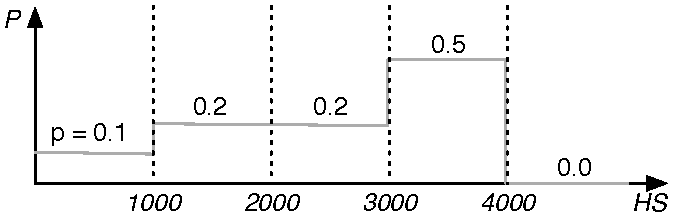
\includegraphics[width=\linewidth]{section04-opponentmodel/figures/handdist}
\caption{Possible distribution over imaginary hand strengh bins}
\label{fig:handstrength-distribution}
\end{figure}

Figure \ref{fig:handstrength-distribution} shows the basic idea used to convert the nominal prediction over the bins into the density to a certain point (the probability of hands worse than the one of the player). After having added this to our own version of \texttt{RegressionByDiscretization}, we can caclulate getPercentageHigher(Instance, double value) the number of times we would beat the opponent in such a situation.\texttt{uzholdem.classifier.hand.\textit{Weka}HandDistribution} is now able to compute the values required by the Miximax-Values, and can reuse all classifiers from both \textit{Weka} and MOA.

Assuming a player hand-strength of 2300. The probability of the opponent holding a stronger hand would be calculated as follows: $0.1 + 0.2 + 0.2 * \frac{2300-2000}{3000-2000} = 0.36$ 



\section{Quadratic Loss Function}
Measuring the quality of the opponent model, means evaluation the quality of the prediction of the model. As the game tree search assumes the opponent doesn't play a distinct action each time he encounters a specific situation, but varies his play over a certain distribution of action, it makes sense to also measure the quality of the opponent models distribution, and not only the amount of correctly predicted actions. Therefore, we use the quadratic loss function to measure the quality of the models prediction, as advised by \cite{Witten2005} for judging the quality of distributions (opposed to the information loss function, which is oblivious about the probabilites of the events not occured).

Suppose that for a single instance (or game context) there are k possible outcomes (opponent actions), and
for a given instance the learning scheme comes up with a probability vector $p_1$,
$p_2$, . . . , $p_k$ for the classes (where these probabilities sum to 1). The actual
outcome for that instance will be one of the possible classes. A second vector $a_1$,$a_2$,...,$a_k$ represents this outcome, whose ith component, where i is
the actual outcome, is 1 and all other components are 0. The penalty assosiated with this situation can now be expressed as a loss function that depends on both the prediction as the vector $p$ and the outcome as the vector $a$.
With the quadractic loss function, this penalty is calculated by 

\begin{figure}[h]
\begin{equation}
\sum_{j}(p_{j}-a_{j})^2
\end{equation}
\caption{Quadratic Loss, as calculated in \cite{Witten2005}}
\end{figure}

\section{Results}
To measure the efficiency and accuracy of the different algorithms for an opponent model, I concluded multiple benchmark. Based on the (preprocessed) hand histories from the 2009 \textit{Annual Computer Poker Competition}, different opponent models for each algorithm were created.

In 2009, five participants played in the no-limit competition. Each opponent model is benchmarked for each opponent. To do this, the algorithm is trained on all matches excluding the observations of the specific benchmark opponent. After creating, the opponent model then is updated as if it would replay as a player in each match of the benchmark opponent. 

After this, the results during the match of the adapting model were compared to the of the same model not updating during each match (the metrics for each game context are average over all benchmark matches). At the end of each match, both models were reset.

Including only the three best players, the benchmark opponents were: 

\begin{itemize}
\item \textbf{HyperboreanNL-Eqm} (University of Alberta) - winner no limit run-off, runner-up in no limt bankroll. The official competition homepage states: \textit{"Hyperborean-Eqm was created using the same techniques used by the University of Alberta as in the past, with the exception that it now uses soft translation. Additionally, the methods used to create the strategy have been further optimized for no-limit play."}
\item \textbf{HyperboreanNL-BR} (University of Alberta) - winner in no limit bankroll, runner-up in no limt run-off. Official description: \textit{ Hyperborean-BR employed a variety of techniques designed to exploit the traditional method of translation used by agents. This involves manipulating the pot size in ways that are indistinguishable to its opponent. In order to exploit its opponent, it performs exploration at the beginning of the match to create a rough model of its opponent.}
\item \textbf{BluffBot4} (Teppo Salonen) - 3rd place in bankroll and run-off. Described with \textit{"The AI (artificial intelligence) used in all BluffBot versions is a non-adaptive expert system designed using the principles of game theory. This approach makes a good practical use of variety of known expert strategies exploiting weaker opponents while at the same time effectively defending itself against exploitation from adaptive opponents."}
\end{itemize}

For both hand and action prediction, the quadratic loss was measured. In the final implementation, this is much more important than the actual number of correctly predicted actions or hands. 

Since the effort to train the classifier isn't very important (we only need to update it after each hand), the computational cost of updating the classifier wasn't benchmarked. Initial experimenting has shown that it is fast enough in all algorithms,.

\newpage
\subsection{Performance in Action Prediction: Naive Bayes}
\begin{figure}[h!]
\centering

\subfigure[Model of HyperboreanNL-Eqm: Quadratic Loss]{
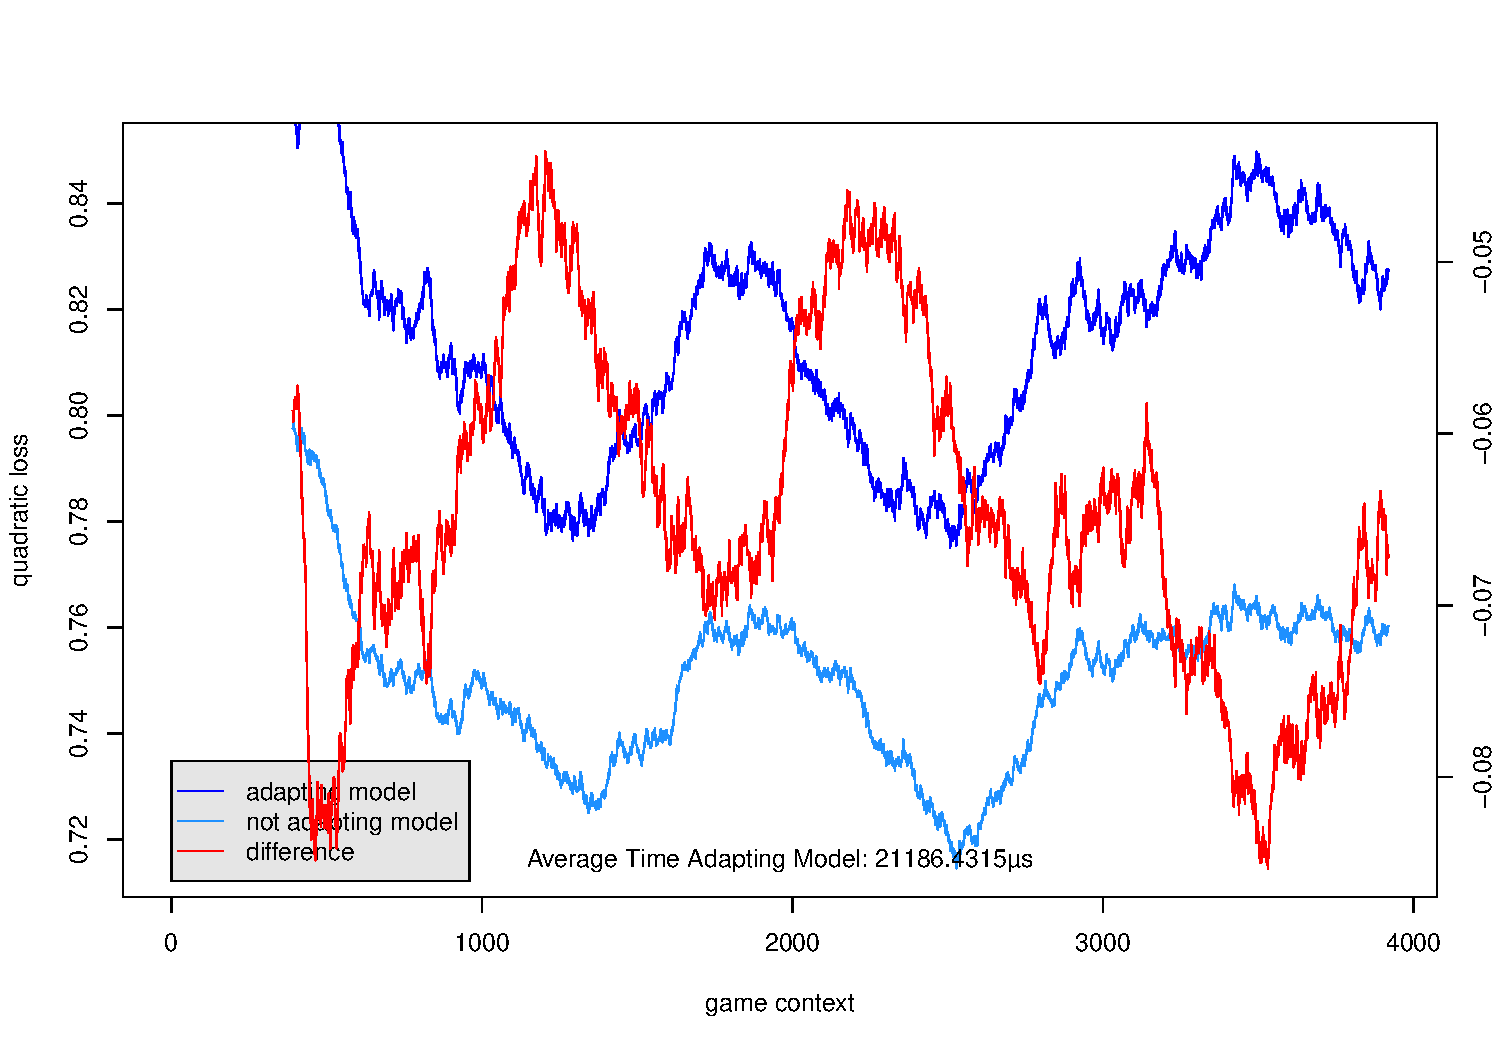
\includegraphics[scale=0.275]{section05-modelimpl/figures/MOANaiveBayes-HyperboreanNL-Eqm-action-quadratic}
}
\subfigure[Model of HyperboreanNL-Eqm: Correctly Predicted]{
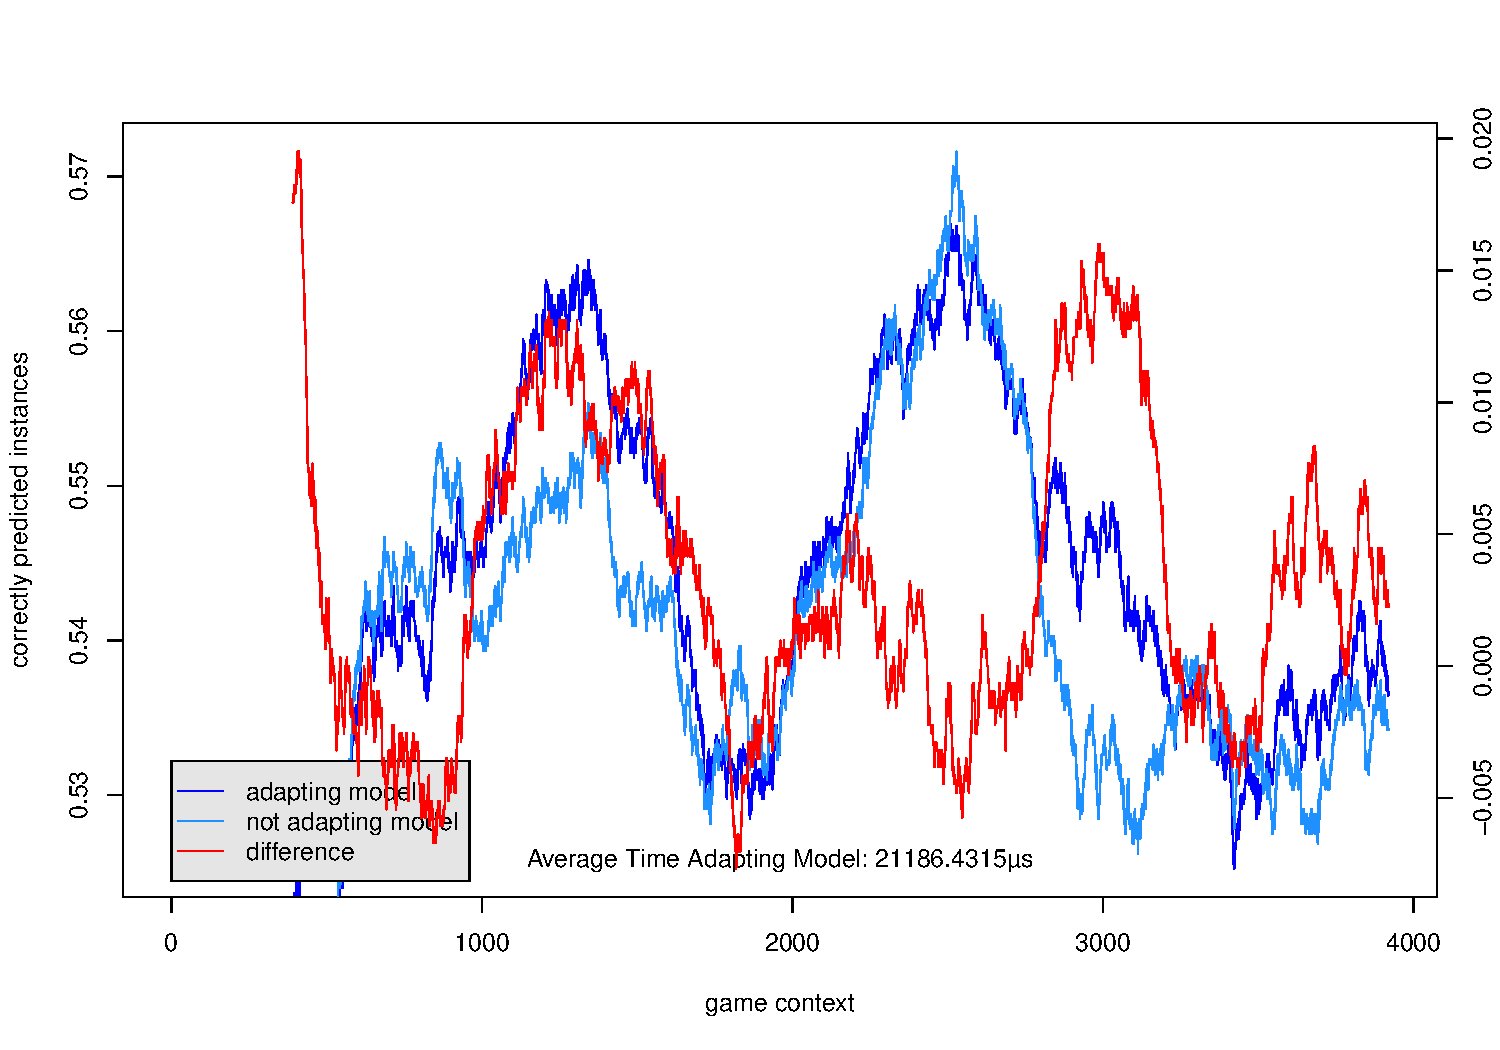
\includegraphics[scale=0.275]{section05-modelimpl/figures/MOANaiveBayes-HyperboreanNL-Eqm-action-correctly}
}

\subfigure[Model of HyperboreanNL-BR: Quadratic Loss]{
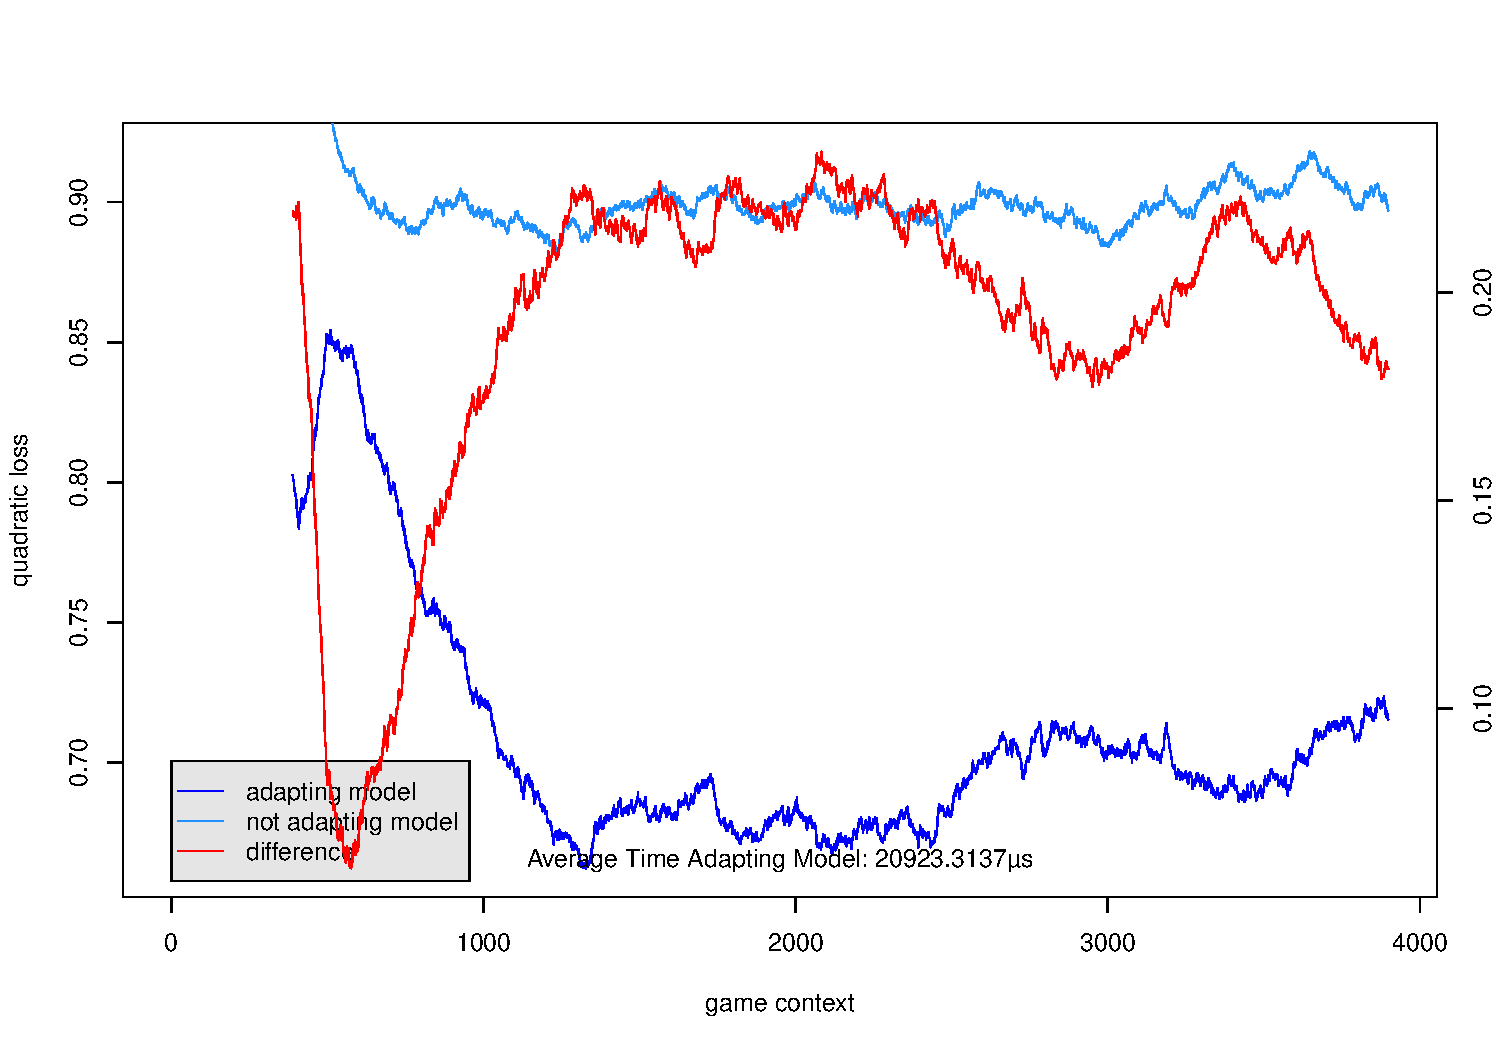
\includegraphics[scale=0.275]{section05-modelimpl/figures/MOANaiveBayes-HyperboreanNL-BR-action-quadratic}
}
\subfigure[Model of HyperboreanNL-BR: Correctly Predicted]{
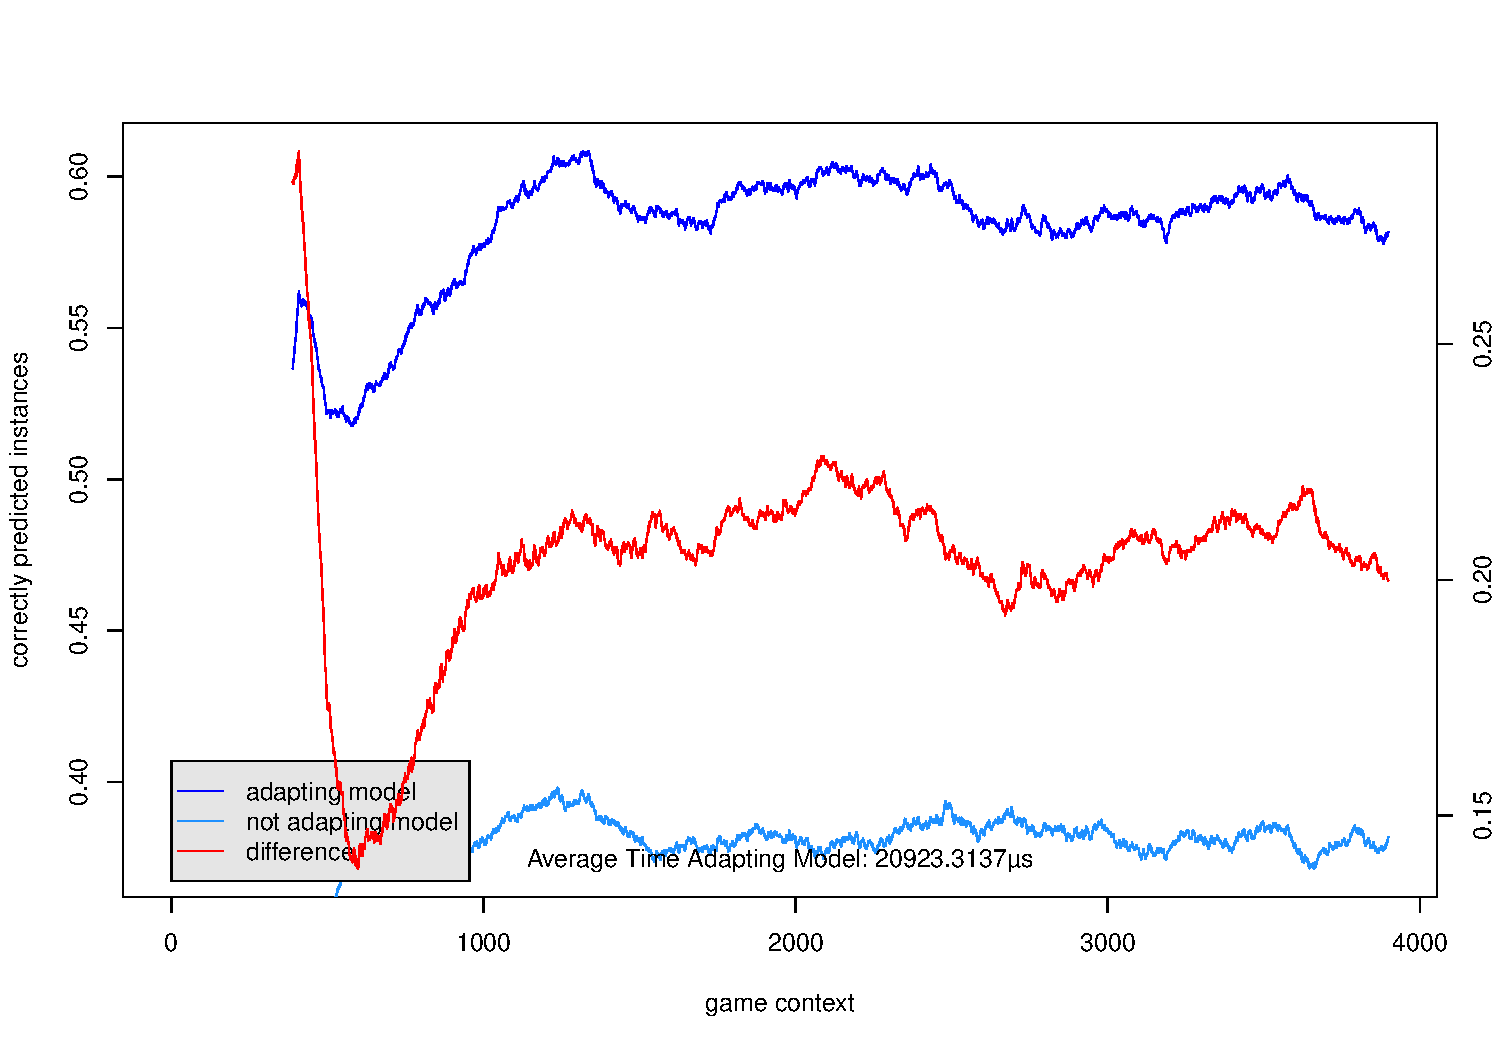
\includegraphics[scale=0.275]{section05-modelimpl/figures/MOANaiveBayes-HyperboreanNL-BR-action-correctly}
}

\subfigure[Model of BluffBot4: Quadratic Loss]{
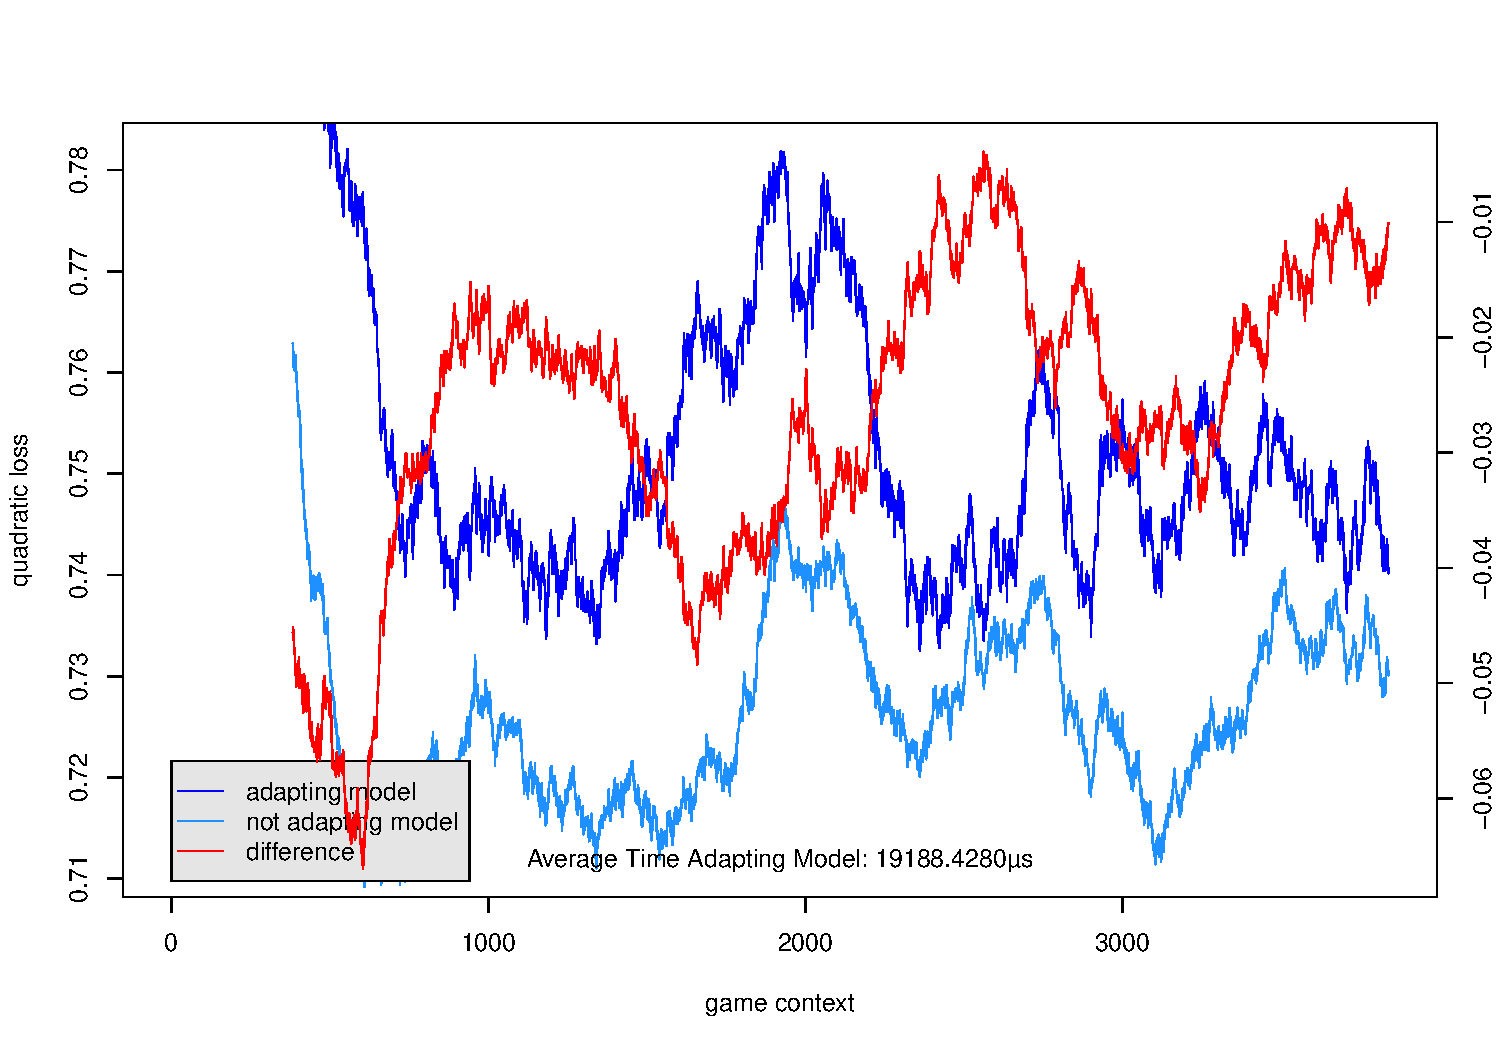
\includegraphics[scale=0.275]{section05-modelimpl/figures/MOANaiveBayes-BluffBot4-action-quadratic}
}
\subfigure[Model of BluffBot4: Correctly Predicted]{
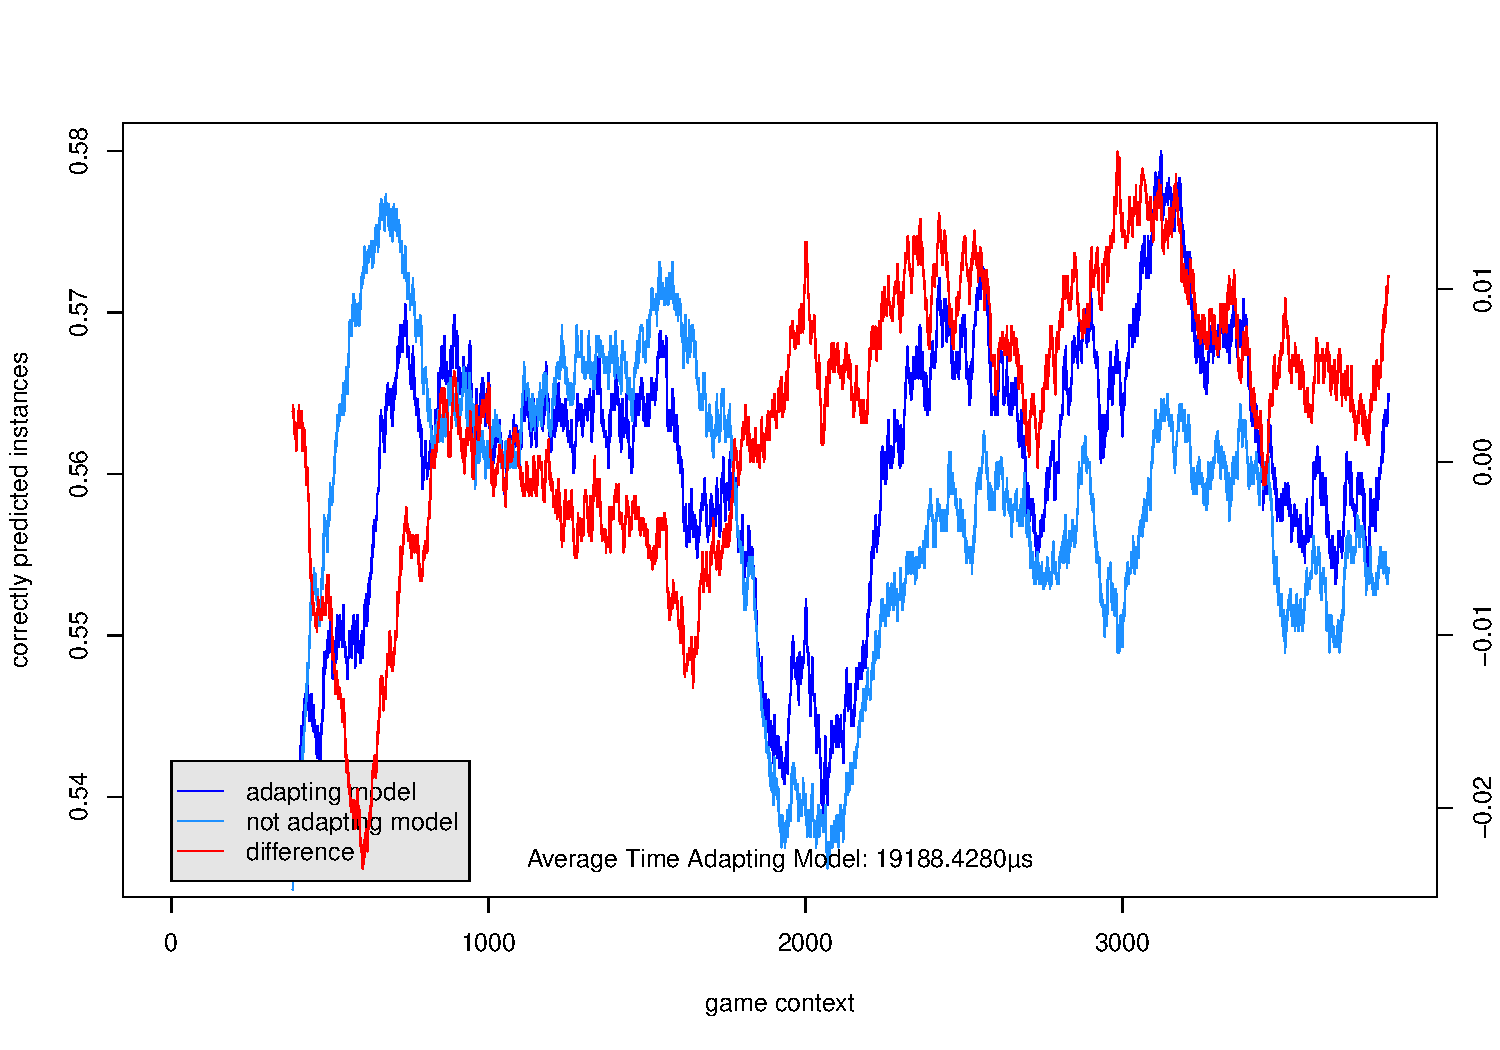
\includegraphics[scale=0.275]{section05-modelimpl/figures/MOANaiveBayes-BluffBot4-action-correctly}
}

\caption{Action Prediction: Naive Bayes}
\label{fig:MOANaiveBayes-action}
\end{figure}




\newpage
\subsection{Performance in Action Prediction: Online Backpropagation}
\begin{figure}[h!]
\centering

\subfigure[Model of HyperboreanNL-Eqm: Quadratic Loss]{
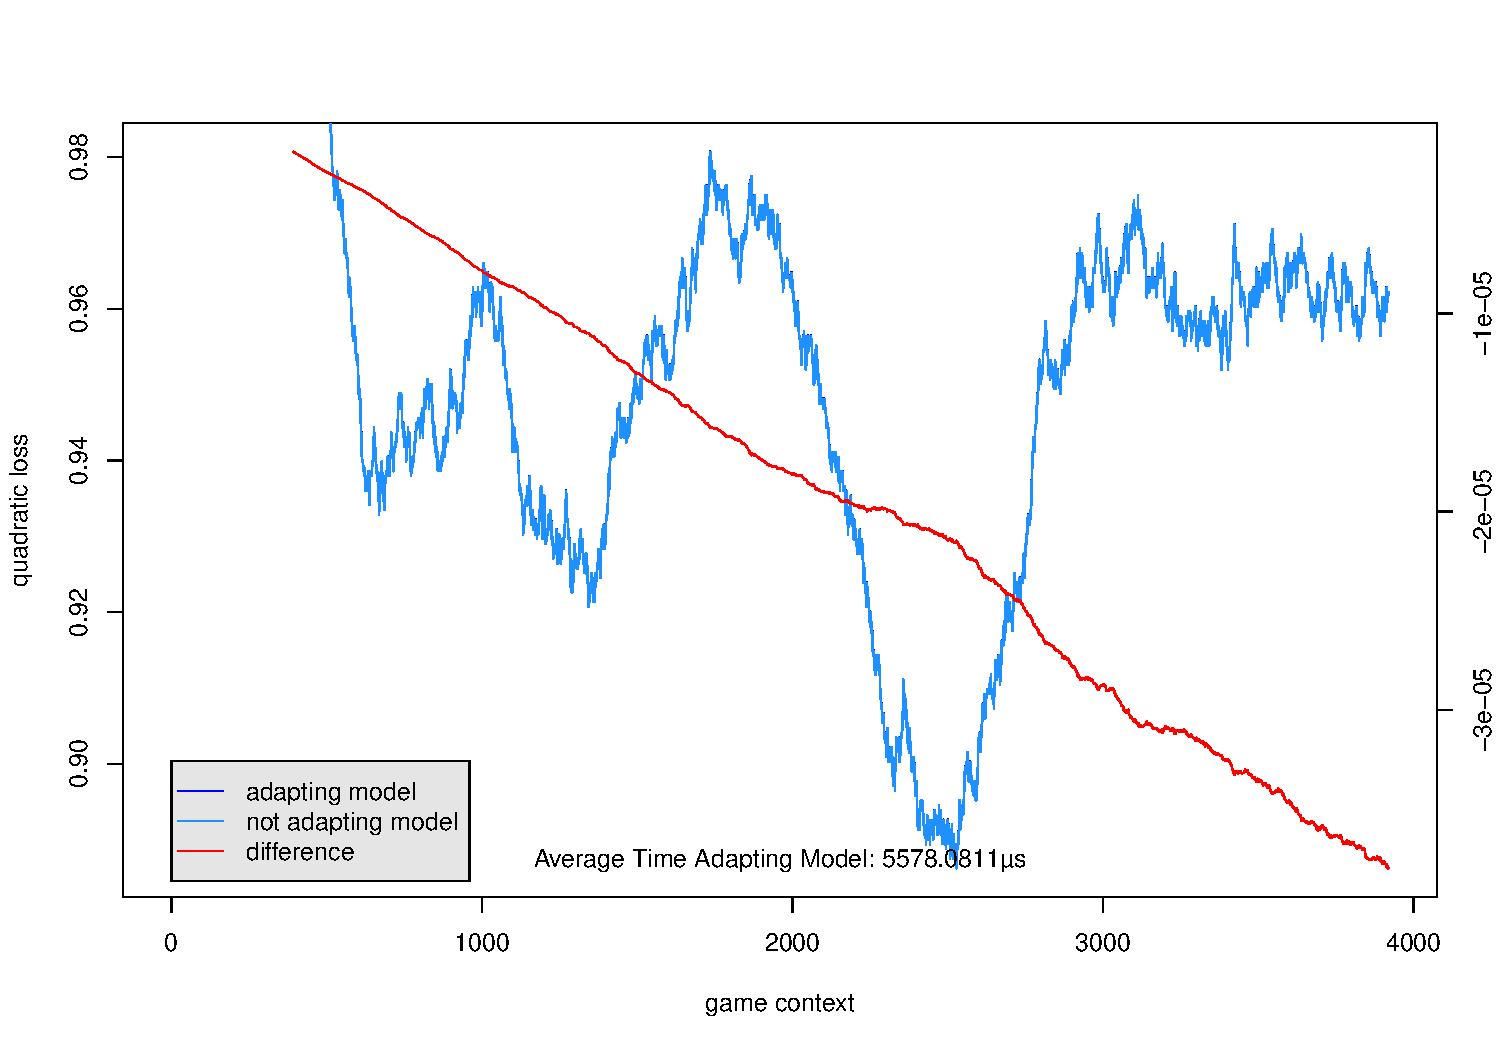
\includegraphics[scale=0.275]{section05-modelimpl/figures/OnlineBackpropagation-HyperboreanNL-Eqm-action-quadratic}
}
\subfigure[Model of HyperboreanNL-Eqm: Correctly Predicted]{
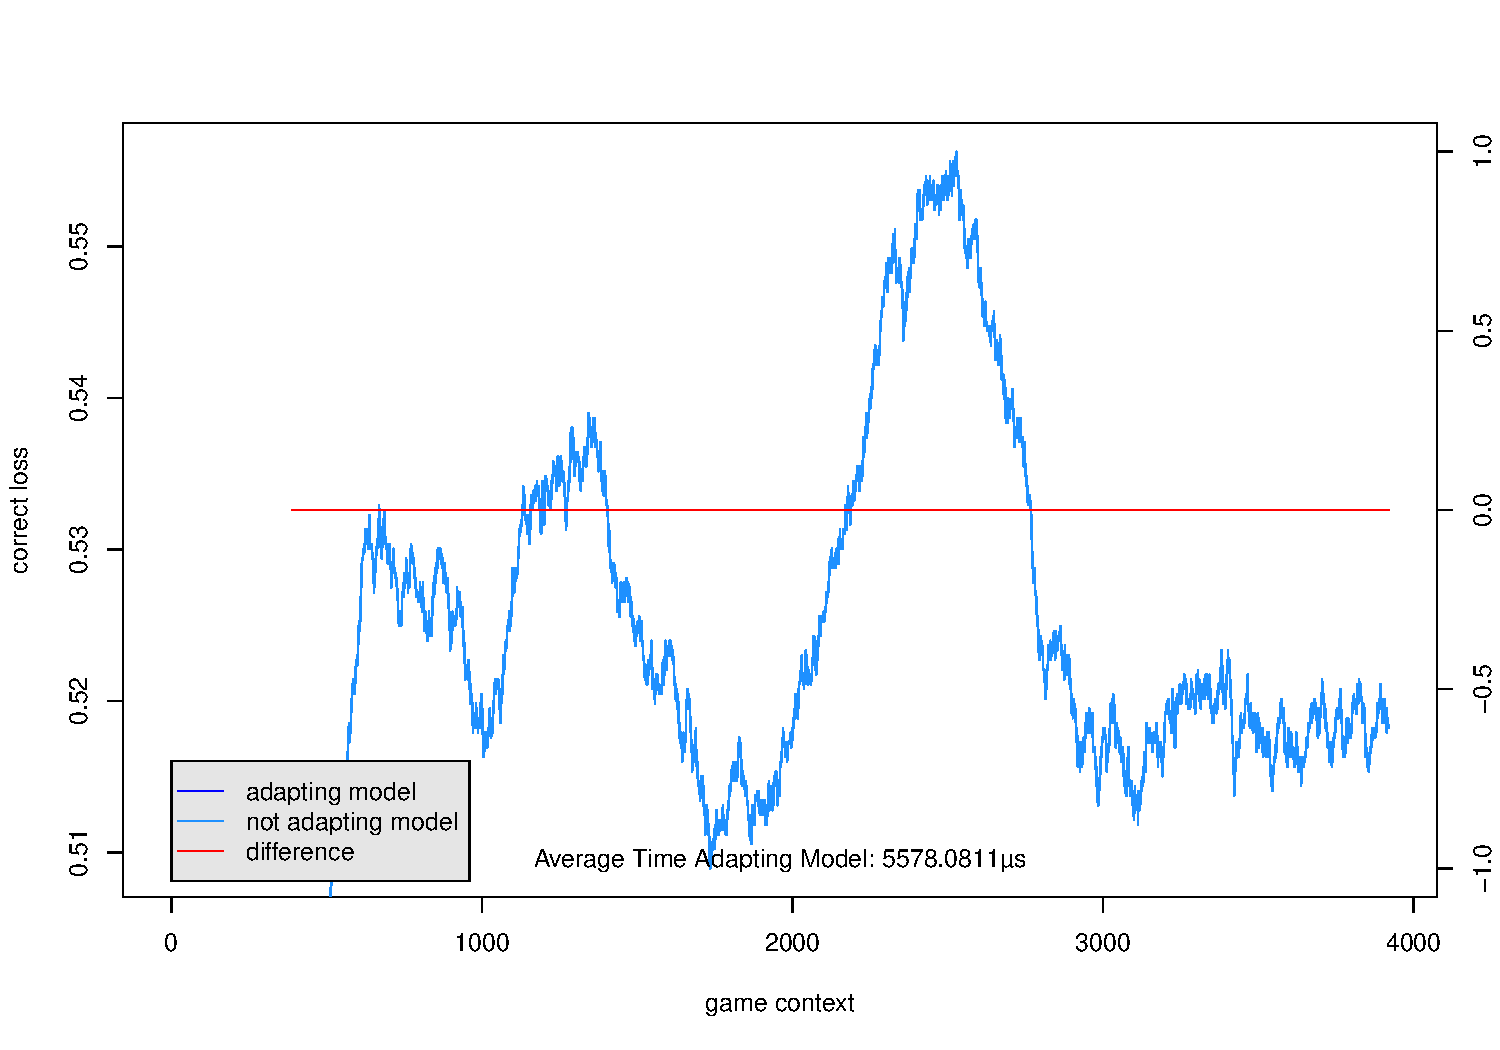
\includegraphics[scale=0.275]{section05-modelimpl/figures/OnlineBackpropagation-HyperboreanNL-Eqm-action-correctly}
}

\subfigure[Model of HyperboreanNL-BR: Quadratic Loss]{
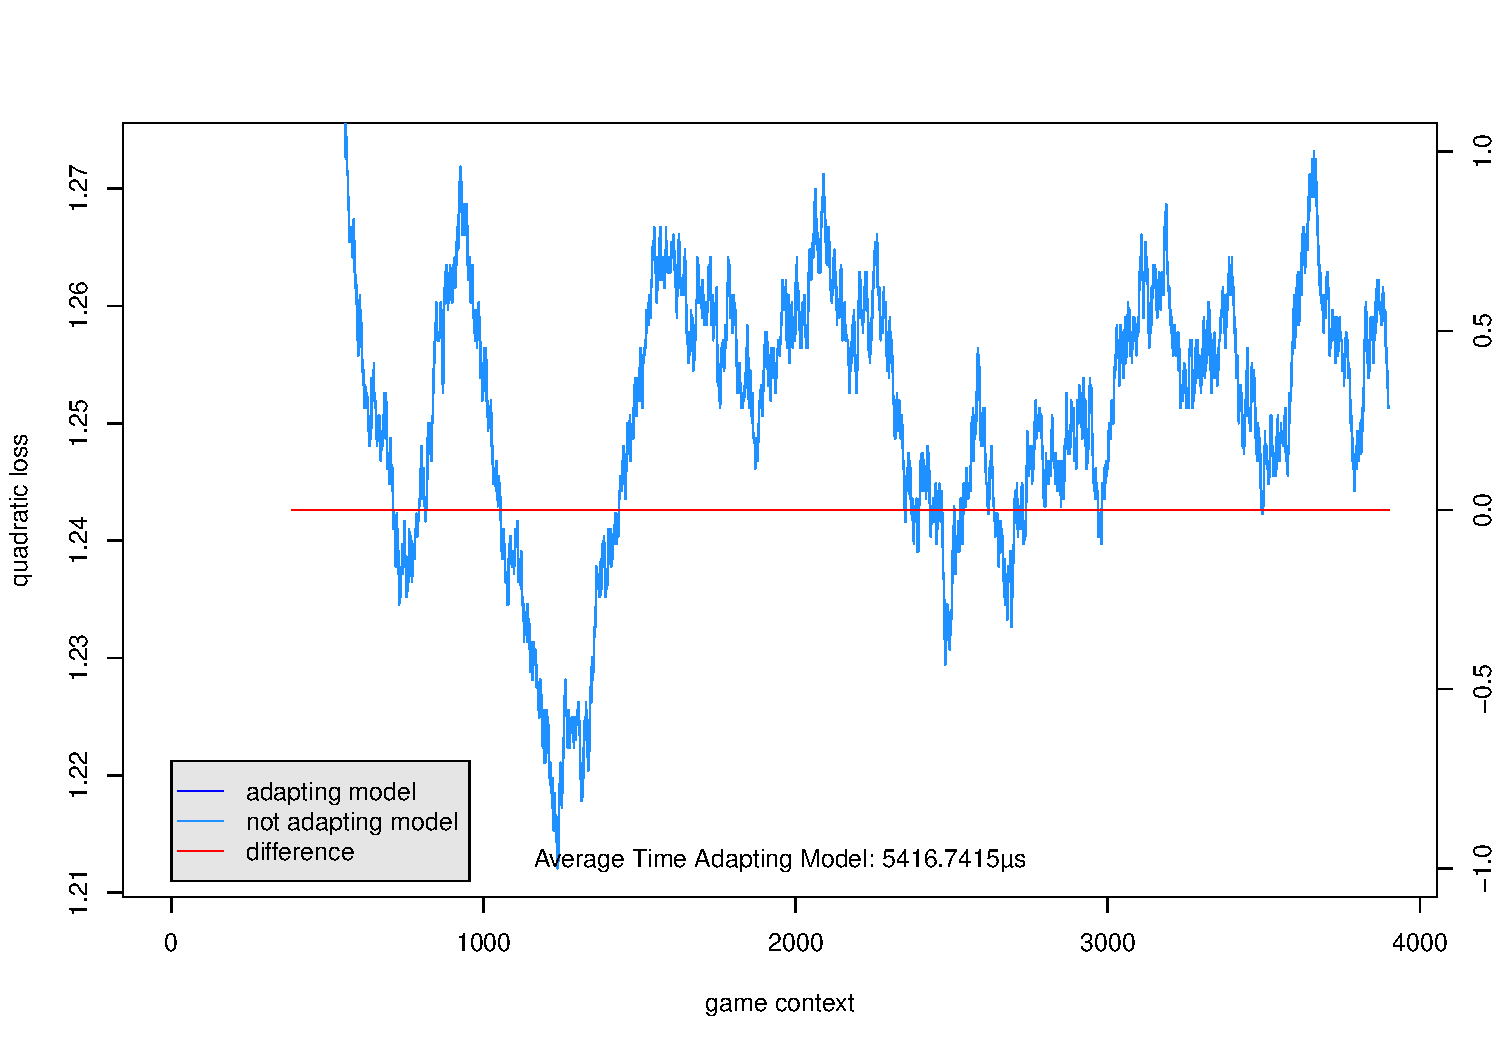
\includegraphics[scale=0.275]{section05-modelimpl/figures/OnlineBackpropagation-HyperboreanNL-BR-action-quadratic}
}
\subfigure[Model of HyperboreanNL-BR: Correctly Predicted]{
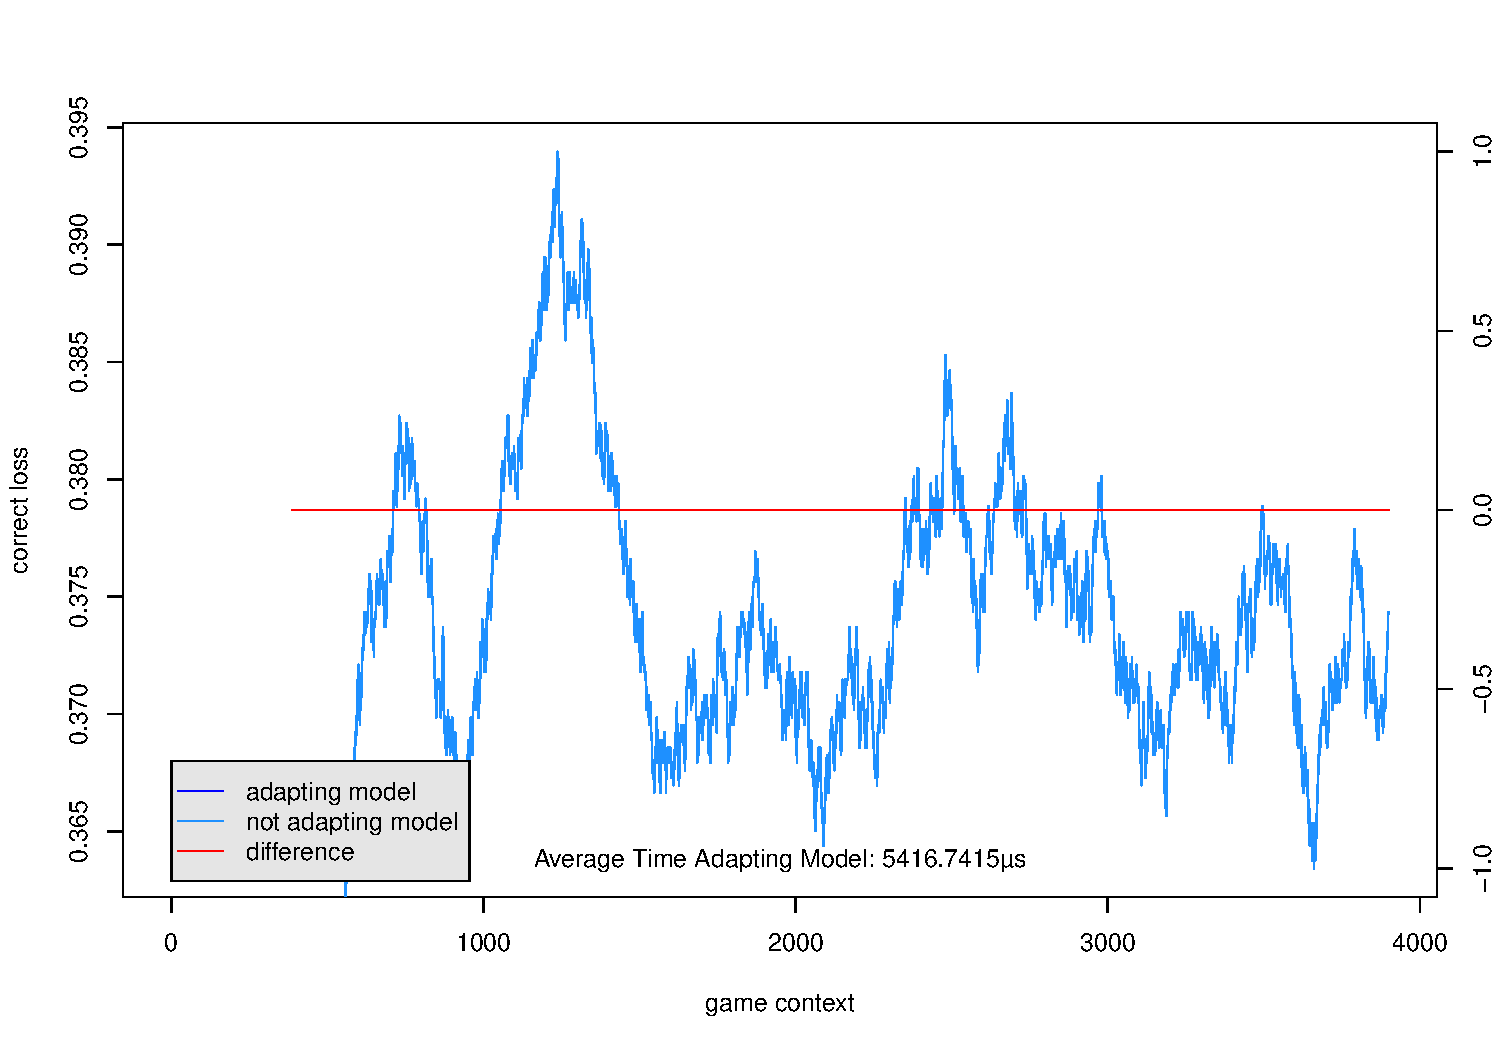
\includegraphics[scale=0.275]{section05-modelimpl/figures/OnlineBackpropagation-HyperboreanNL-BR-action-correctly}
}

\subfigure[Model of BluffBot4: Quadratic Loss]{
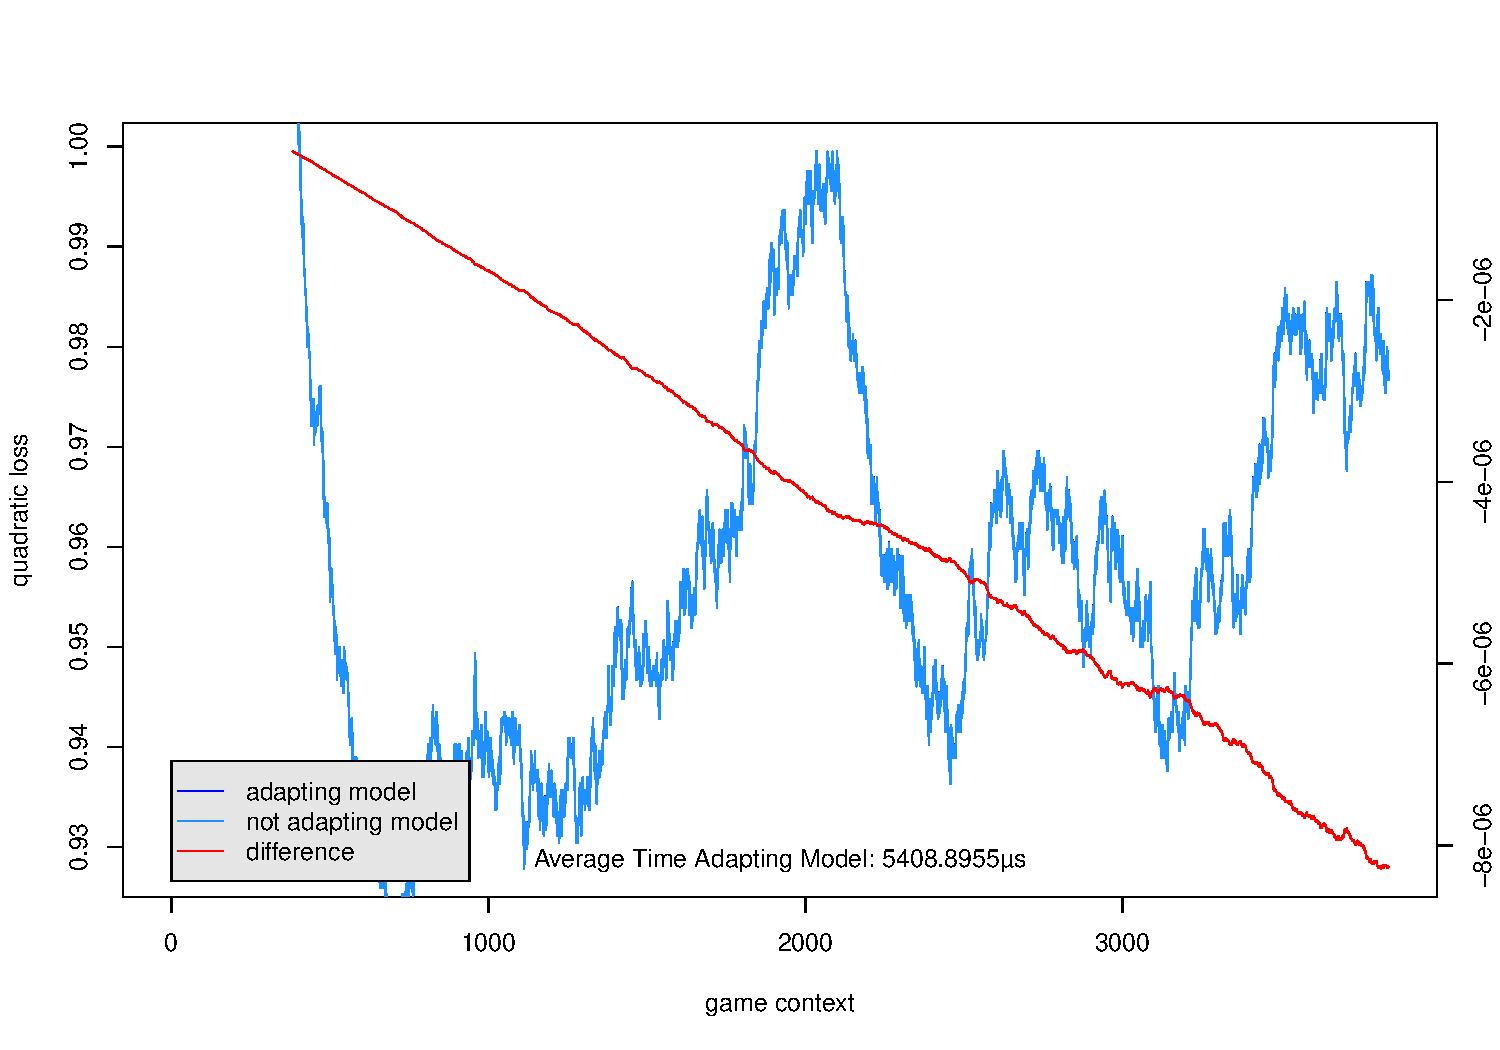
\includegraphics[scale=0.275]{section05-modelimpl/figures/OnlineBackpropagation-BluffBot4-action-quadratic}
}
\subfigure[Model of BluffBot4: Correctly Predicted]{
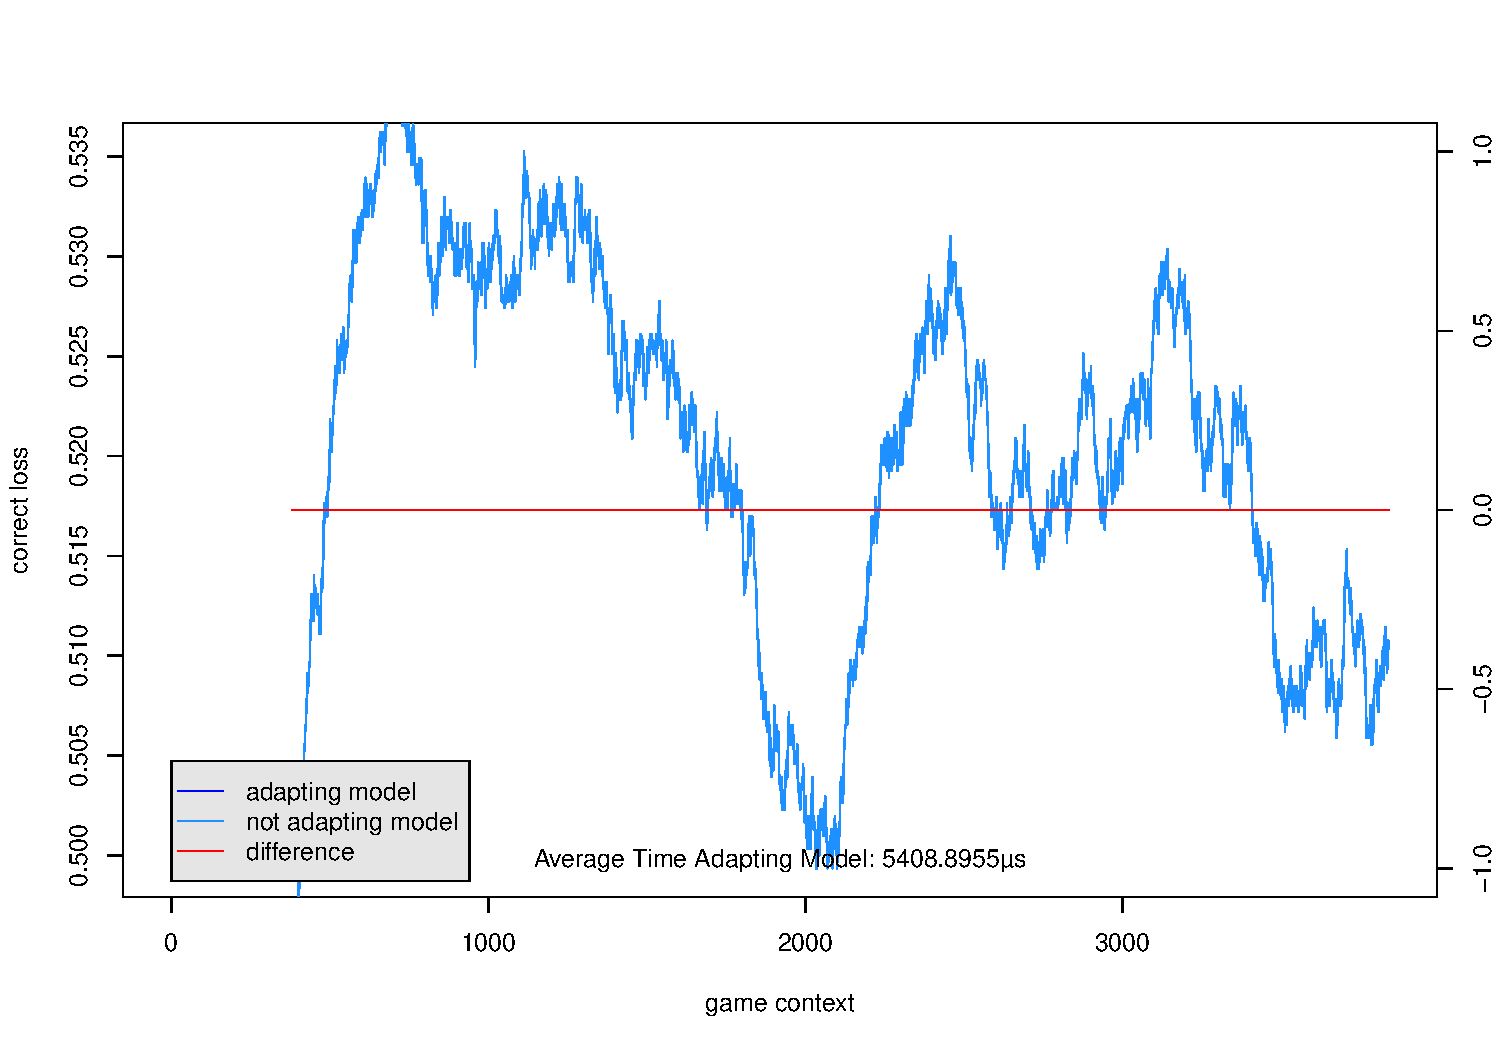
\includegraphics[scale=0.275]{section05-modelimpl/figures/OnlineBackpropagation-BluffBot4-action-correctly}
}

\caption{Action Prediction: Online Backpropagation}
\label{fig:OnlineBackpropagation-action}
\end{figure}


\newpage
\subsection{Performance in Action Prediction: Hoeffding Tree}
\begin{figure}[h!]
\centering

\subfigure[Model of HyperboreanNL-Eqm: Quadratic Loss]{
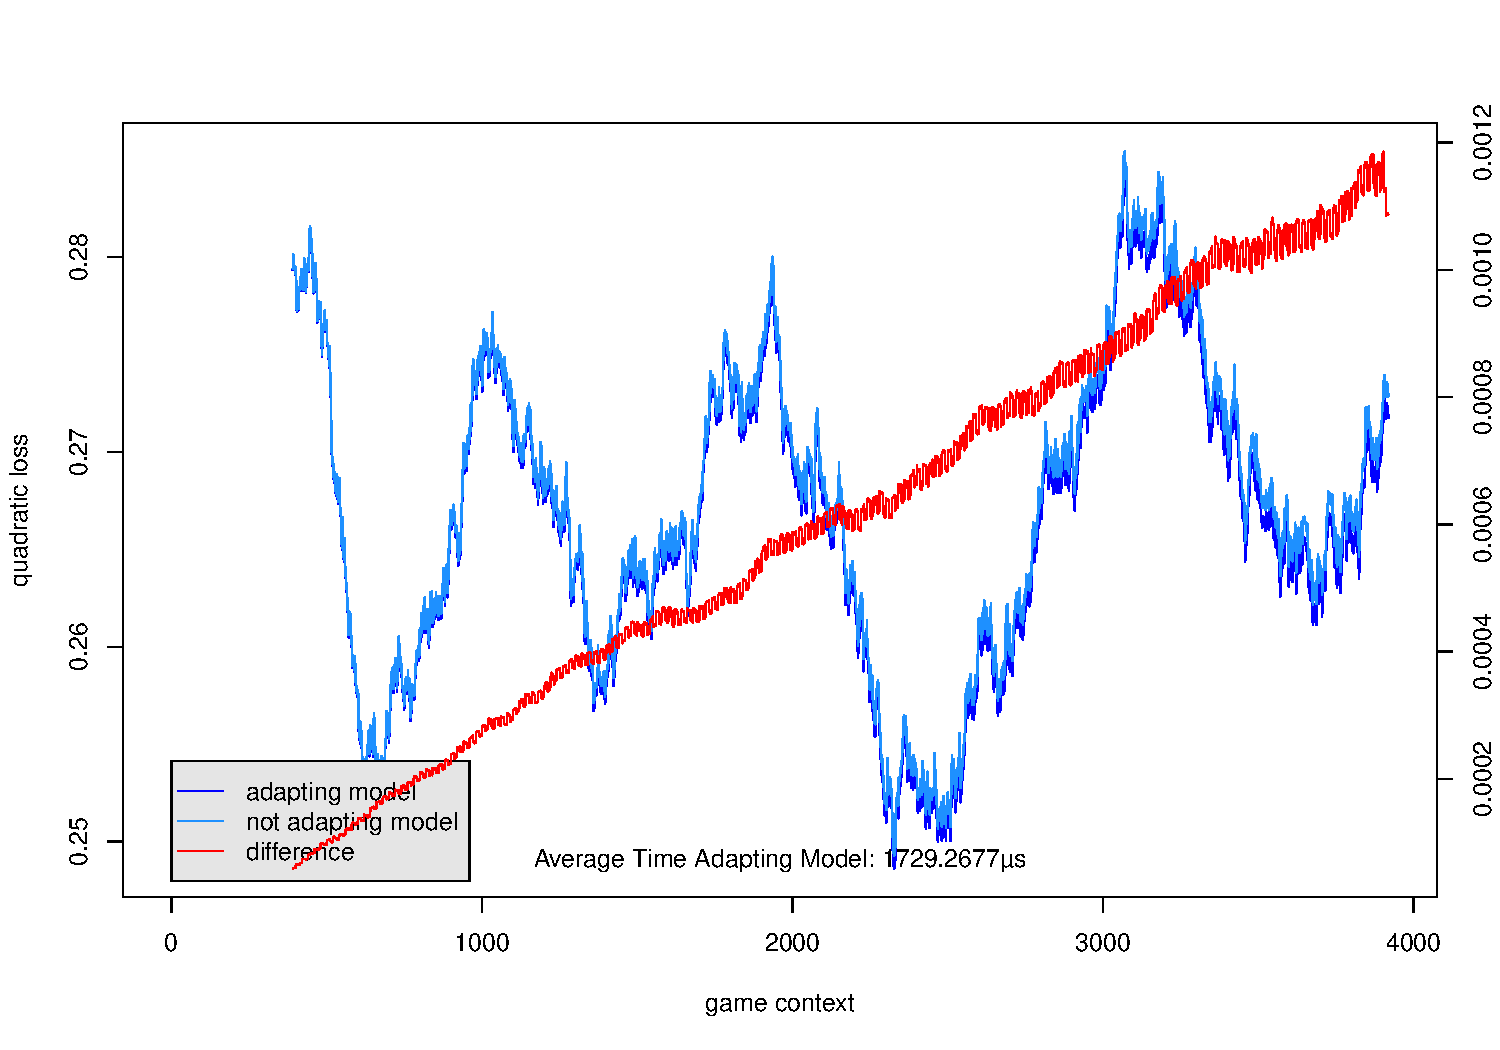
\includegraphics[scale=0.275]{section05-modelimpl/figures/HoeffdingTree-HyperboreanNL-Eqm-action-quadratic}
}
\subfigure[Model of HyperboreanNL-Eqm: Correctly Predicted]{
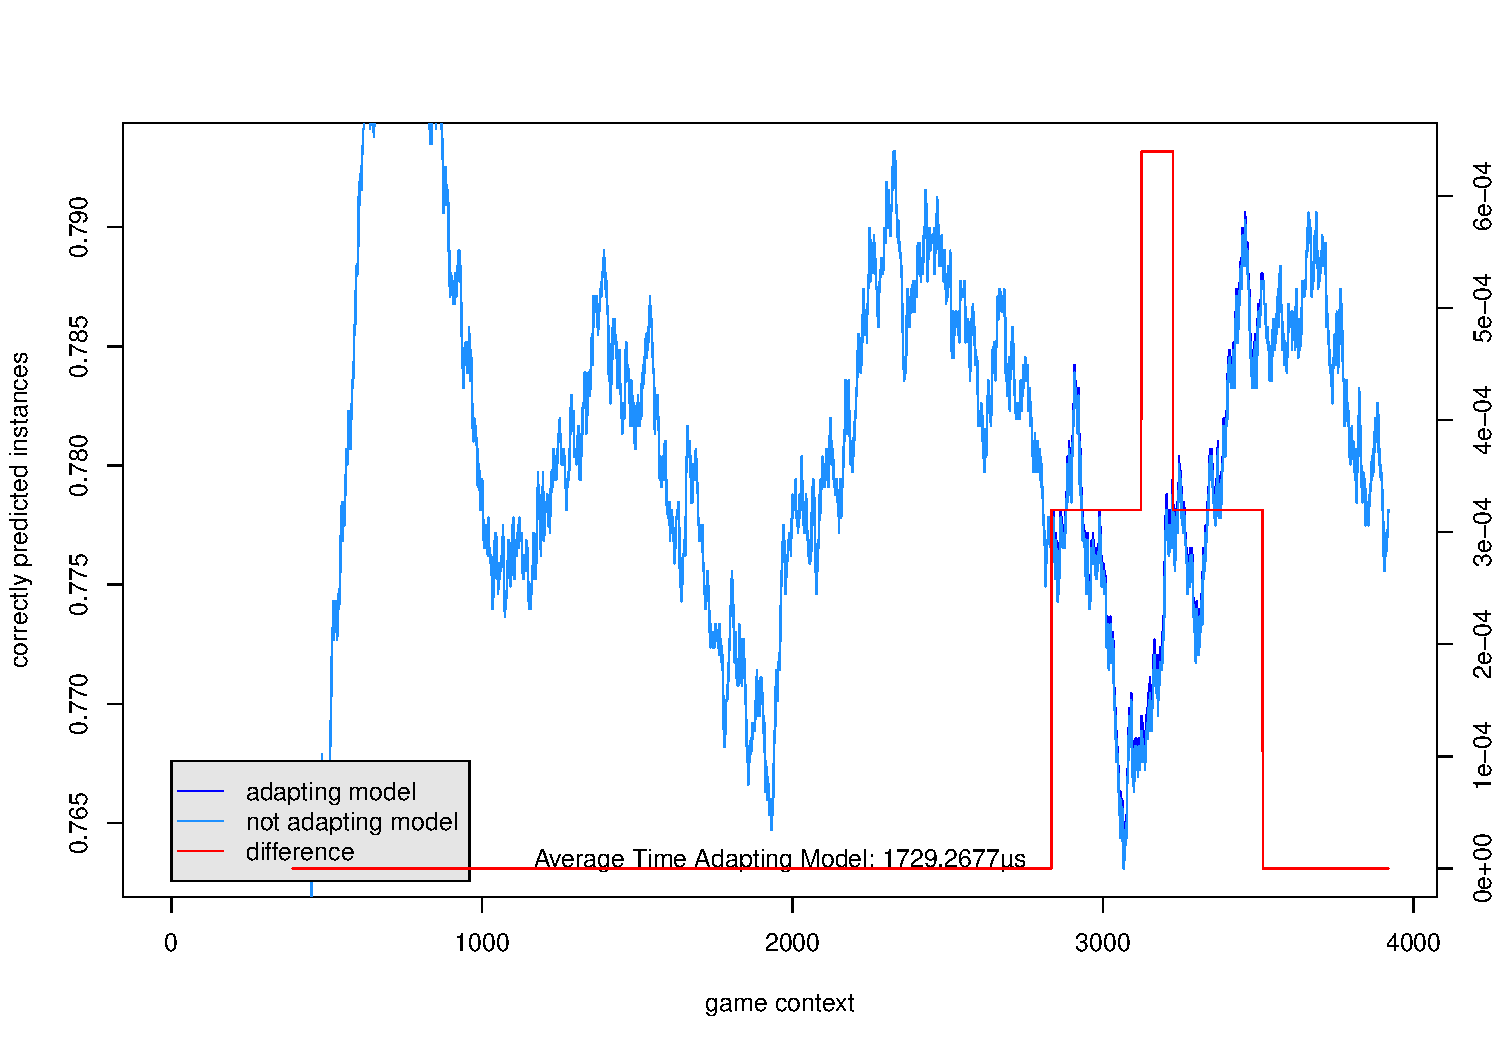
\includegraphics[scale=0.275]{section05-modelimpl/figures/HoeffdingTree-HyperboreanNL-Eqm-action-correctly}
}

\subfigure[Model of HyperboreanNL-BR: Quadratic Loss]{
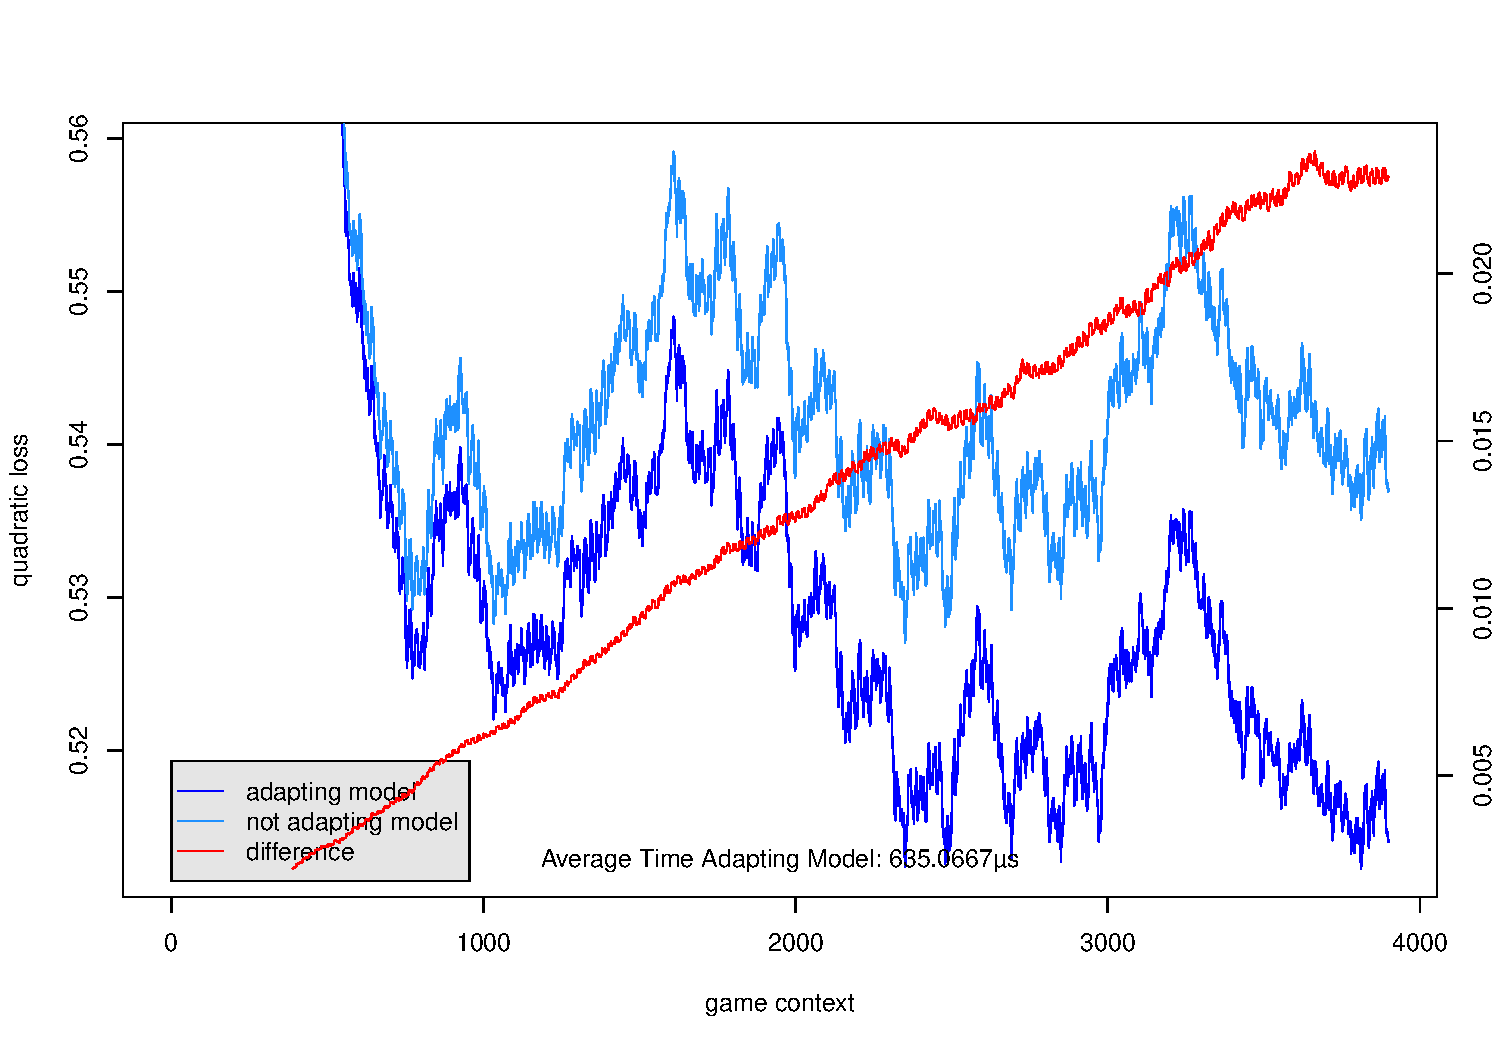
\includegraphics[scale=0.275]{section05-modelimpl/figures/HoeffdingTree-HyperboreanNL-BR-action-quadratic}
}
\subfigure[Model of HyperboreanNL-BR: Correctly Predicted]{
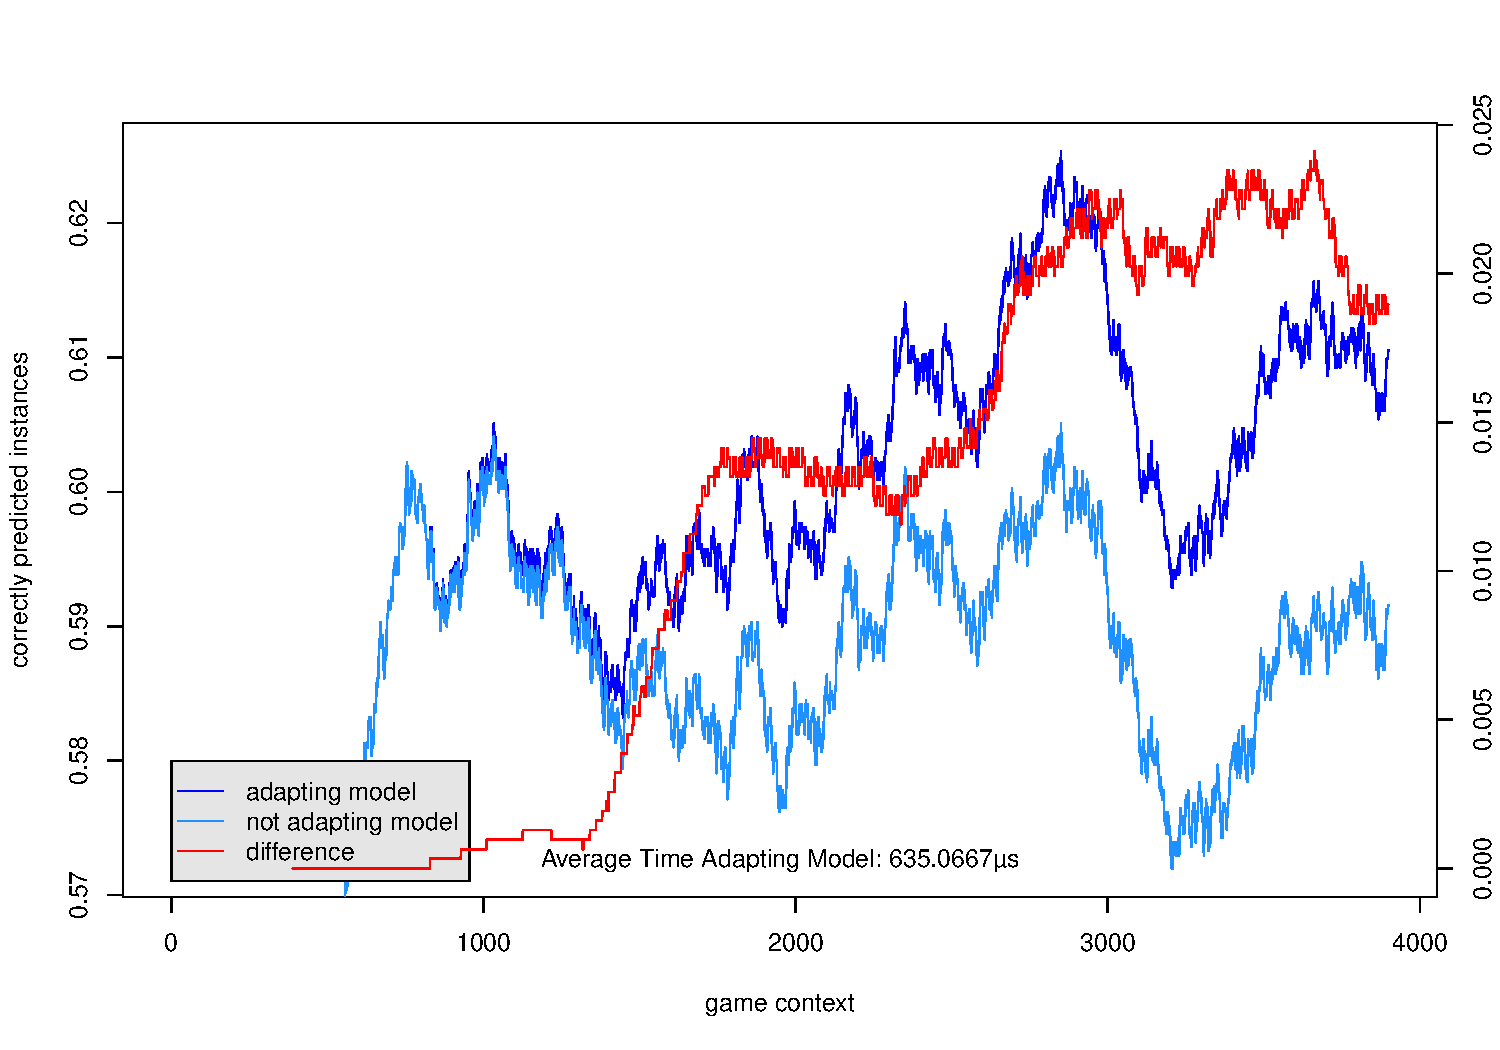
\includegraphics[scale=0.275]{section05-modelimpl/figures/HoeffdingTree-HyperboreanNL-BR-action-correctly}
}

\subfigure[Model of BluffBot4: Quadratic Loss]{
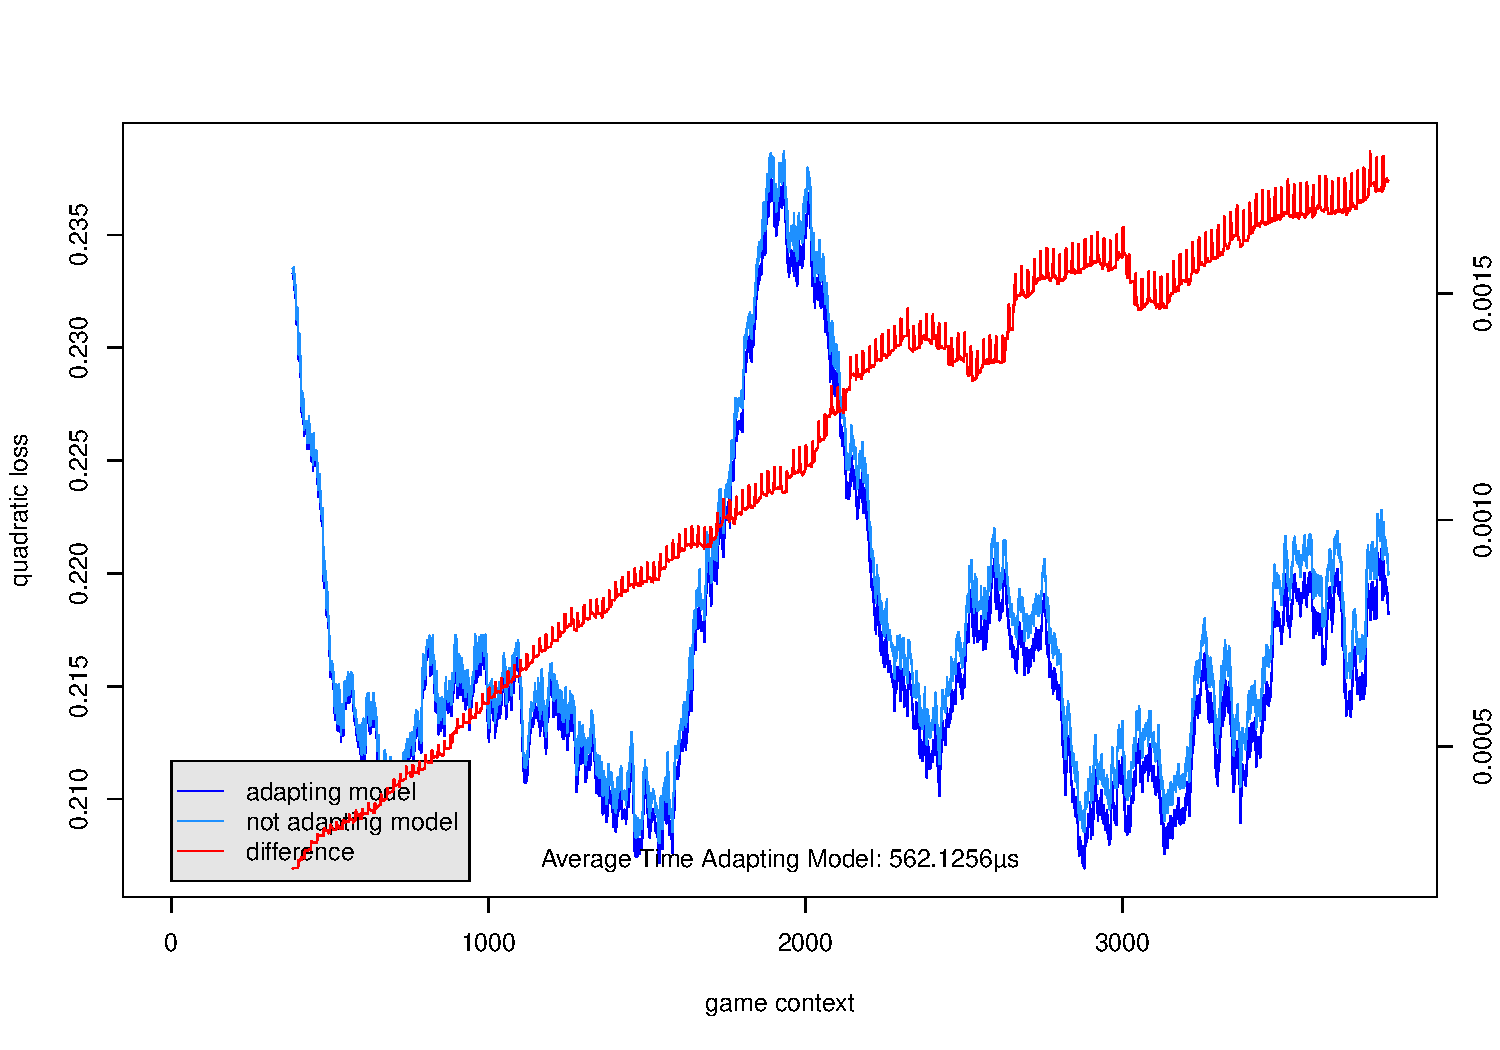
\includegraphics[scale=0.275]{section05-modelimpl/figures/HoeffdingTree-BluffBot4-action-quadratic}
}
\subfigure[Model of BluffBot4: Correctly Predicted]{
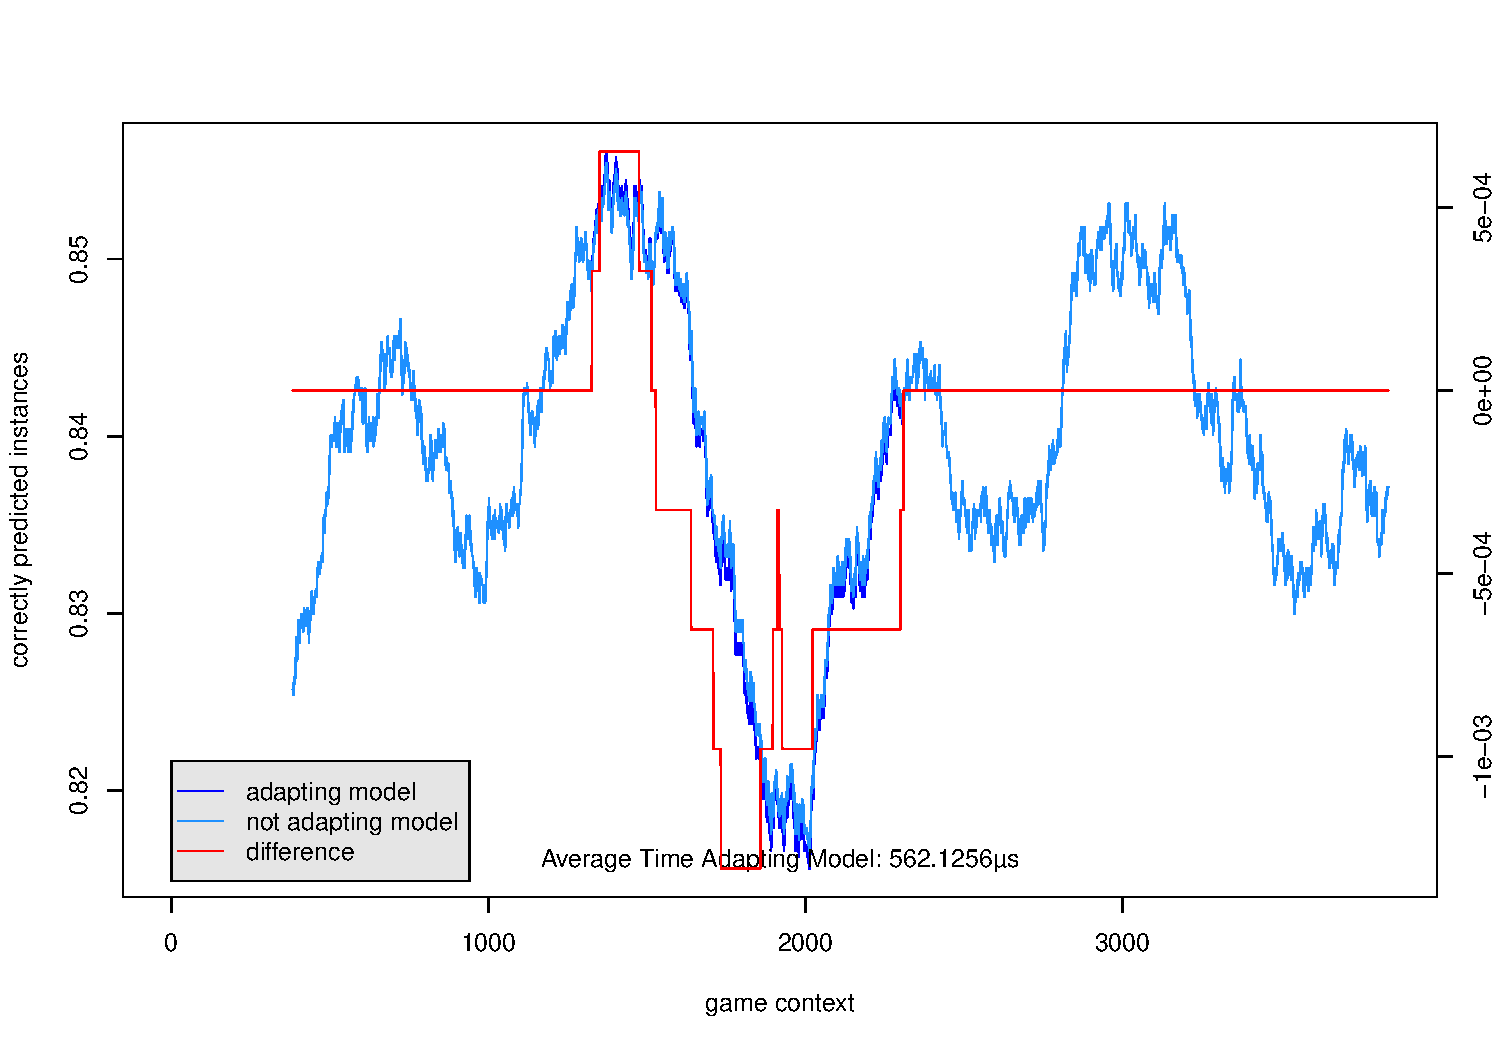
\includegraphics[scale=0.275]{section05-modelimpl/figures/HoeffdingTree-BluffBot4-action-correctly}
}


\caption{Action Prediction: Hoeffding Tree}
\label{fig:HoeffdingTree-action}
\end{figure}

\newpage
\subsection{Performance in Hand Prediction: Naive Bayes}
\begin{figure}[h!]
\centering

\subfigure[Model of HyperboreanNL-Eqm: Quadratic Loss]{
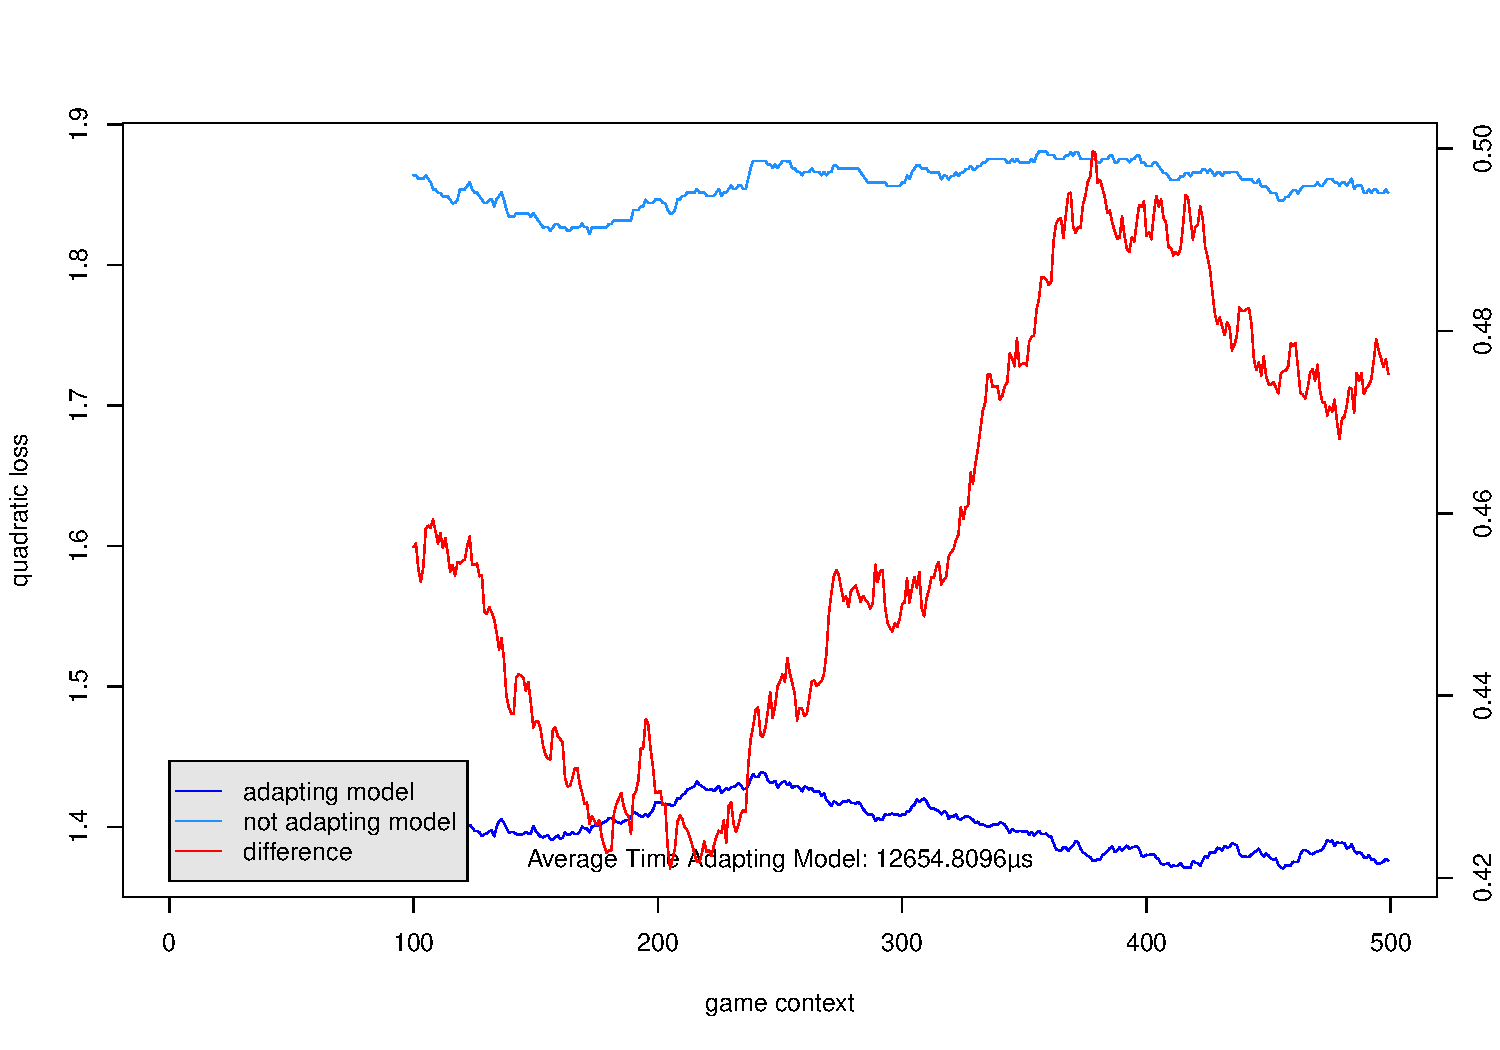
\includegraphics[scale=0.275]{section05-modelimpl/figures/MOANaiveBayes-HyperboreanNL-Eqm-hand-quadratic}
}
\subfigure[Model of HyperboreanNL-Eqm: Correctly Predicted]{
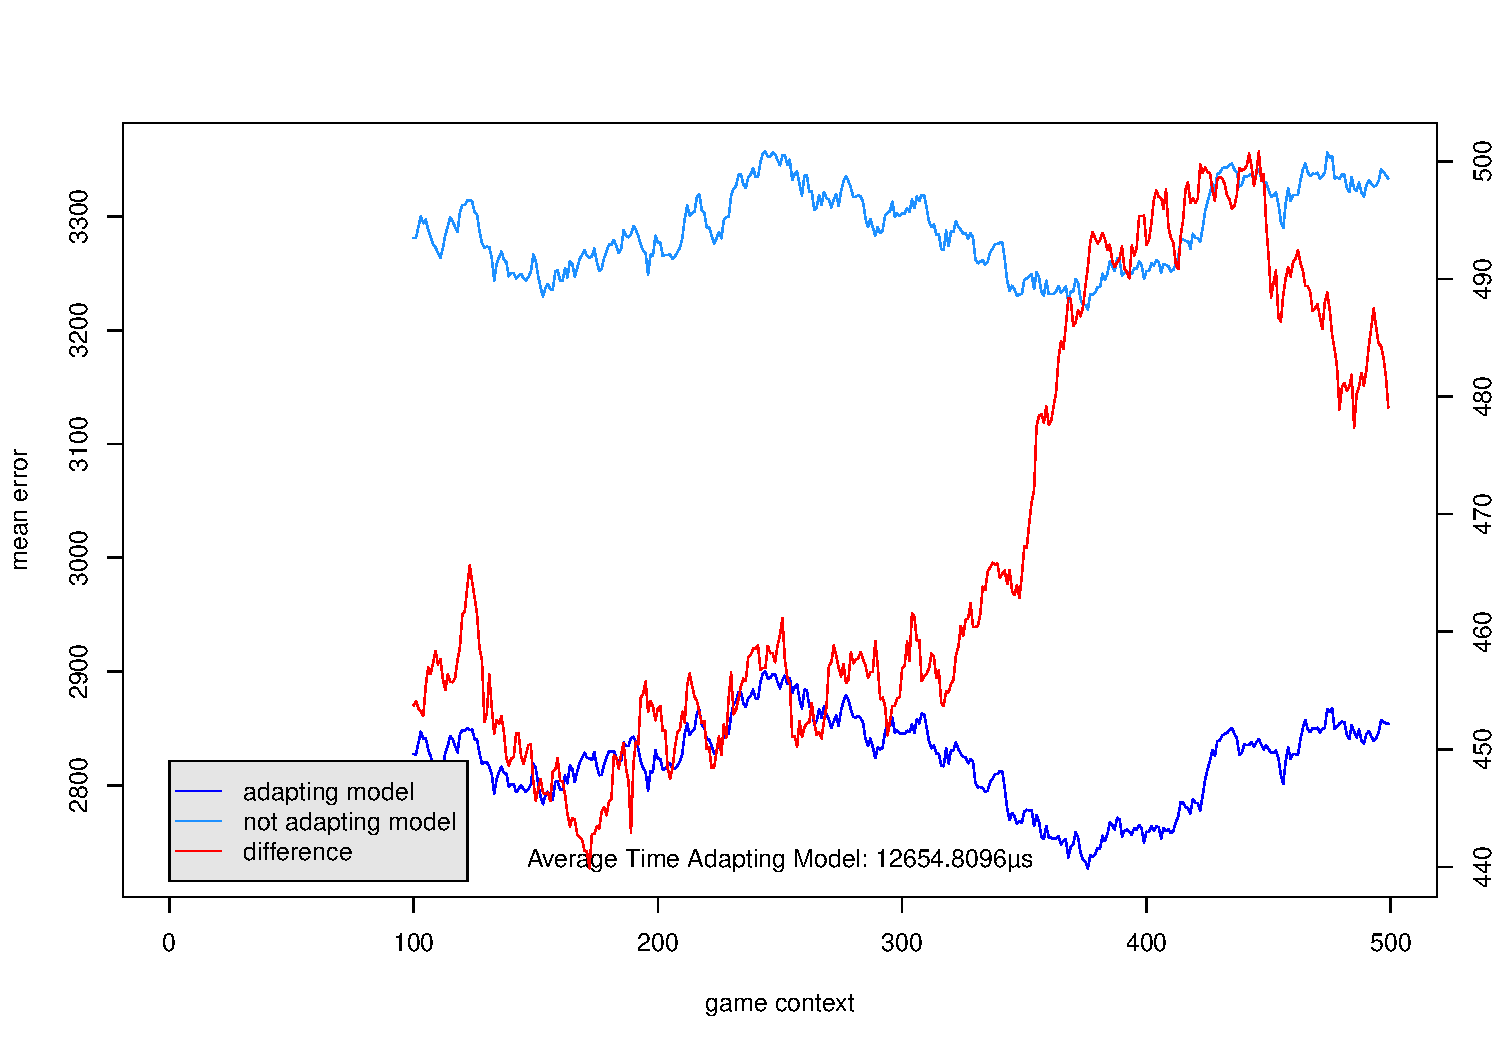
\includegraphics[scale=0.275]{section05-modelimpl/figures/MOANaiveBayes-HyperboreanNL-Eqm-hand-meansquared}
}

\subfigure[Model of HyperboreanNL-BR: Quadratic Loss]{
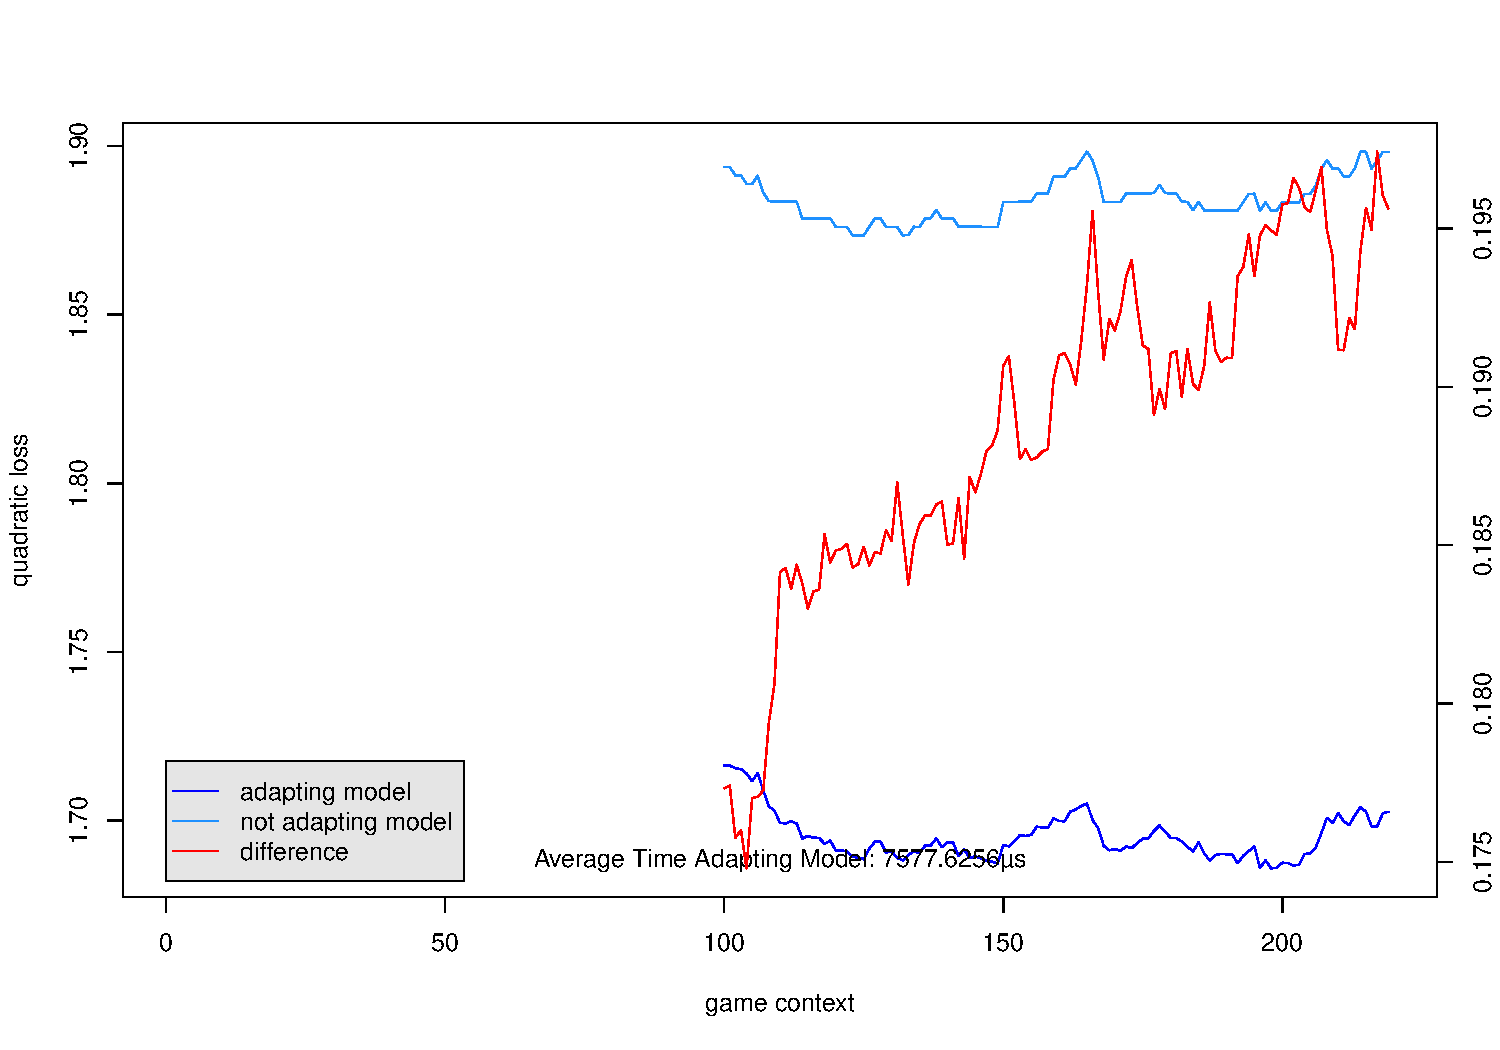
\includegraphics[scale=0.275]{section05-modelimpl/figures/MOANaiveBayes-HyperboreanNL-BR-hand-quadratic}
}
\subfigure[Model of HyperboreanNL-BR: Correctly Predicted]{
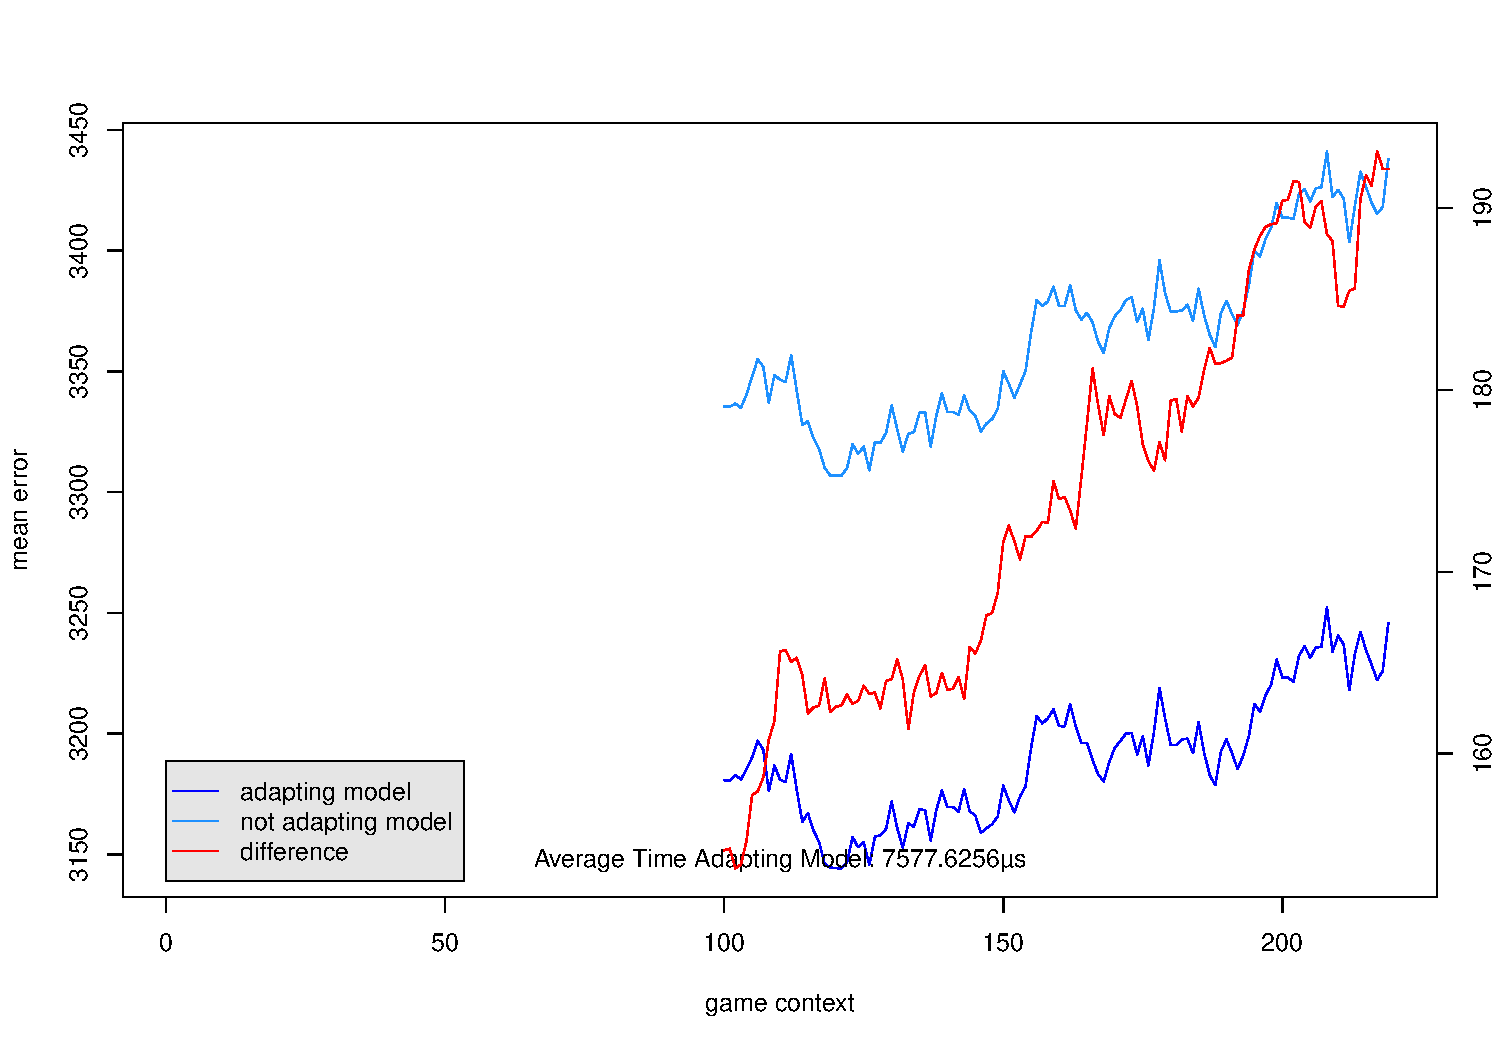
\includegraphics[scale=0.275]{section05-modelimpl/figures/MOANaiveBayes-HyperboreanNL-BR-hand-meansquared}
}

\subfigure[Model of BluffBot4: Quadratic Loss]{
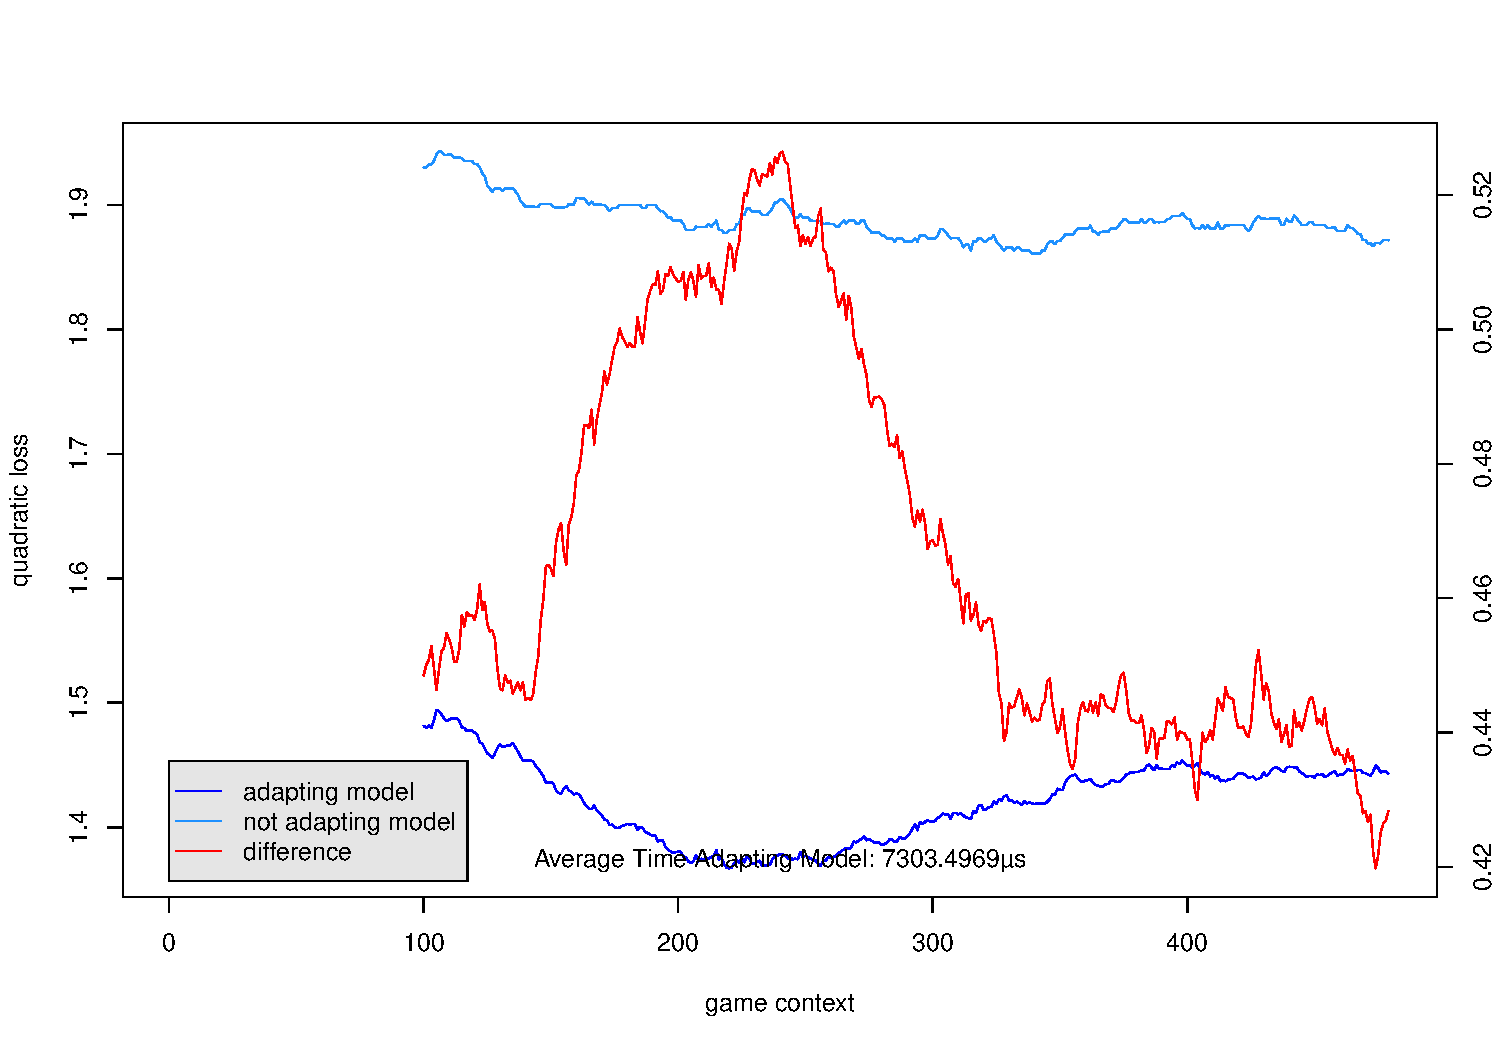
\includegraphics[scale=0.275]{section05-modelimpl/figures/MOANaiveBayes-BluffBot4-hand-quadratic}
}
\subfigure[Model of BluffBot4: Correctly Predicted]{
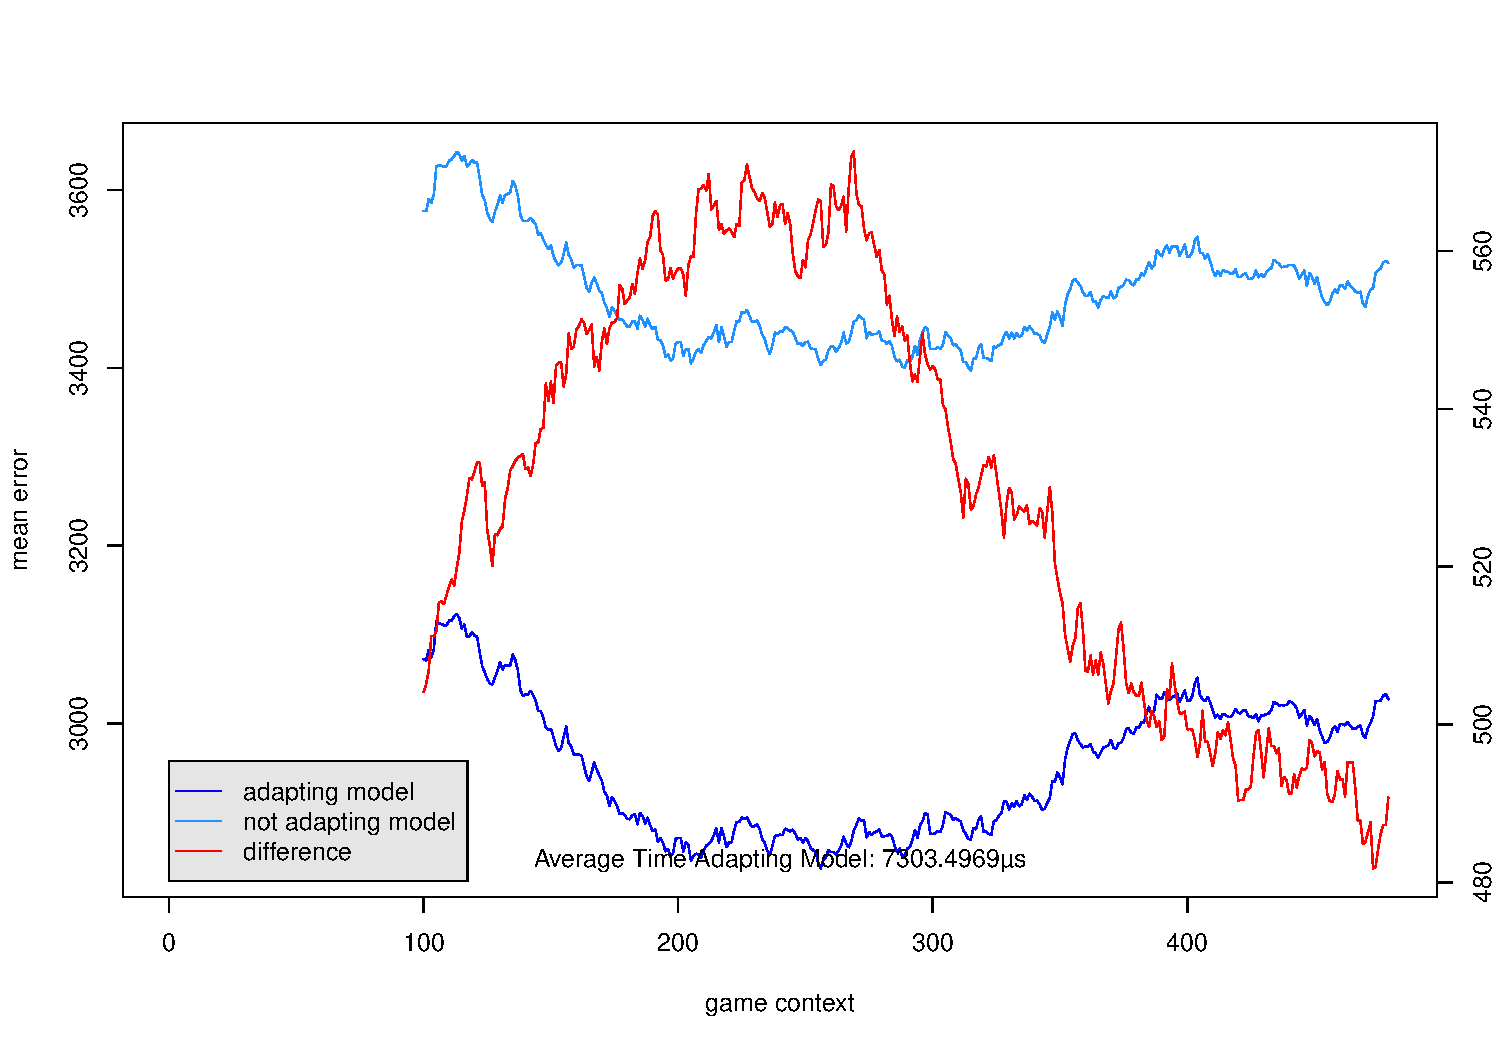
\includegraphics[scale=0.275]{section05-modelimpl/figures/MOANaiveBayes-BluffBot4-hand-meansquared}
}

\caption{Hand Prediction: Naive Bayes}
\label{fig:MOANaiveBayes-hand}
\end{figure}




\newpage
\subsection{Performance in Hand Prediction: Online Backpropagation}
\begin{figure}[h!]
\centering

\subfigure[Model of HyperboreanNL-Eqm: Quadratic Loss]{
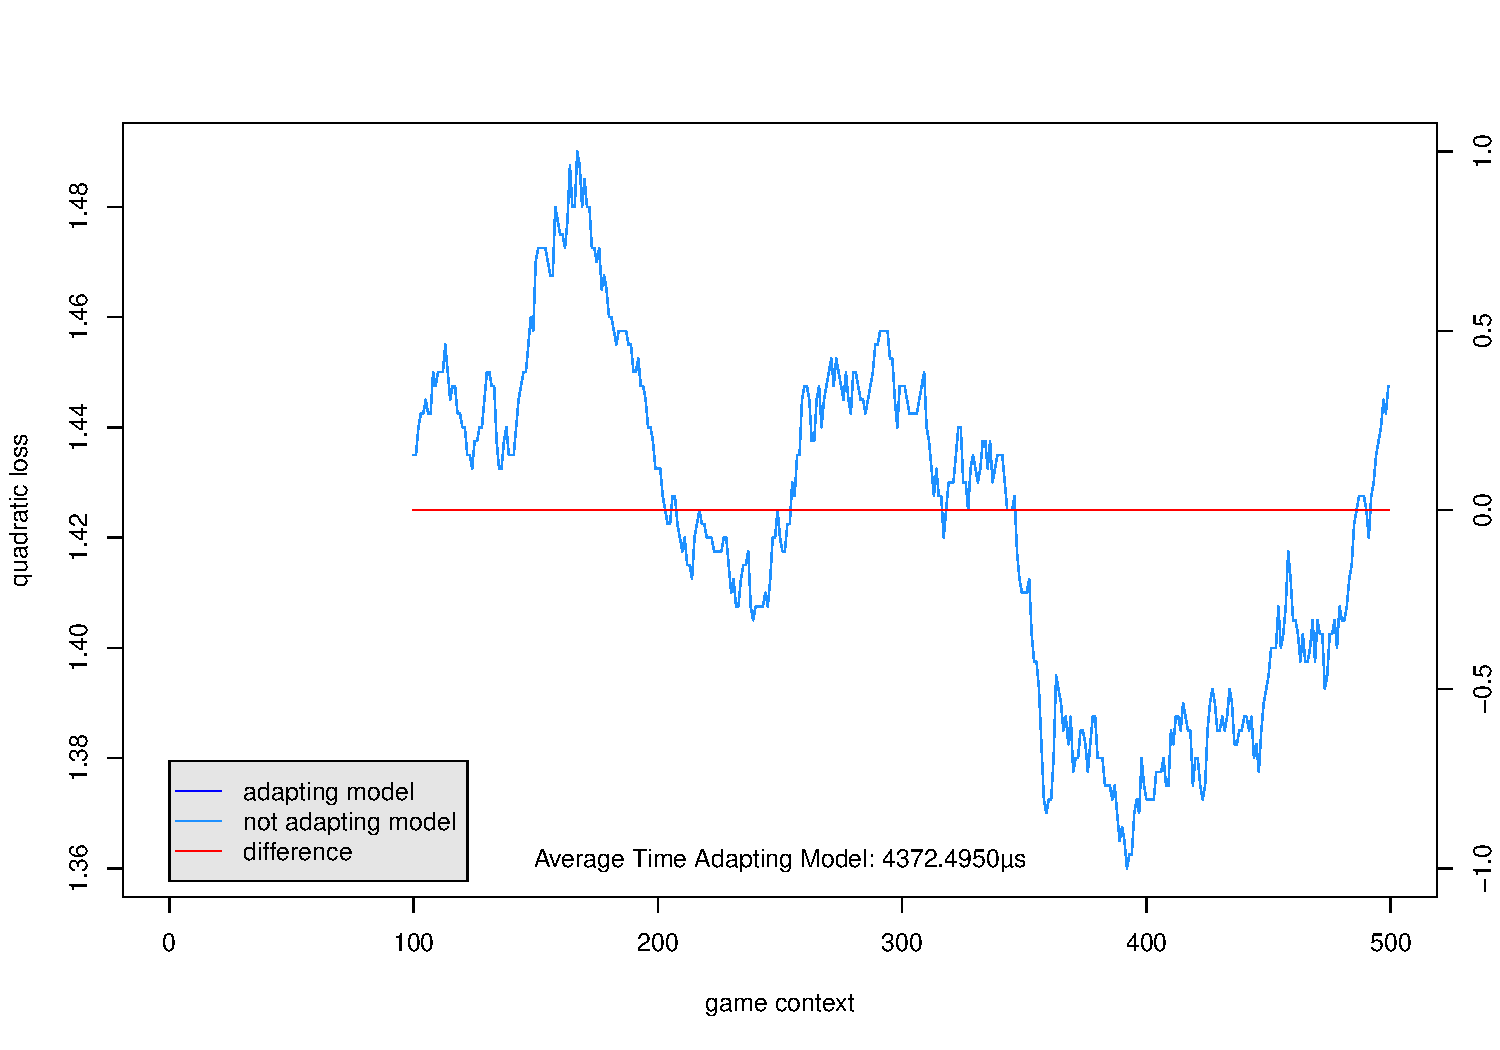
\includegraphics[scale=0.275]{section05-modelimpl/figures/OnlineBackpropagation-HyperboreanNL-Eqm-hand-quadratic}
}
\subfigure[Model of HyperboreanNL-Eqm: Mean Error]{
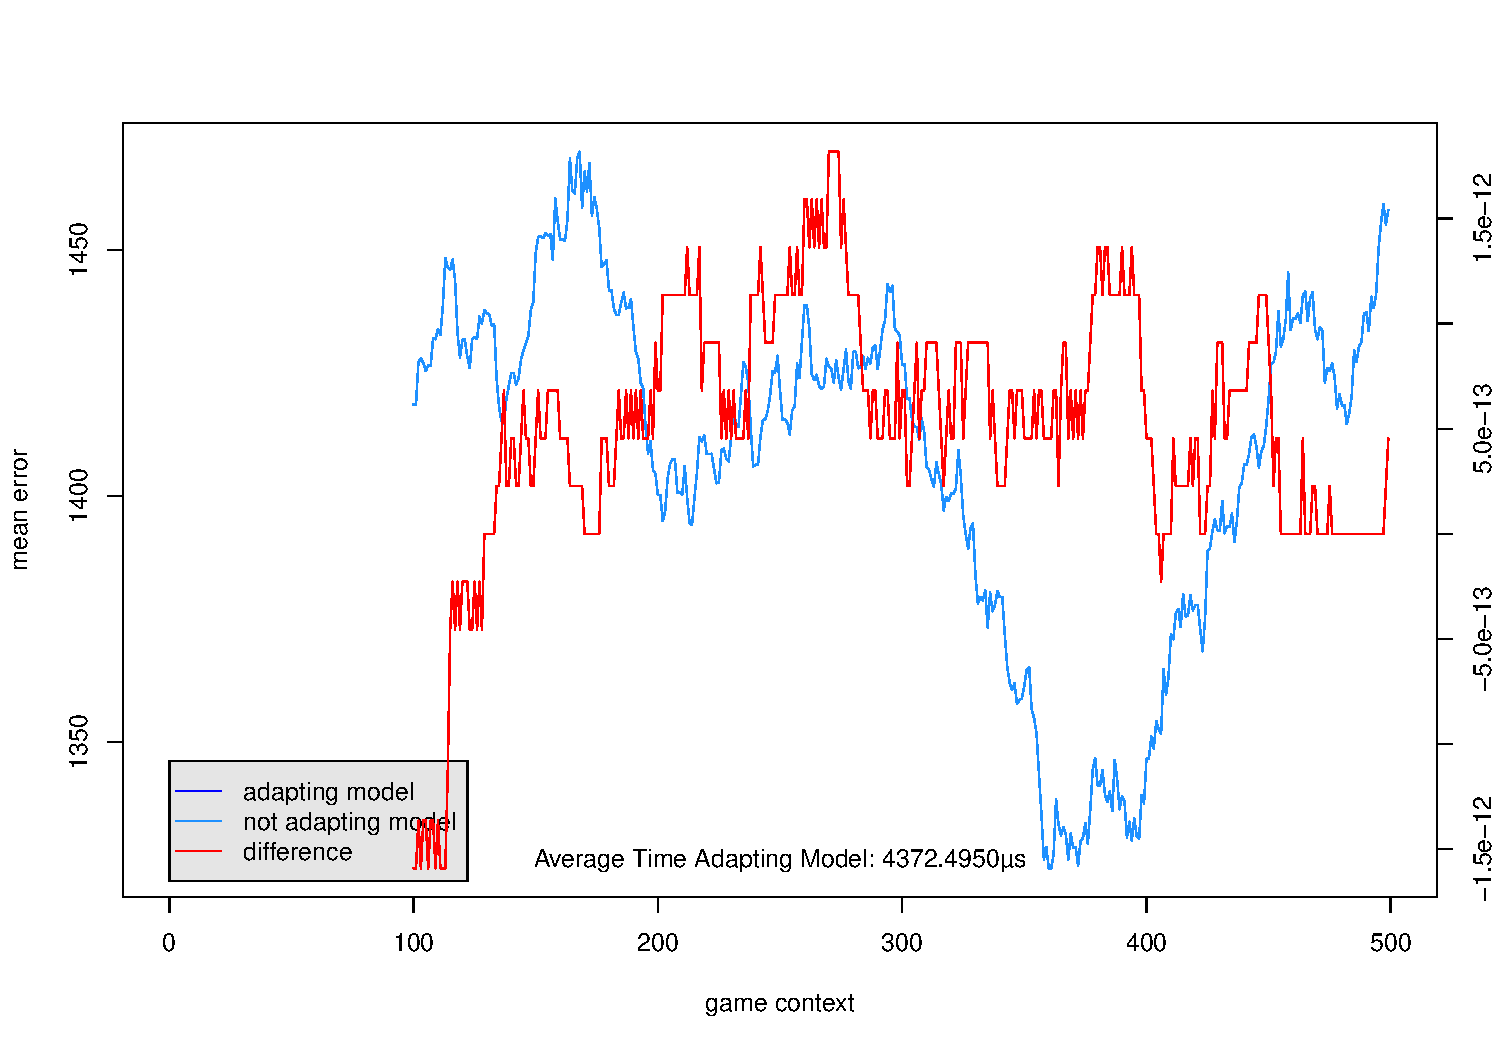
\includegraphics[scale=0.275]{section05-modelimpl/figures/OnlineBackpropagation-HyperboreanNL-Eqm-hand-meansquared}
}

\subfigure[Model of HyperboreanNL-BR: Quadratic Loss]{
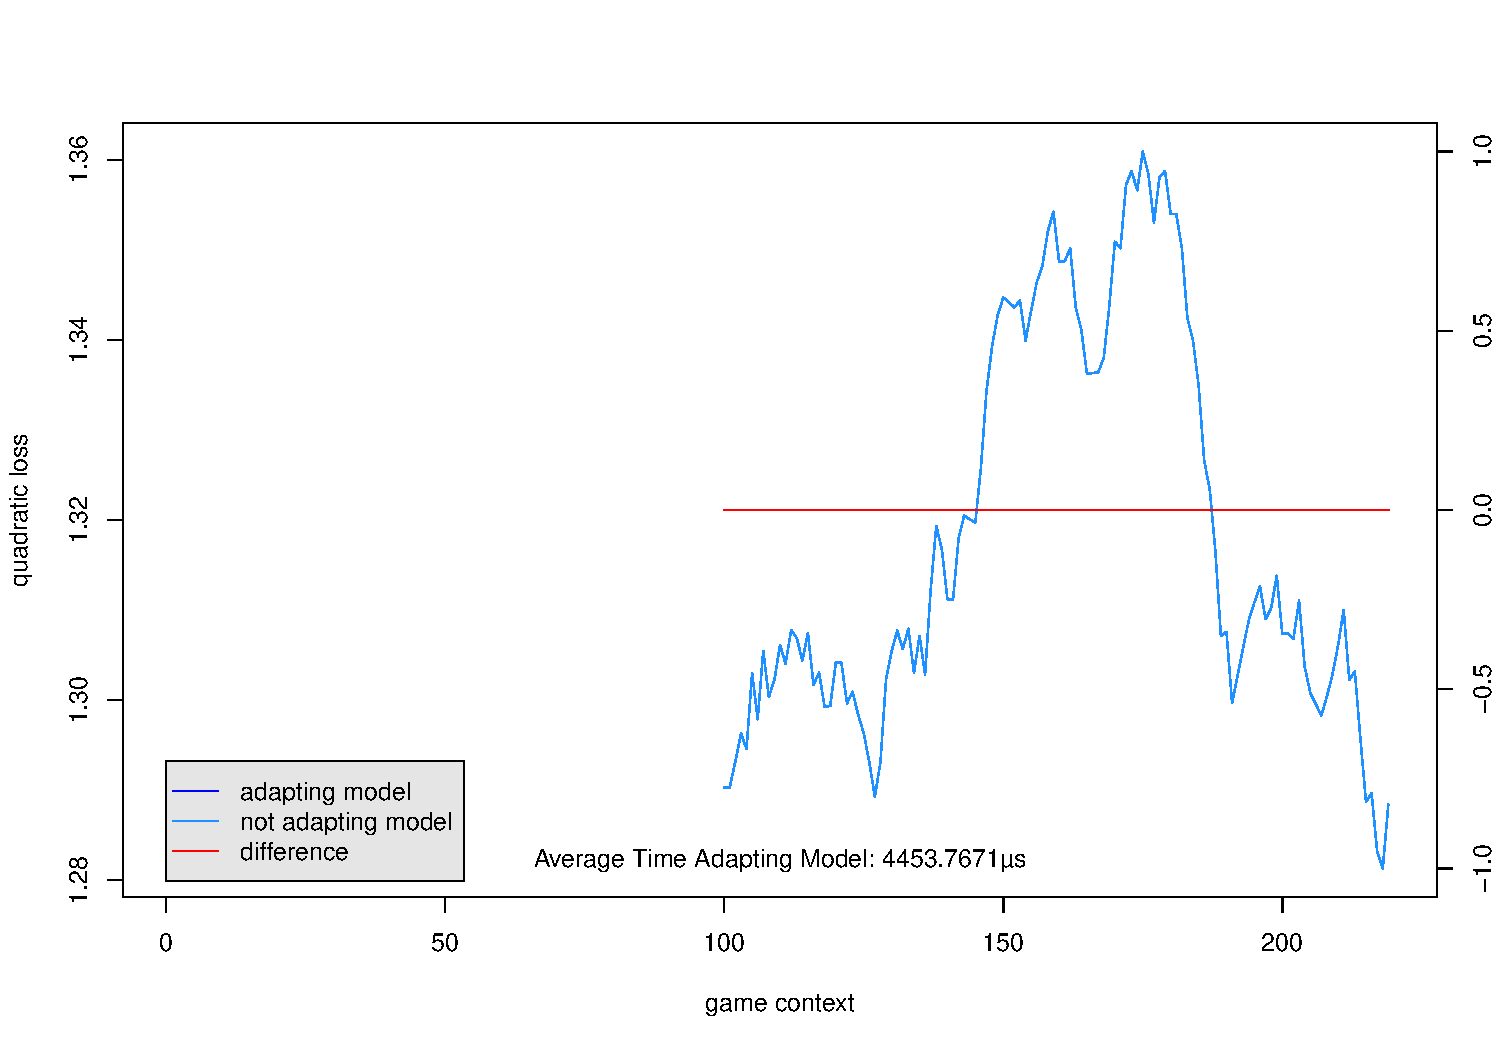
\includegraphics[scale=0.275]{section05-modelimpl/figures/OnlineBackpropagation-HyperboreanNL-BR-hand-quadratic}
}
\subfigure[Model of HyperboreanNL-BR: Mean Error]{
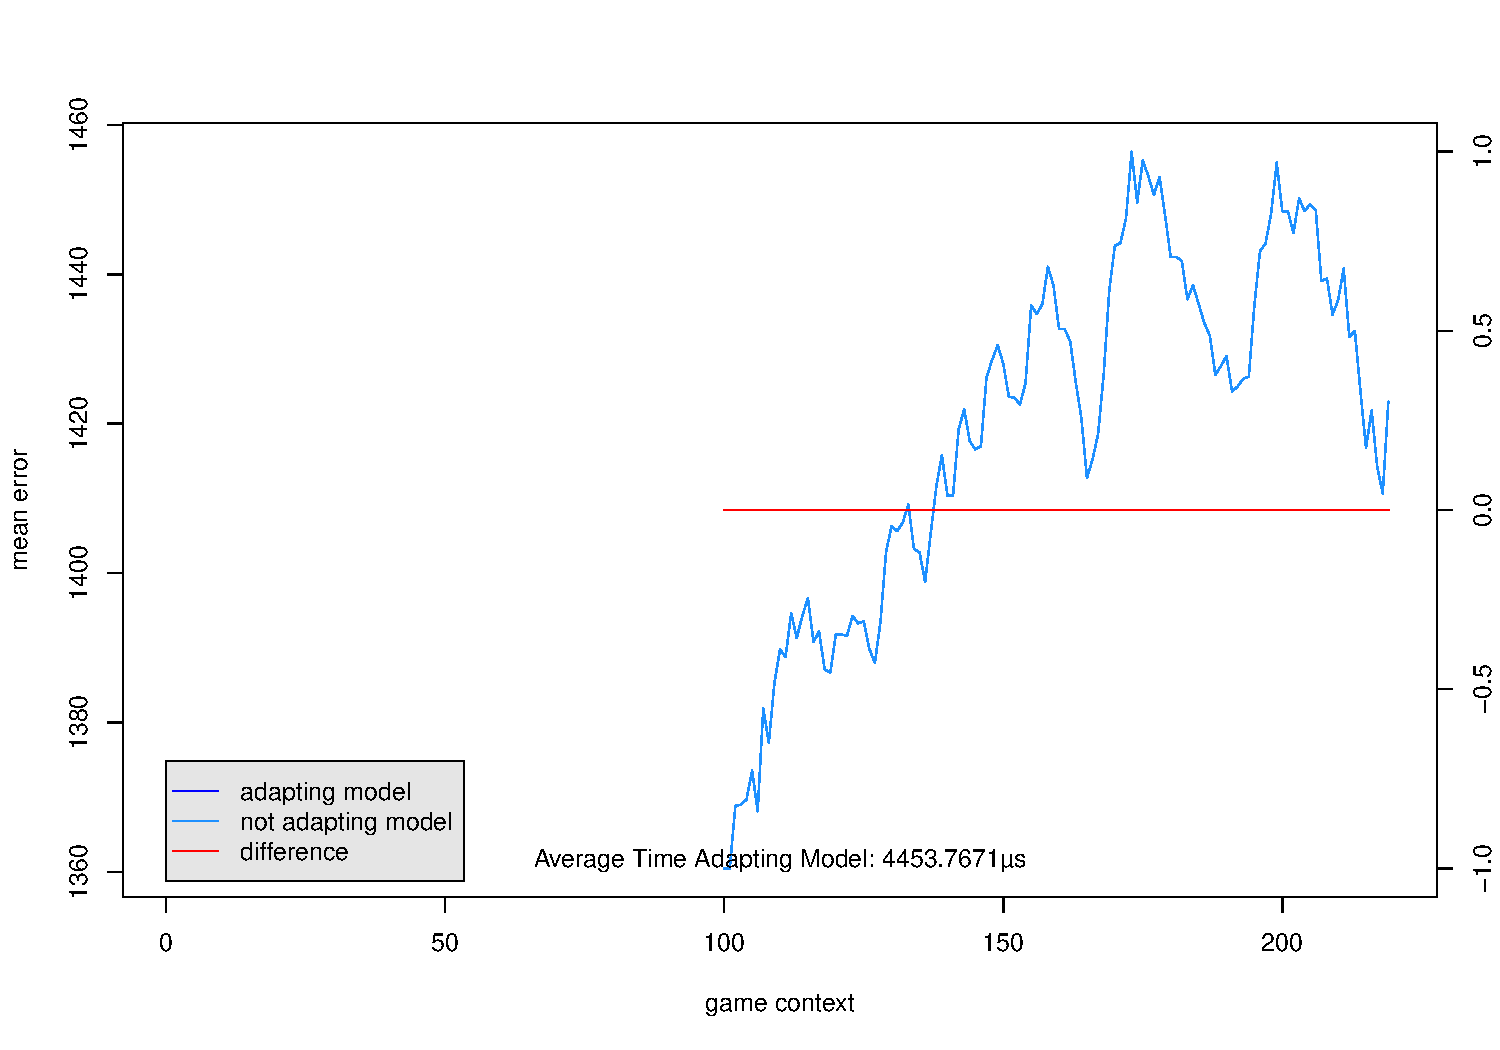
\includegraphics[scale=0.275]{section05-modelimpl/figures/OnlineBackpropagation-HyperboreanNL-BR-hand-meansquared}
}

\subfigure[Model of BluffBot4: Quadratic Loss]{
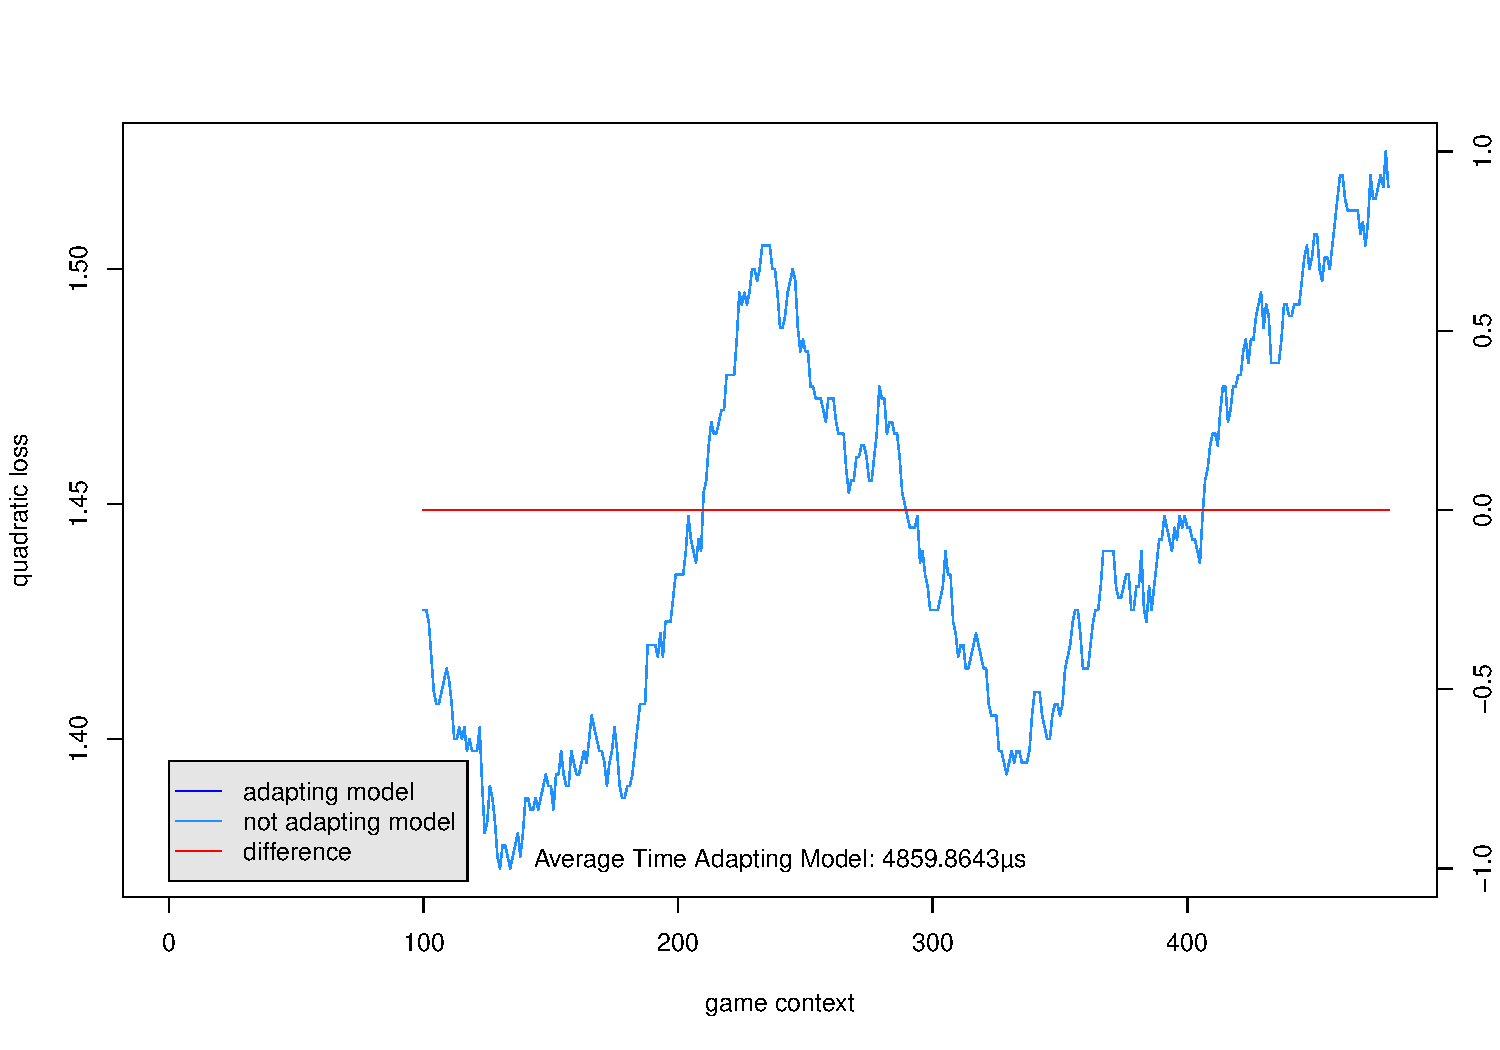
\includegraphics[scale=0.275]{section05-modelimpl/figures/OnlineBackpropagation-BluffBot4-hand-quadratic}
}
\subfigure[Model of BluffBot4: Mean Error]{
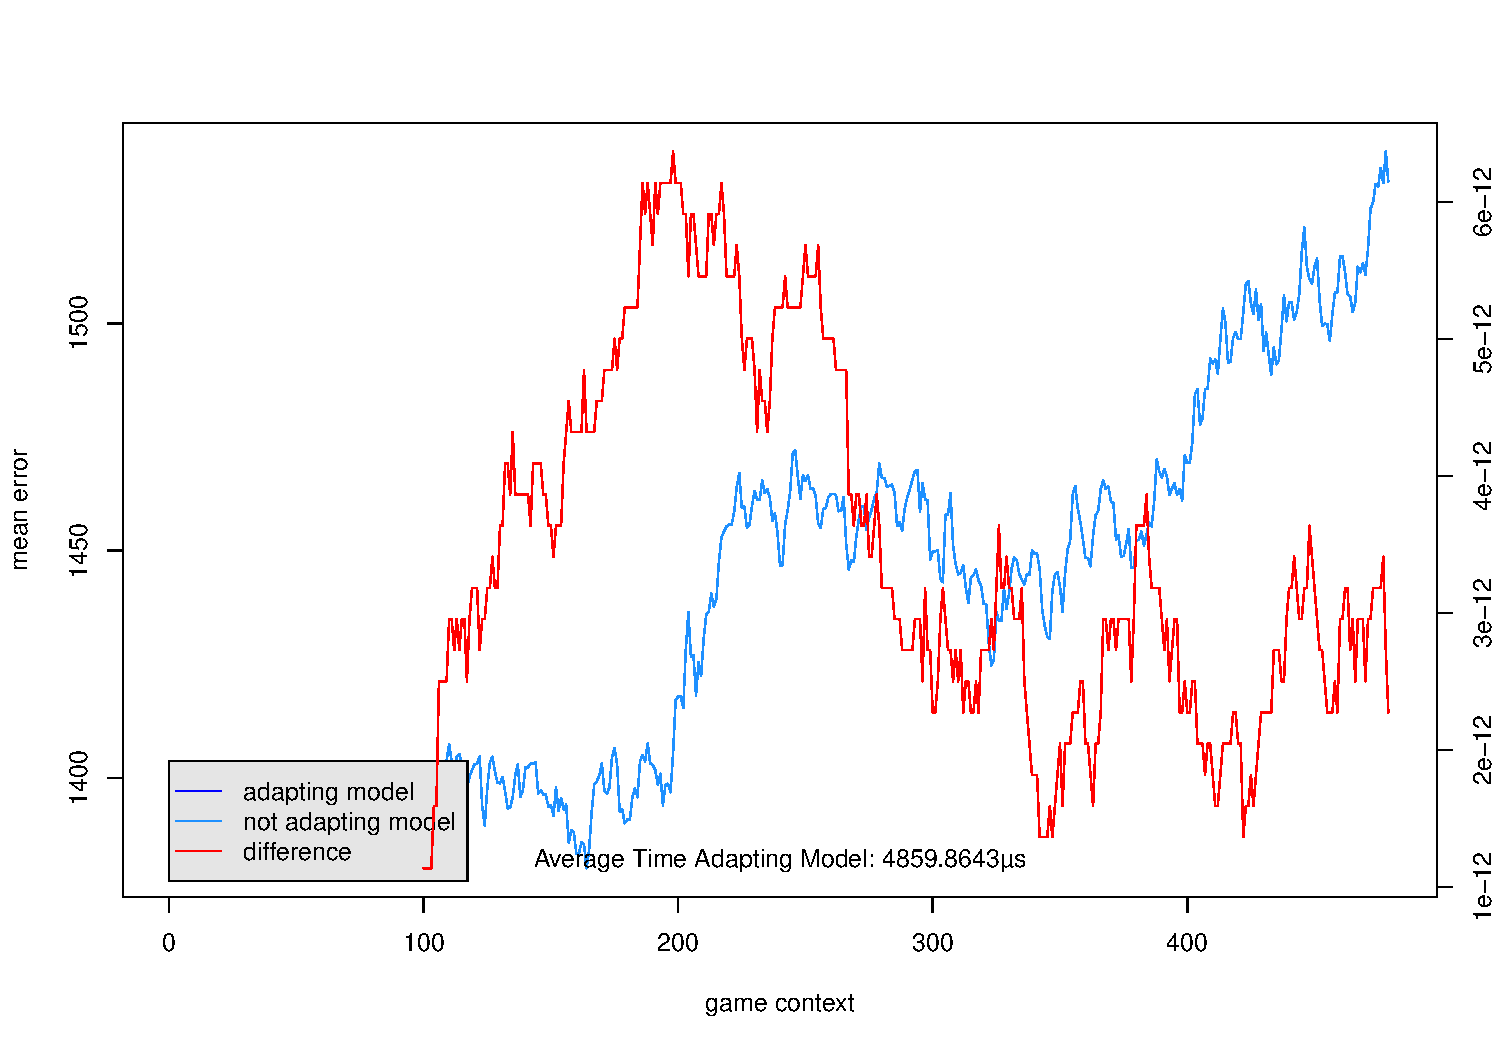
\includegraphics[scale=0.275]{section05-modelimpl/figures/OnlineBackpropagation-BluffBot4-hand-meansquared}
}

\caption{Hand Prediction: Online Backpropagation}
\label{fig:OnlineBackpropagation-hand}
\end{figure}


\newpage
\subsection{Performance in Hand Prediction: Hoeffding Tree}
\begin{figure}[h!]
\centering

\subfigure[Model of HyperboreanNL-Eqm: Quadratic Loss]{
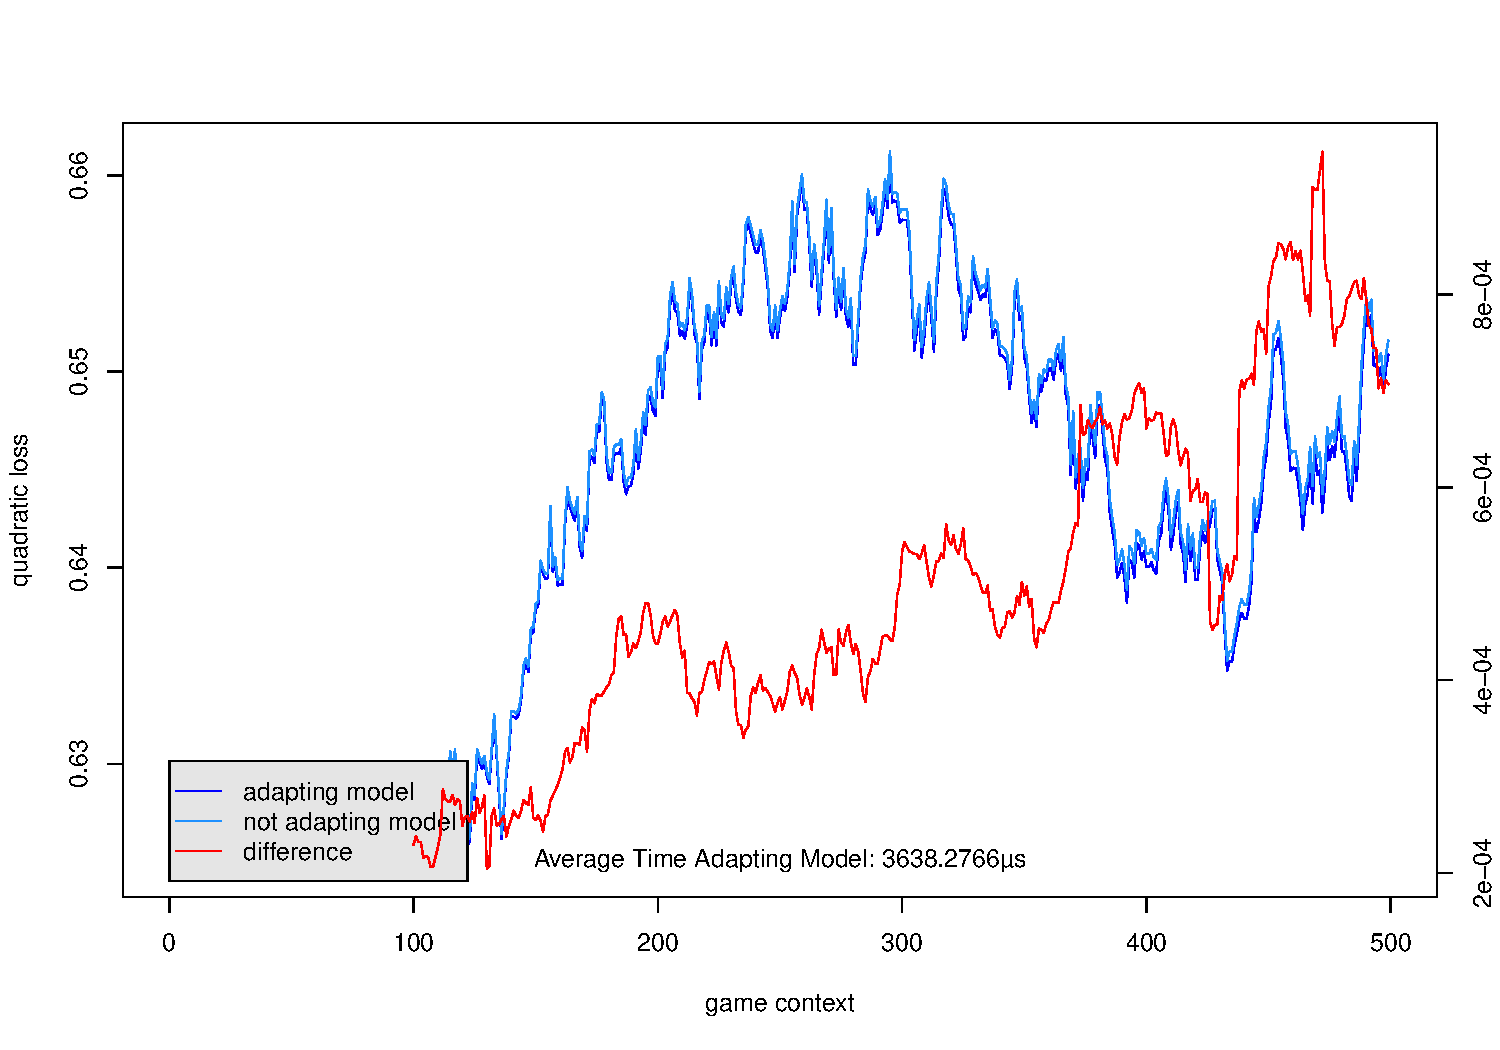
\includegraphics[scale=0.275]{section05-modelimpl/figures/HoeffdingTree-HyperboreanNL-Eqm-hand-quadratic}
}
\subfigure[Model of HyperboreanNL-Eqm: Mean Error]{
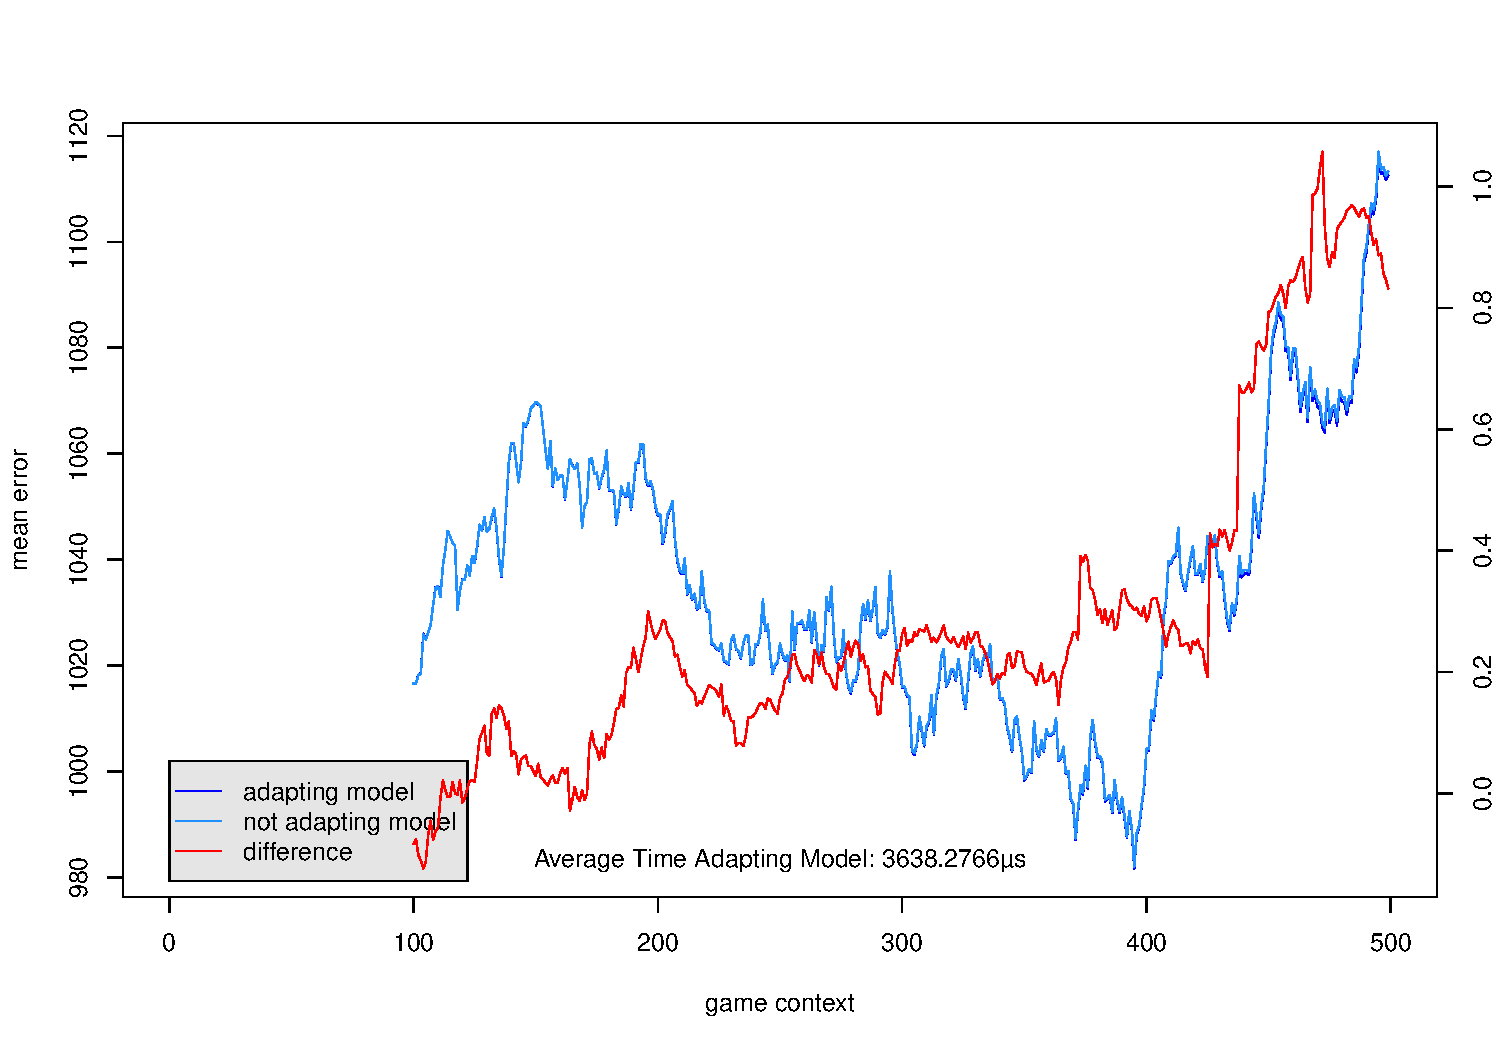
\includegraphics[scale=0.275]{section05-modelimpl/figures/HoeffdingTree-HyperboreanNL-Eqm-hand-meansquared}
}

\subfigure[Model of HyperboreanNL-BR: Quadratic Loss]{
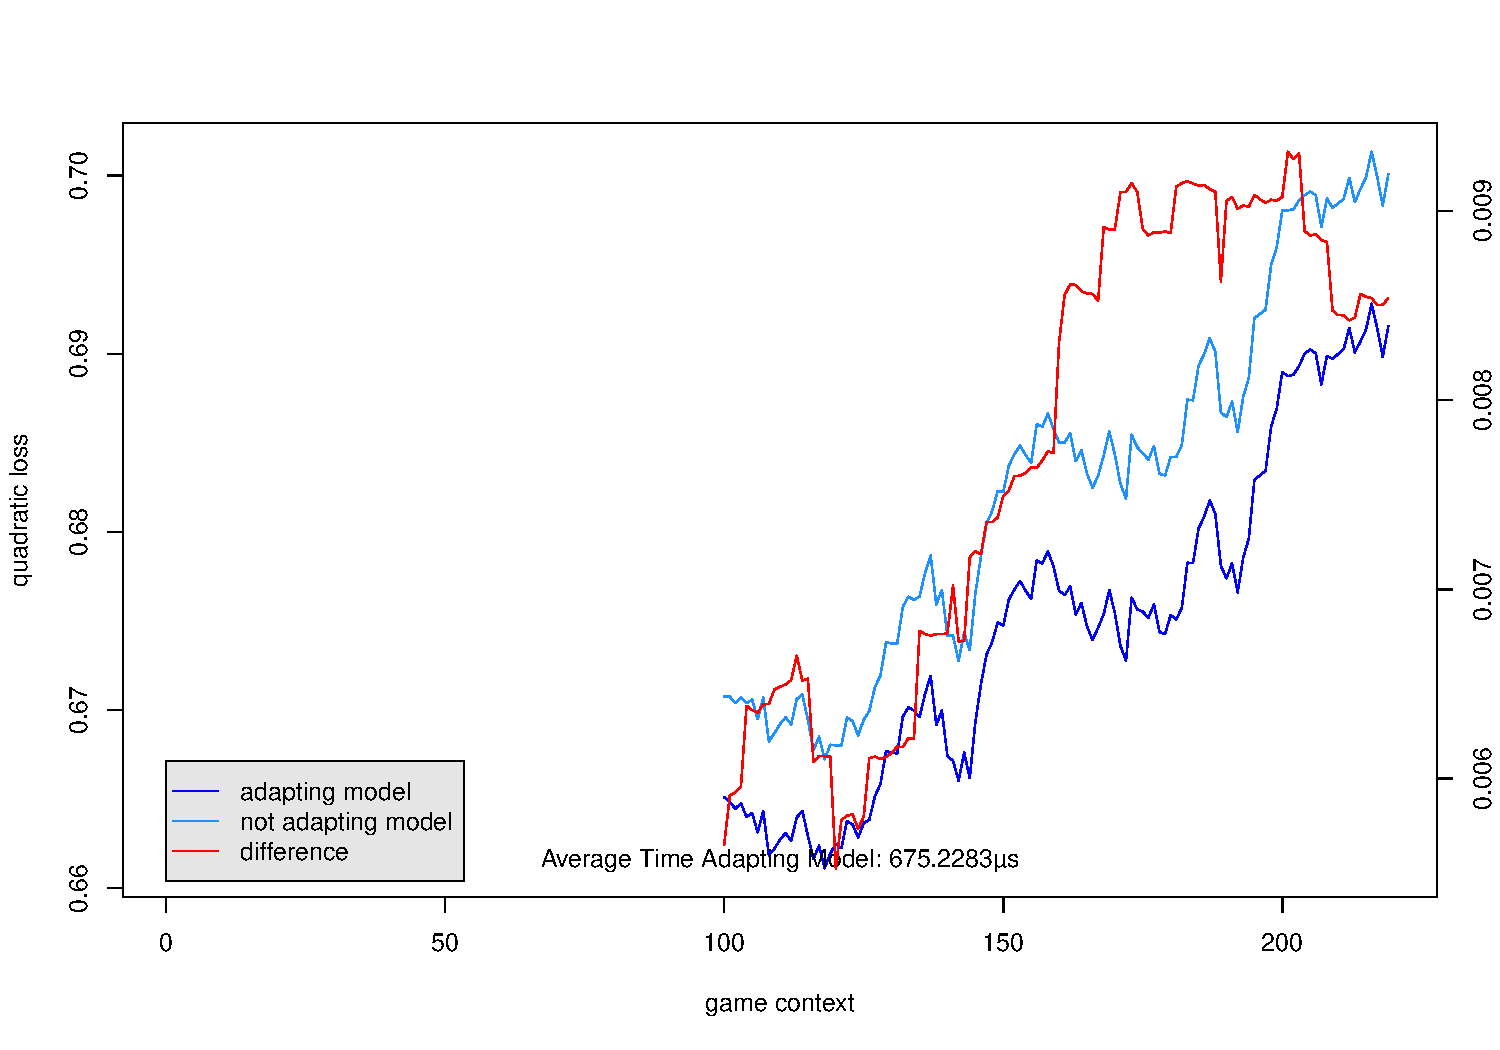
\includegraphics[scale=0.275]{section05-modelimpl/figures/HoeffdingTree-HyperboreanNL-BR-hand-quadratic}
}
\subfigure[Model of HyperboreanNL-BR: Mean Error]{
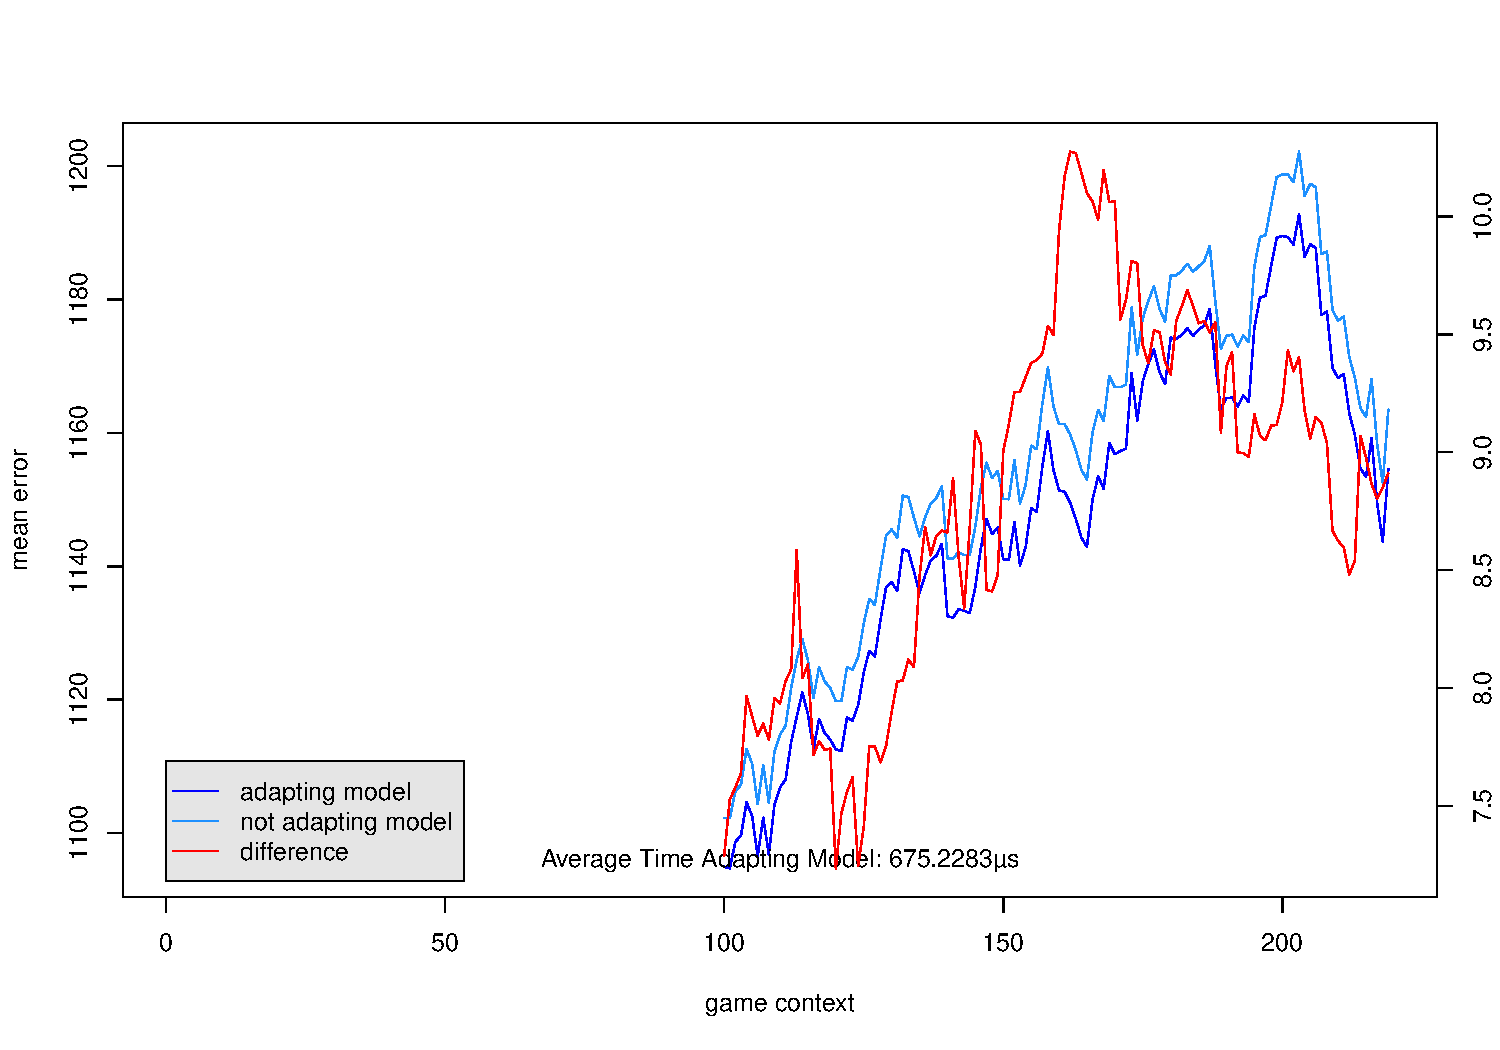
\includegraphics[scale=0.275]{section05-modelimpl/figures/HoeffdingTree-HyperboreanNL-BR-hand-meansquared}
}

\subfigure[Model of BluffBot4: Quadratic Loss]{
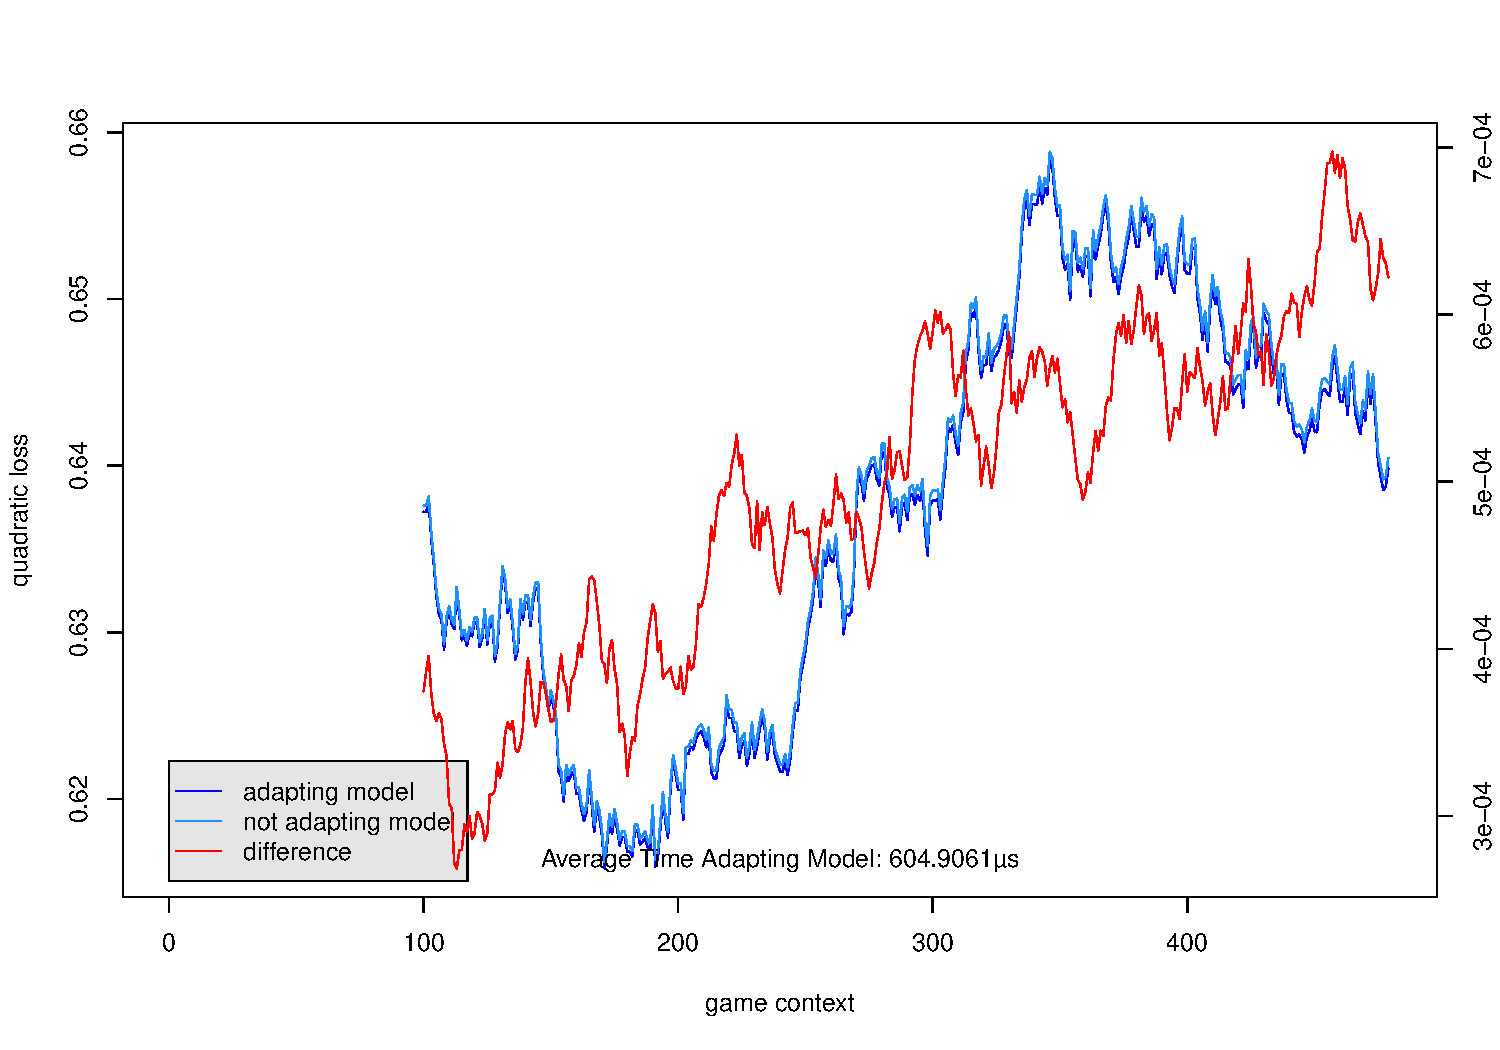
\includegraphics[scale=0.275]{section05-modelimpl/figures/HoeffdingTree-BluffBot4-hand-quadratic}
}
\subfigure[Model of BluffBot4: Mean Error]{
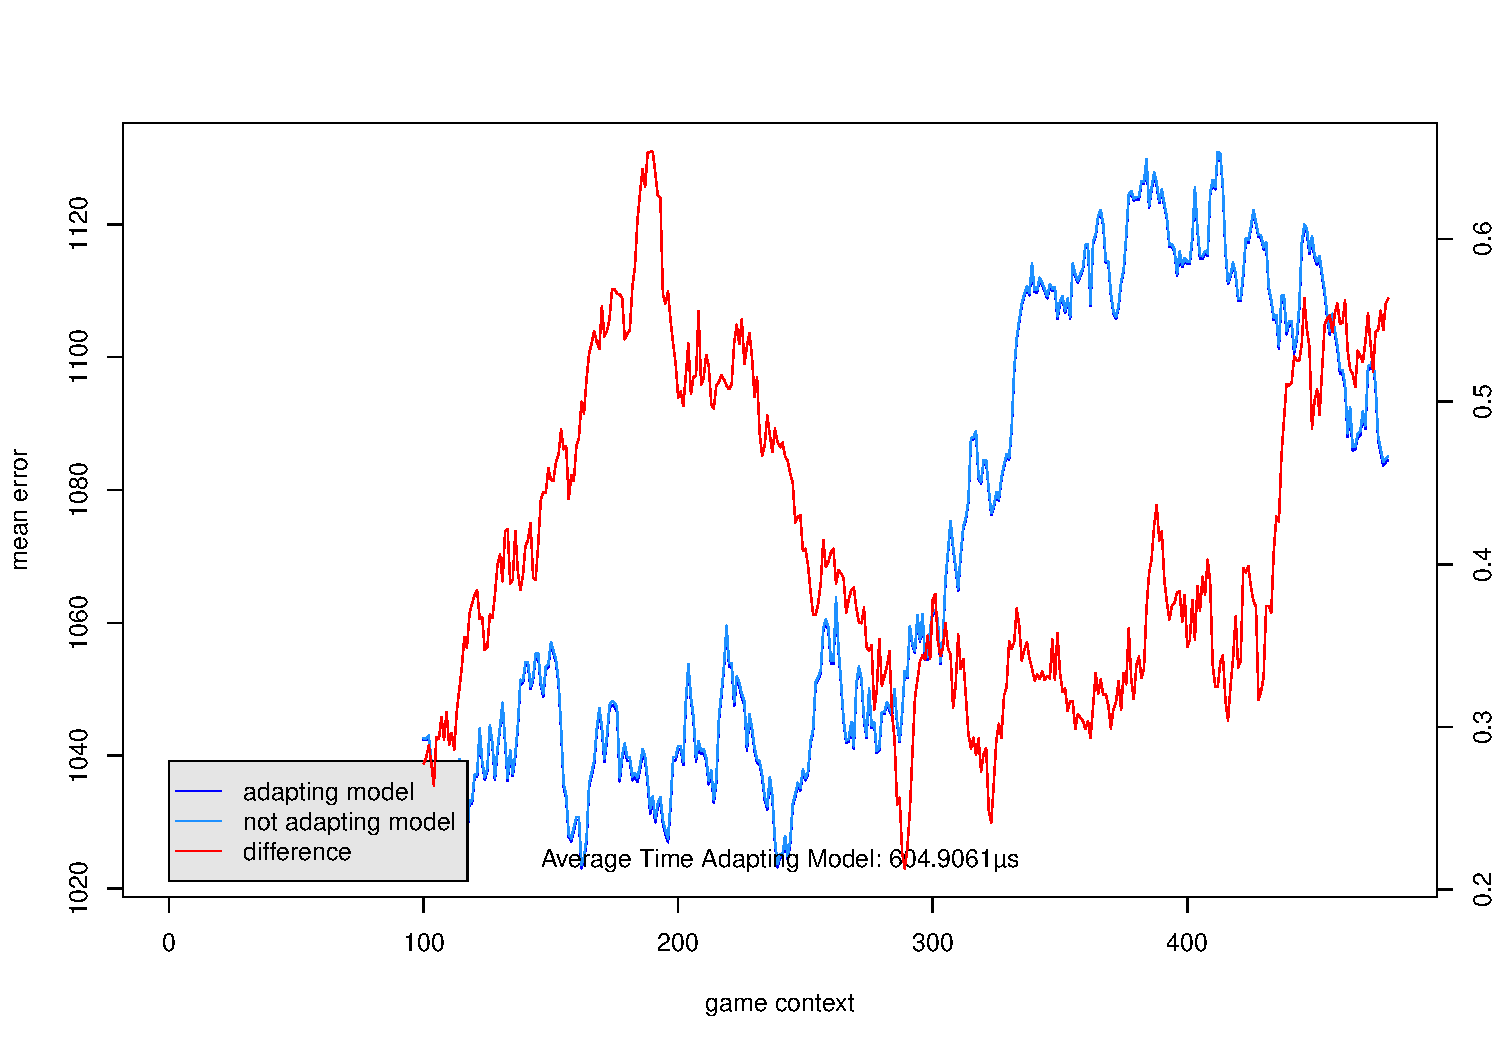
\includegraphics[scale=0.275]{section05-modelimpl/figures/HoeffdingTree-BluffBot4-hand-meansquared}
}


\caption{Hand Prediction: Hoeffding Tree}
\label{fig:HoeffdingTree-hand}
\end{figure}



\newpage

\subsection{Conclusion}
 
\subsubsection{Naive Bayes}
Naive bayes was added to the benchmark as a simple comparison measure. While showing the strongest adaption, naive bayes generally didn't fare very well on both predictions. This couldn't be compensated with the very strong increase during a match.

Additionally, the classification speed alone was by far the slowest, so slow that it could not be used in a live game of poker anyway.

\subsubsection{Online Backpropagation}
Unfortunately, the computational cost to build an opponent model was too great to build the prior with the same number of observations as the other two algorithms, which used a dataset of millions of observations. For the online backpropagation, I restricted this to a few tens of thousands. 

Probably for this reason, classifications made with the online backpropagation, was not much stronger then with naive bayes - some times even weaker. Unfortunately as \cite{Davidson2002} mentioned, the much more important distribution accuracy measured with the quadratic loss was extremely weak.

Additionally, because only few samples were available at each update step (hand prediciton was updated with datasets of 5 observations, action prediction after 50 observations), the online trainer couldn't improve the predictions - resulting in a horizontal red line, showing that the trainer had to reset the network after each update. In other cases, the prediction quality even declined.

While being faster than naive bayes, online backpropagation was still so slow, it would only be usable with much faster hardware than currently available to me.

\subsubsection{Hoeffding Tree}
Hoeffding generally showed a good prediction and distribution accuracy. It didn't adapt as fast as naive bayes, but the stronger performance of the prior made easily up for this disadvantage.

Little surprising, since designed for fast prediction, the Hoeffding tree algorithm was able to classify the instances extremely fast - usually in just a fraction of a milisecond.
